\chapter{Hiện thực hệ thống}

\section{Công nghệ sử dụng}

	Để xây dựng một hệ thống lớn, phức tạp, khả năng chịu tải cao và dễ mở rộng như vậy thì nhóm đã sử dụng rất nhiều thư viện cả phía Frontend lẫn Backend. Sau đây là một số công nghệ nổi bật.
	
	\newpage
	
	\begin{table}[H]
		\centering\begin{tabular}{|l|l|m{20em}|}
			\hline 
			\textbf{Thư viện, framework} & \textbf{Phiên bản} & \textbf{Chức năng}\\
			\hline 
			SpringBoot & 2.2.6 & Giúp tạo service nhanh chóng và dễ dàng  \\
			\hline 
			guava & 20.0 & Cung cấp các hàm để xử lý Collections \\
			\hline 
			data-jpa & 2.2.6 & Cung cấp các API để làm việc với database \\
			\hline 
			redisson & 3.12.3 & Cung cấp API để service tương tác với Redis server\\
			\hline 
			mysql-connector-java & 2.2.6 & Giúp kết nối service đến database Mysql \\
			\hline 
			gson & 2.8.2 & Cung cấp các hàm để làm việc với JSON object \\
			\hline 
			spring-kafka &  2.2.6 & Cung cấp API để tương tác với Kafka brokers \\
			\hline 
			httpclient & 4.5.12 & Hỗ trợ việc gửi HTTP Request để giao tiếp với service khác \\
			\hline 
			log4j2 &  2.2.6 & Hỗ trợ cơ chế ghi log \\
			\hline 
			data-cassandra & 2.2.6 & Giúp kết nối service đến database Cassandra \\
			\hline 
			activemq & 2.2.6  & Cung cấp API để tương tác với ActiveMQ server \\
			\hline 
			spring-boot-starter-mail & 2.2.6 & Giúp hiện thực chức năng gửi mail \\
			\hline
			chart.js & 2.9.4 & Dùng để hiện thực chức năng tạo biểu đồ thống kê của admin. \\
			\hline
			date-fns & 2.21.1 & Dùng để thực hiện việc tính toán ngày tháng như lấy thời gian bắt đầu / kết thúc của ngày, tăng giảm số ngày vv... \\
			\hline
			antd & 4.9.4 &Thư viện CSS và component tương thích với React. \\
			\hline
			json-bigint & 1.0.0 &  Giúp parse ra được ID lớn của đơn hàng thành chuỗi dạng string. \\
			\hline
			@react-pdf/renderer & 2.0.8 & Giúp tạo ra template cho phiếu nhập/xuất kho dưới dạng pdf. \\
			\hline
			gzipper & 4.5.0 & Giúp tạo ra những file gzip của những file static đã build ra. Như vậy sẽ giảm dung lượng đường truyền mạng cần thiết để tải file và trang web sẽ hiển thị nhanh hơn vào lần đầu tiên truy cập. \\
			\hline
		\end{tabular}
		\caption{Công nghệ sử dụng}
	\end{table}


 


\section{Quản lý mã nguồn}
	
	Để các thành viên trong nhóm có thể cùng nhau phát triển mà không gặp xung đột gì thì cả nhóm sử dụng Git để quản lý mã nguồn.\\
	
	Git là hệ thống kiểm soát phiên bản phân tán mà nguồn mở. Các dự án thực tế thường có nhiều nhà phát triển làm việc song song. Vì vậy, một hệ thống kiểm soát phiên bản như Git là cần thiết để đảm bảo không có xung đột mã giữa các nhà phát triển. Ngoài ra, các yêu cầu trong dự án thay đổi thường xuyên. Vì vậy, cần một hệ thống cho phép nhà phát triển quay lại phiên bản cũ hơn của mã nguồn.
	
	\begin{figure}[H]
		
\includegraphics[width=0.8\textwidth]{Images/gitlab.png}
		\centering
		\linebreak
		\caption{Giới thiệu về Gitlab}
	\end{figure}
	
	Về việc lưu trữ mã nguồn thì nhóm sử dụng \textbf{Gitlab}. GitLab khá nổi tiếng và là một mã nguồn mở của máy chủ Git được thực hiện bởi hơn 50.000 tổ chức. Trong vài năm gần đây Gitlab đã phát triển mạnh mẽ với sự hỗ trợ của cộng đồng mạng, hàng nghìn người sử dụng trên một máy chủ duy nhất hoặc một số máy chủ hoạt động tương tự.
	




\section{Kết quả hiện thực}

Sau quá trình dài thực hiện luận văn, sử dụng những công nghệ và kiên thức được đưa
ra trong các phần trước, nhóm đã hoàn thành một hệ thống vận chuyển hàng hóa liên tỉnh tương đối hoàn chỉnh.

\subsection{Chức năng đăng nhập, đăng kí}

	\begin{itemize}
		\item \textbf{Đăng kí}
			\begin{figure}[H]
				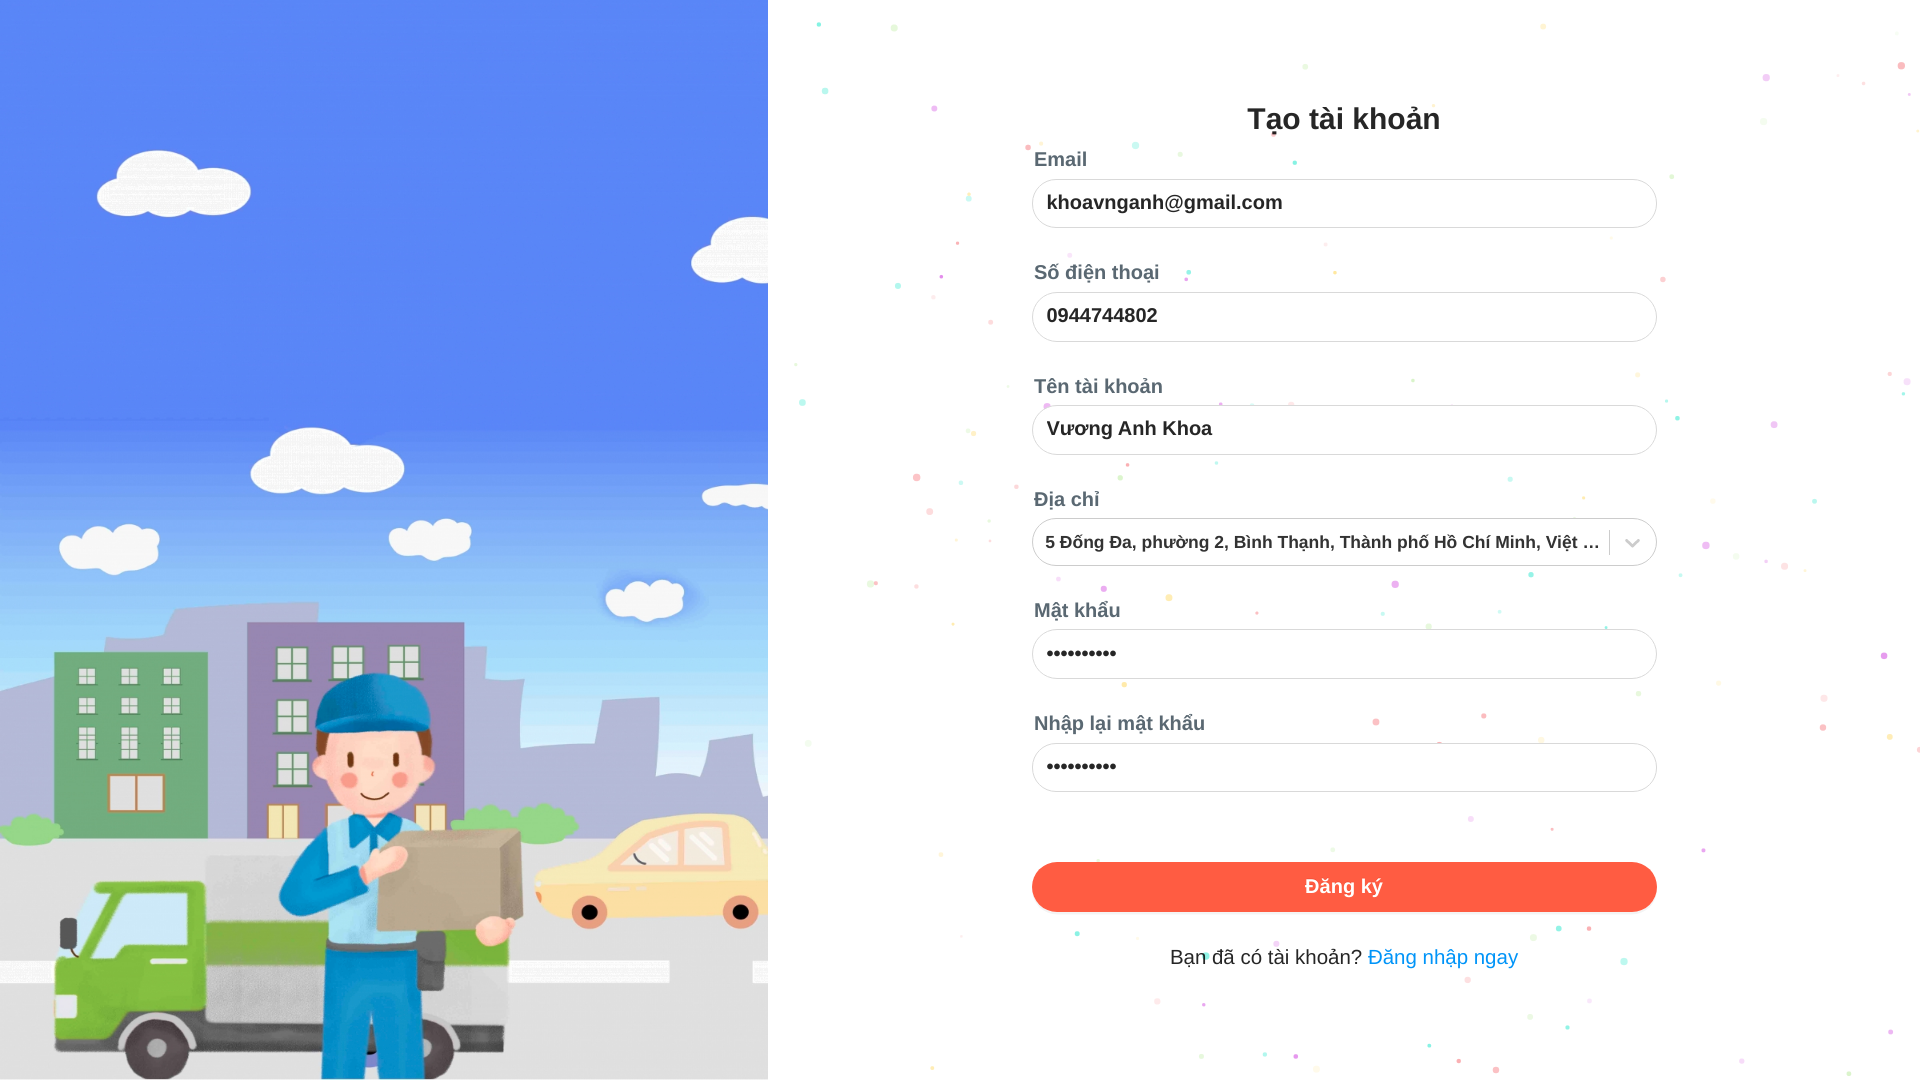
\includegraphics[width=1\textwidth]{/Auth/SignUp.png}
				\centering
				\caption{Giao diện đăng kí dành cho người muốn gửi đơn hàng}
			\end{figure}
		
		\item \textbf{Đăng nhập}
		\begin{figure}[H]
			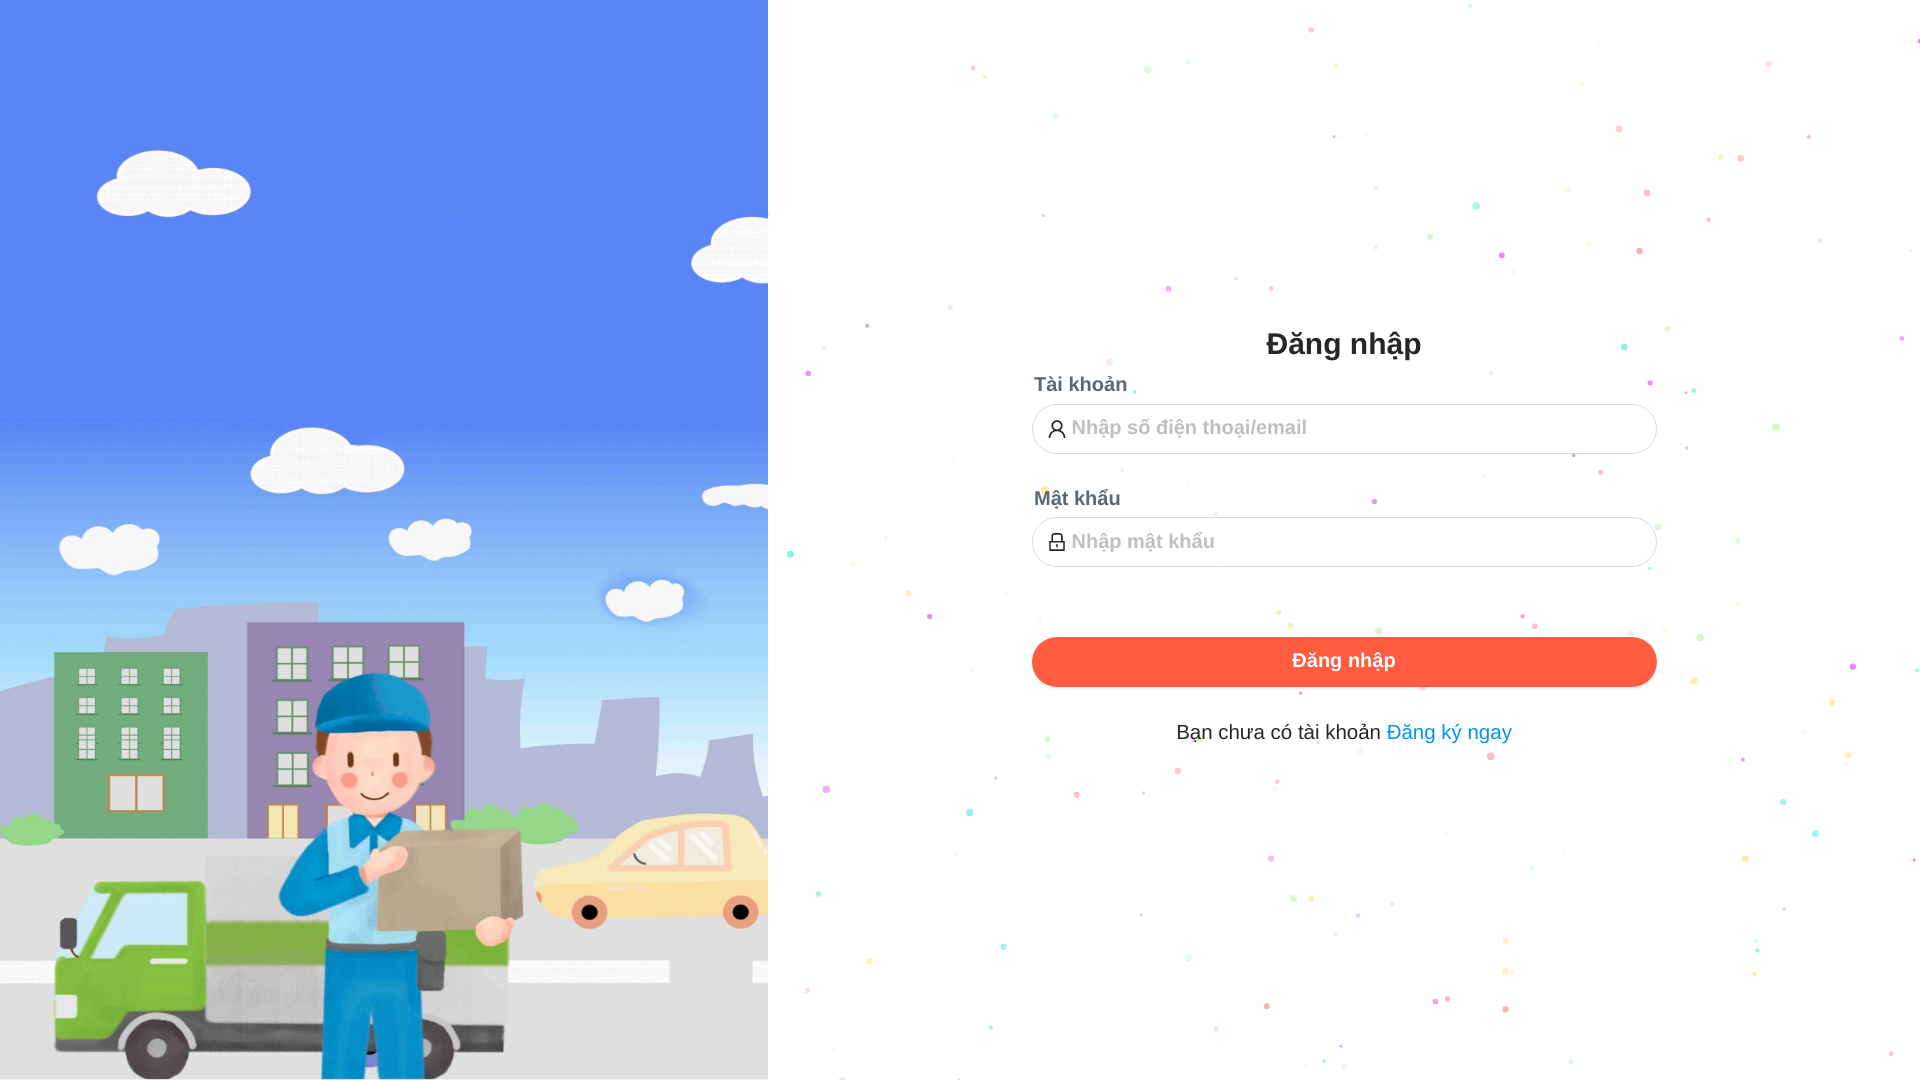
\includegraphics[width=1\textwidth]{/Auth/SignIn.png}
			\centering
			\caption{Giao diện đăng nhập dành cho actor của hệ thống}
		\end{figure}
	\end{itemize}

\subsection{Chức năng dành cho người gửi}
	\begin{itemize}
		\item \textbf{Lên đơn hàng}
		\begin{figure}[H]
			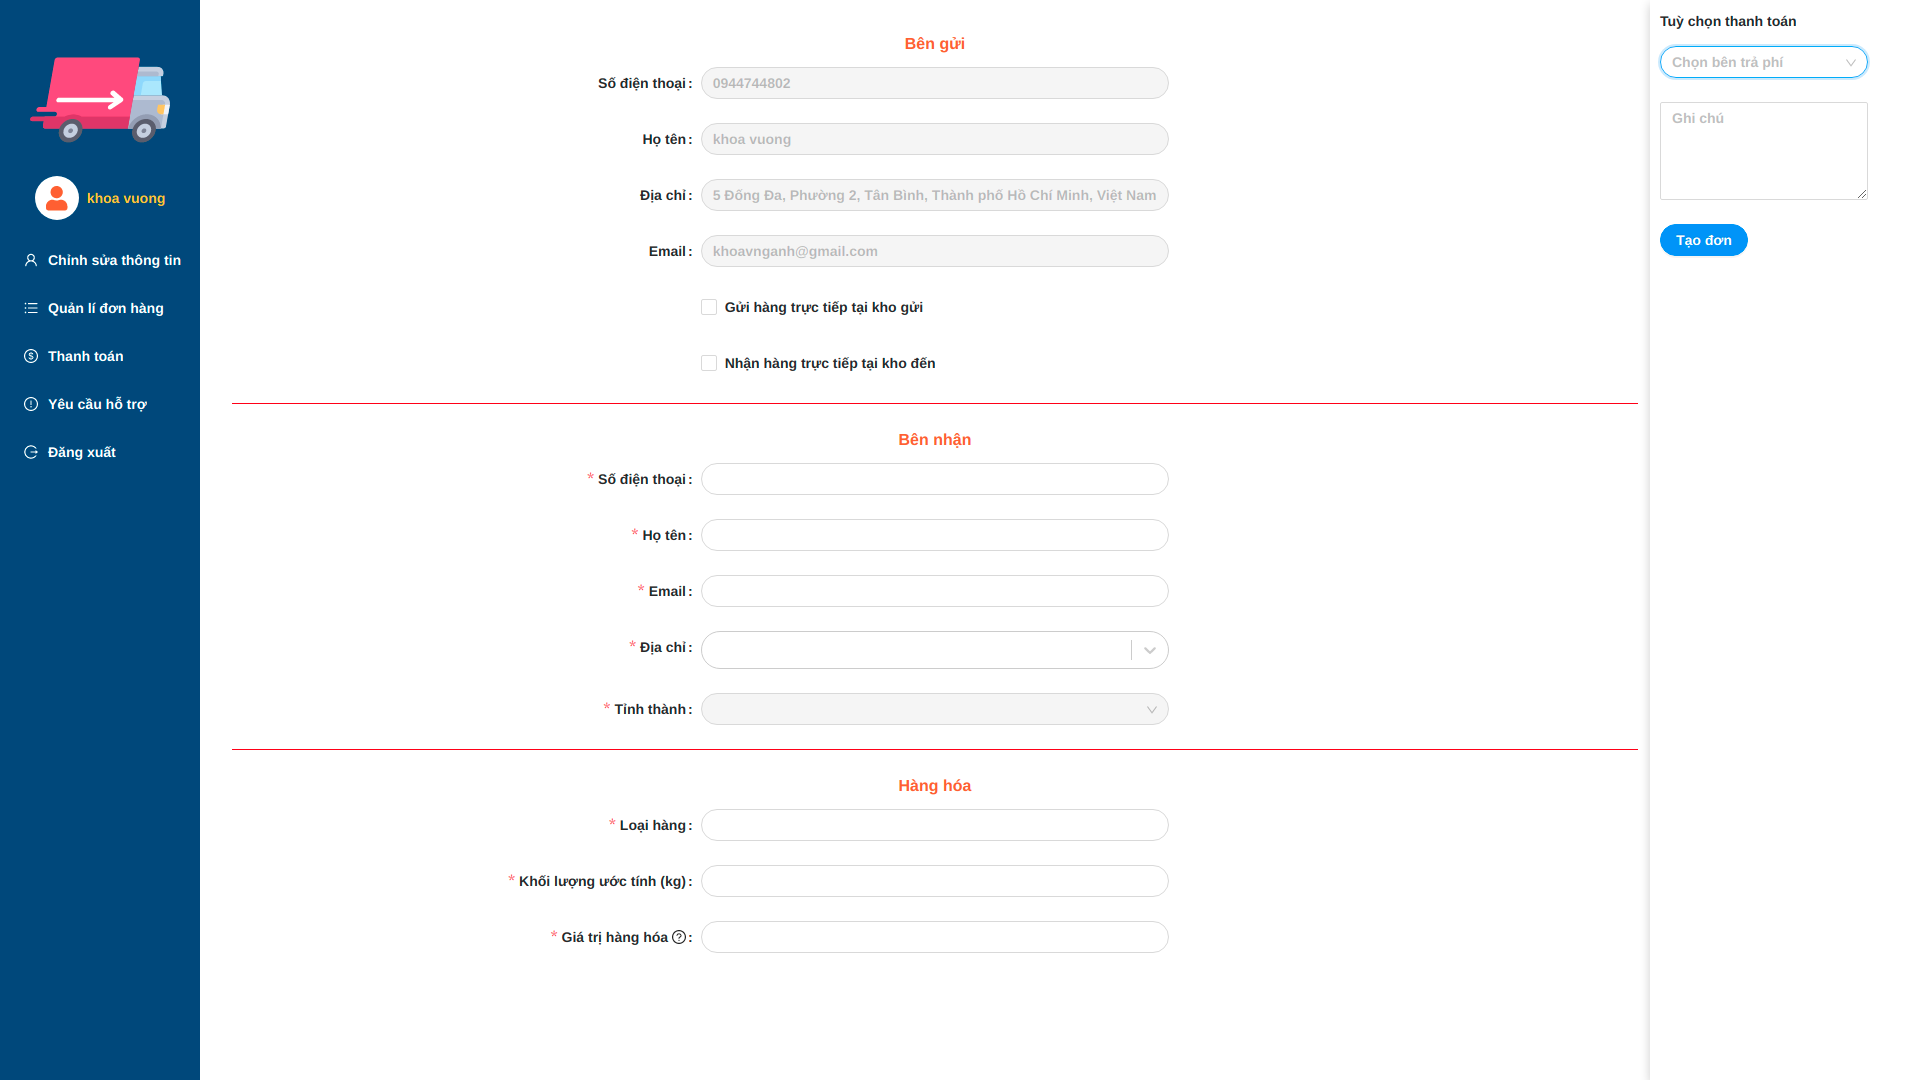
\includegraphics[width=1\textwidth]{/sender/create_order.png}
			\centering
			\caption{Giao diện điền thông tin để lên đơn hàng}
		\end{figure}
	
		\begin{figure}[H]
			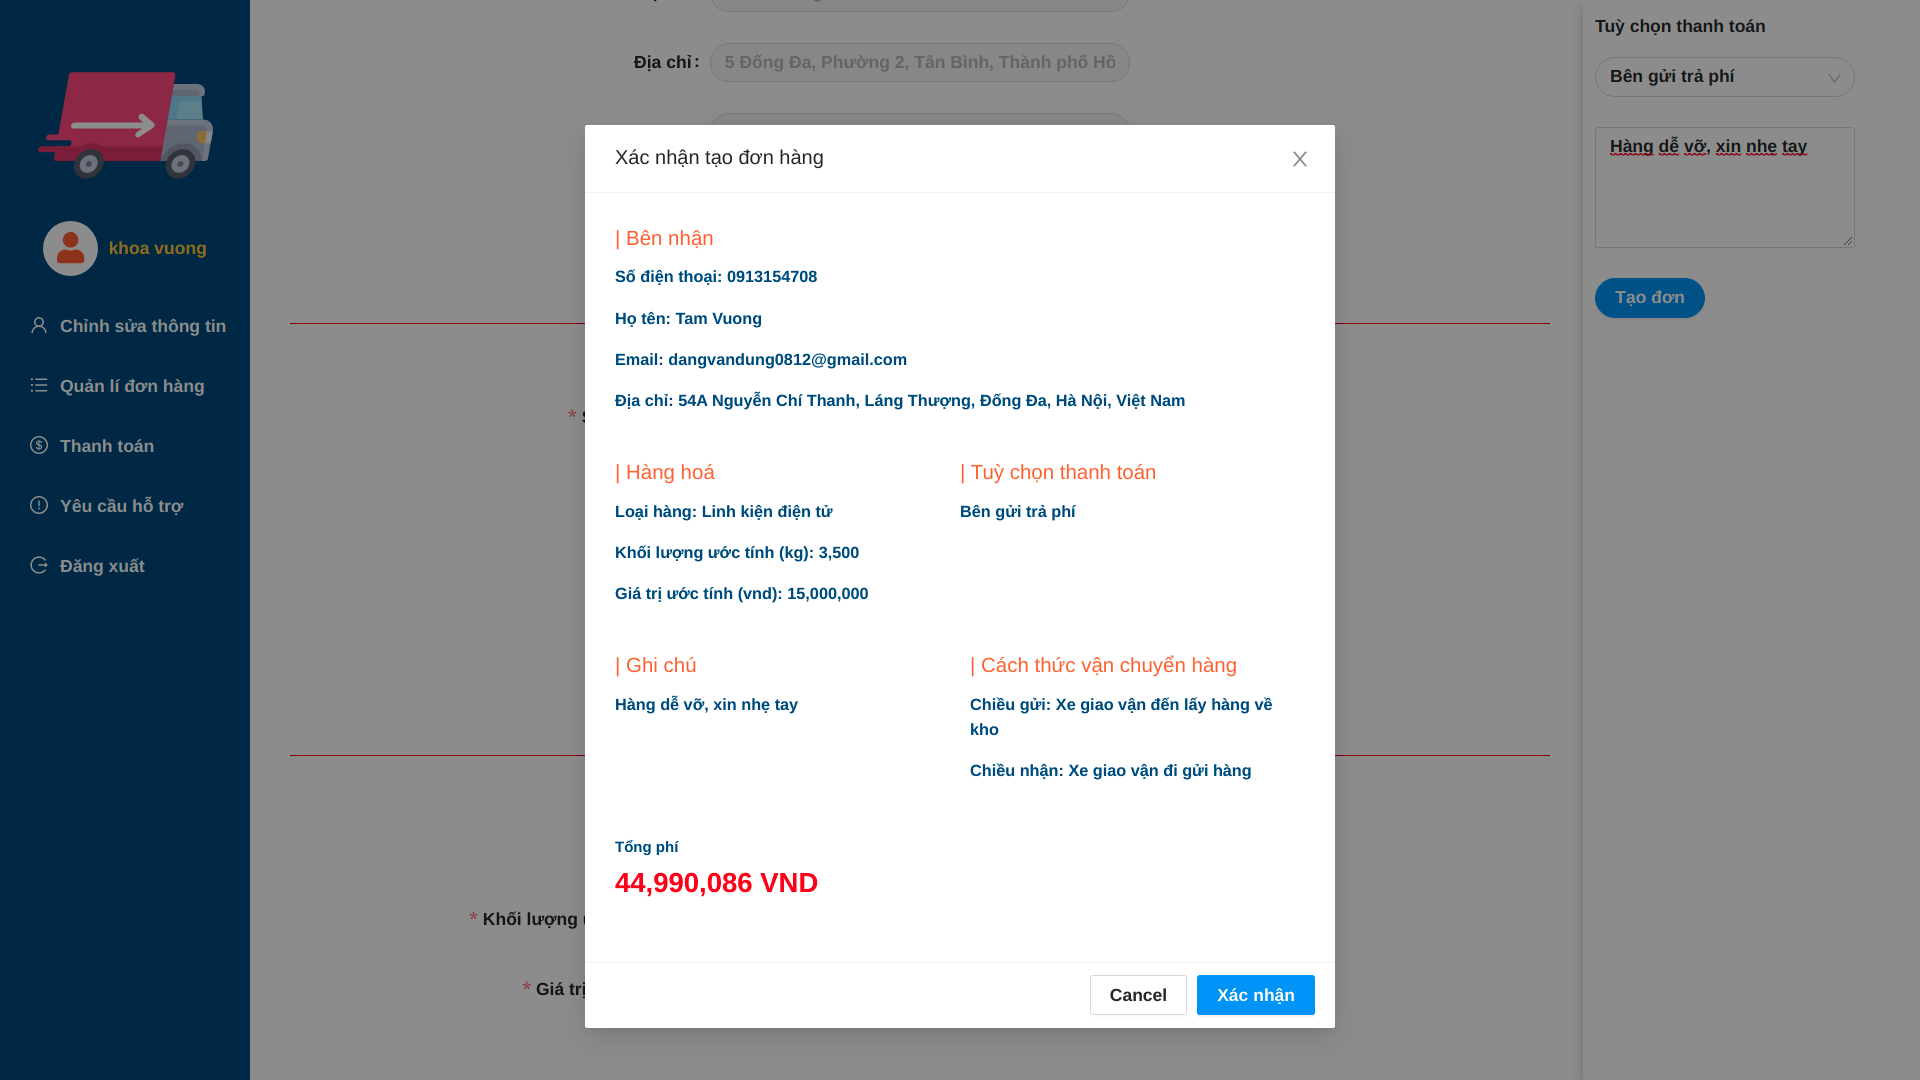
\includegraphics[width=1\textwidth]{/sender/create_order_model.png}
			\centering
			\caption{Thông tin xác nhận đơn hàng muốn tạo}
		\end{figure}
		Khung nhập địa chỉ hỗ trợ gợi ý địa chỉ nhờ sử dụng Google Place Autocomplete API. Khi ấn nút tạo đơn sẽ có màn hình chờ để phía server trả về phí vận chuyển.
		
		\item \textbf{Xem danh sách đơn hàng}
		\begin{figure}[H]
			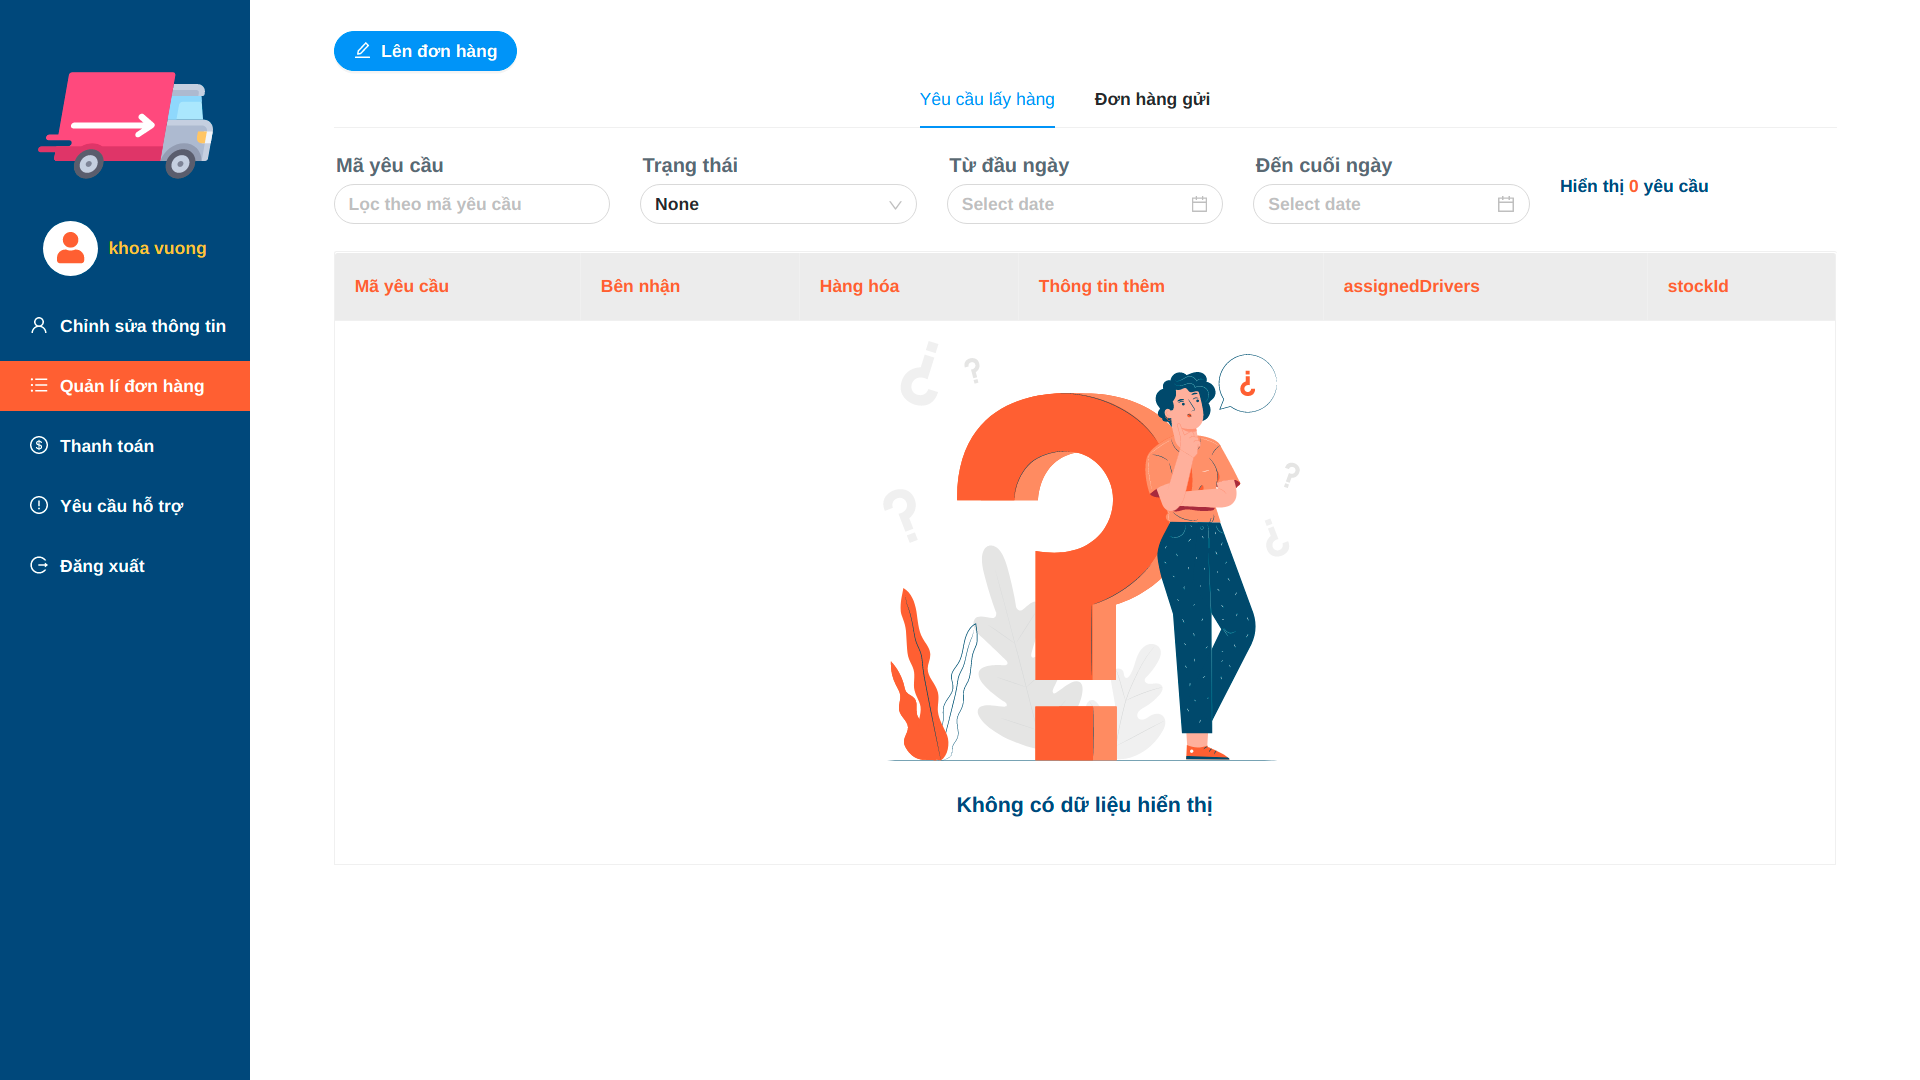
\includegraphics[width=1\textwidth]{/sender/request_empty.png}
			\centering
			\caption{Giao diện list yêu cầu của người gửi (Rỗng)}
		\end{figure}
		
		\begin{figure}[H]
			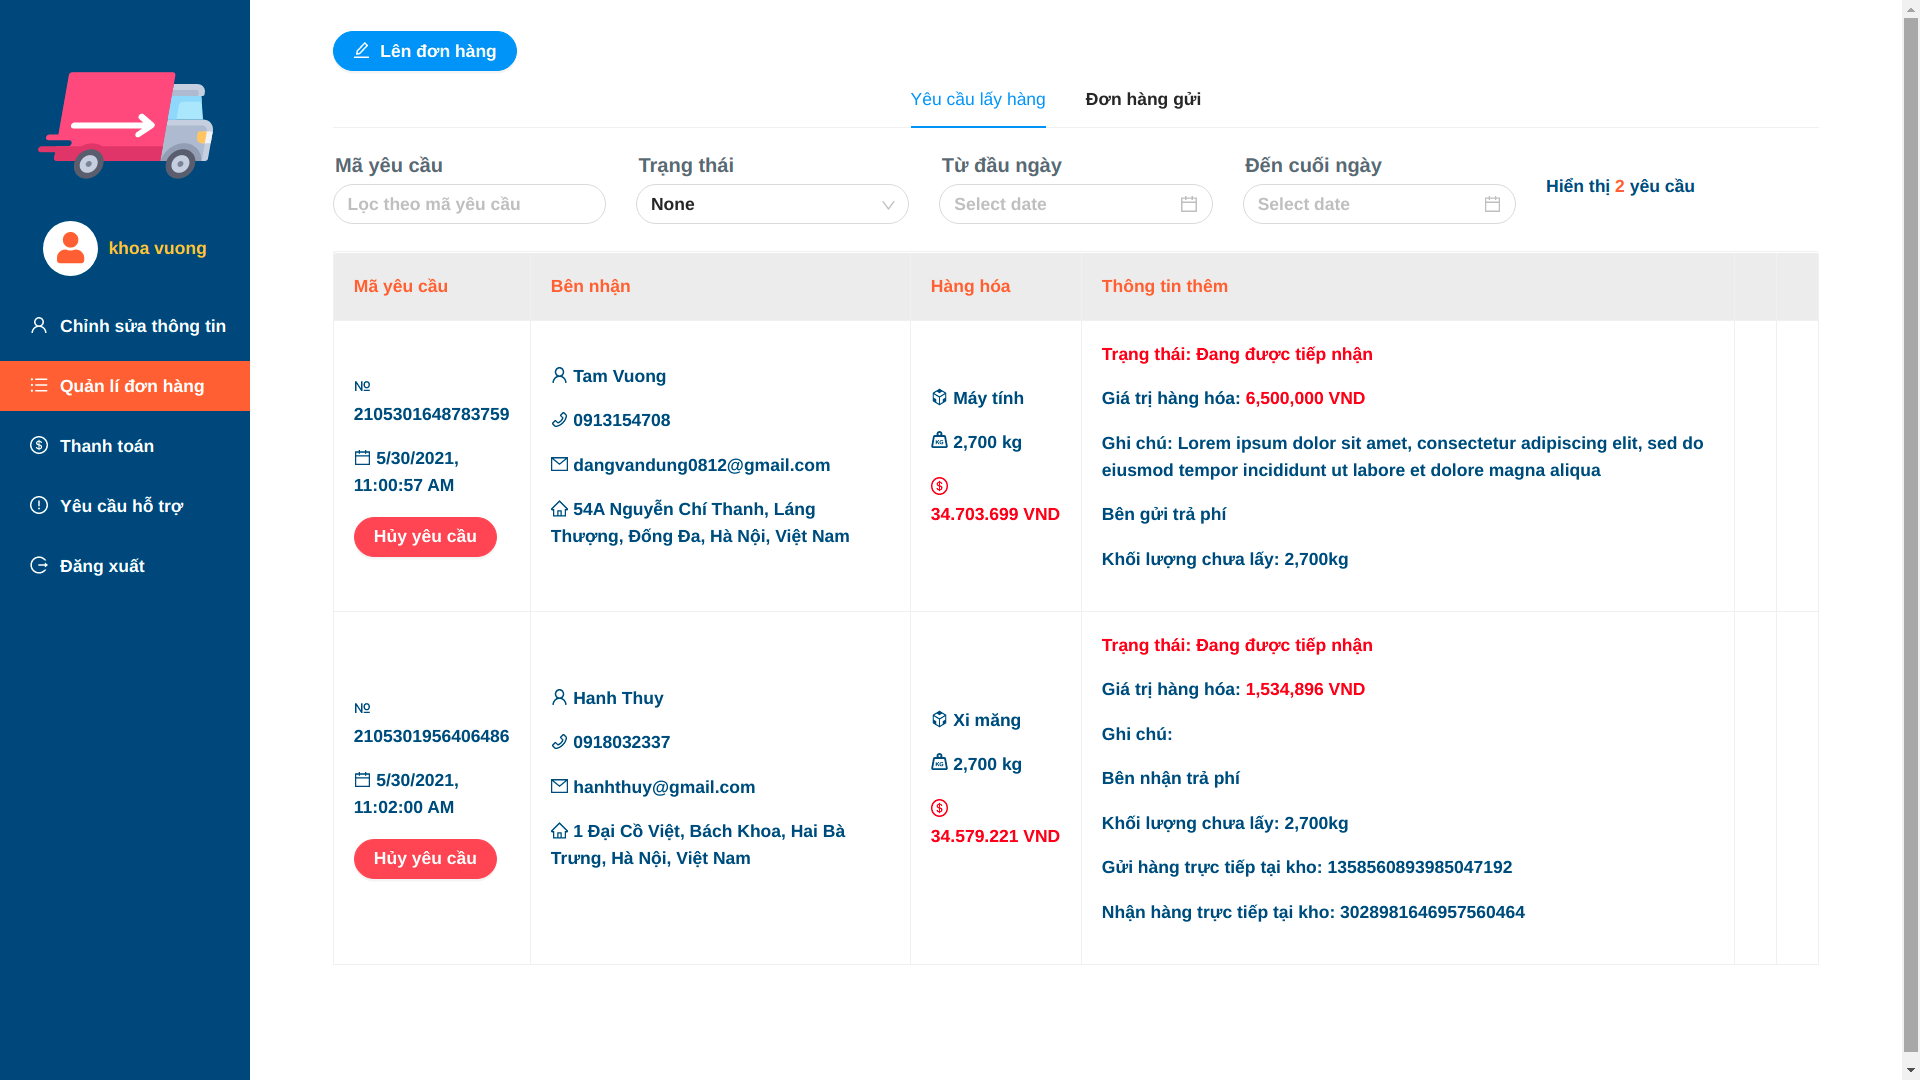
\includegraphics[width=1\textwidth]{/sender/request_list.png}
			\centering
			\caption{Giao diện list yêu cầu của người gửi (Có yêu cầu)}
		\end{figure}
		Các yêu cầu đã tạo có thể được lọc theo những tiêu chí: Mã yêu cầu, trạng thái (Gồm 4 trạng thái yêu cầu đã nêu trong phần trước), thời gian tạo đơn hàng.
		
		\item \textbf{Xem danh sách các kiện hàng}
		\begin{figure}[H]
			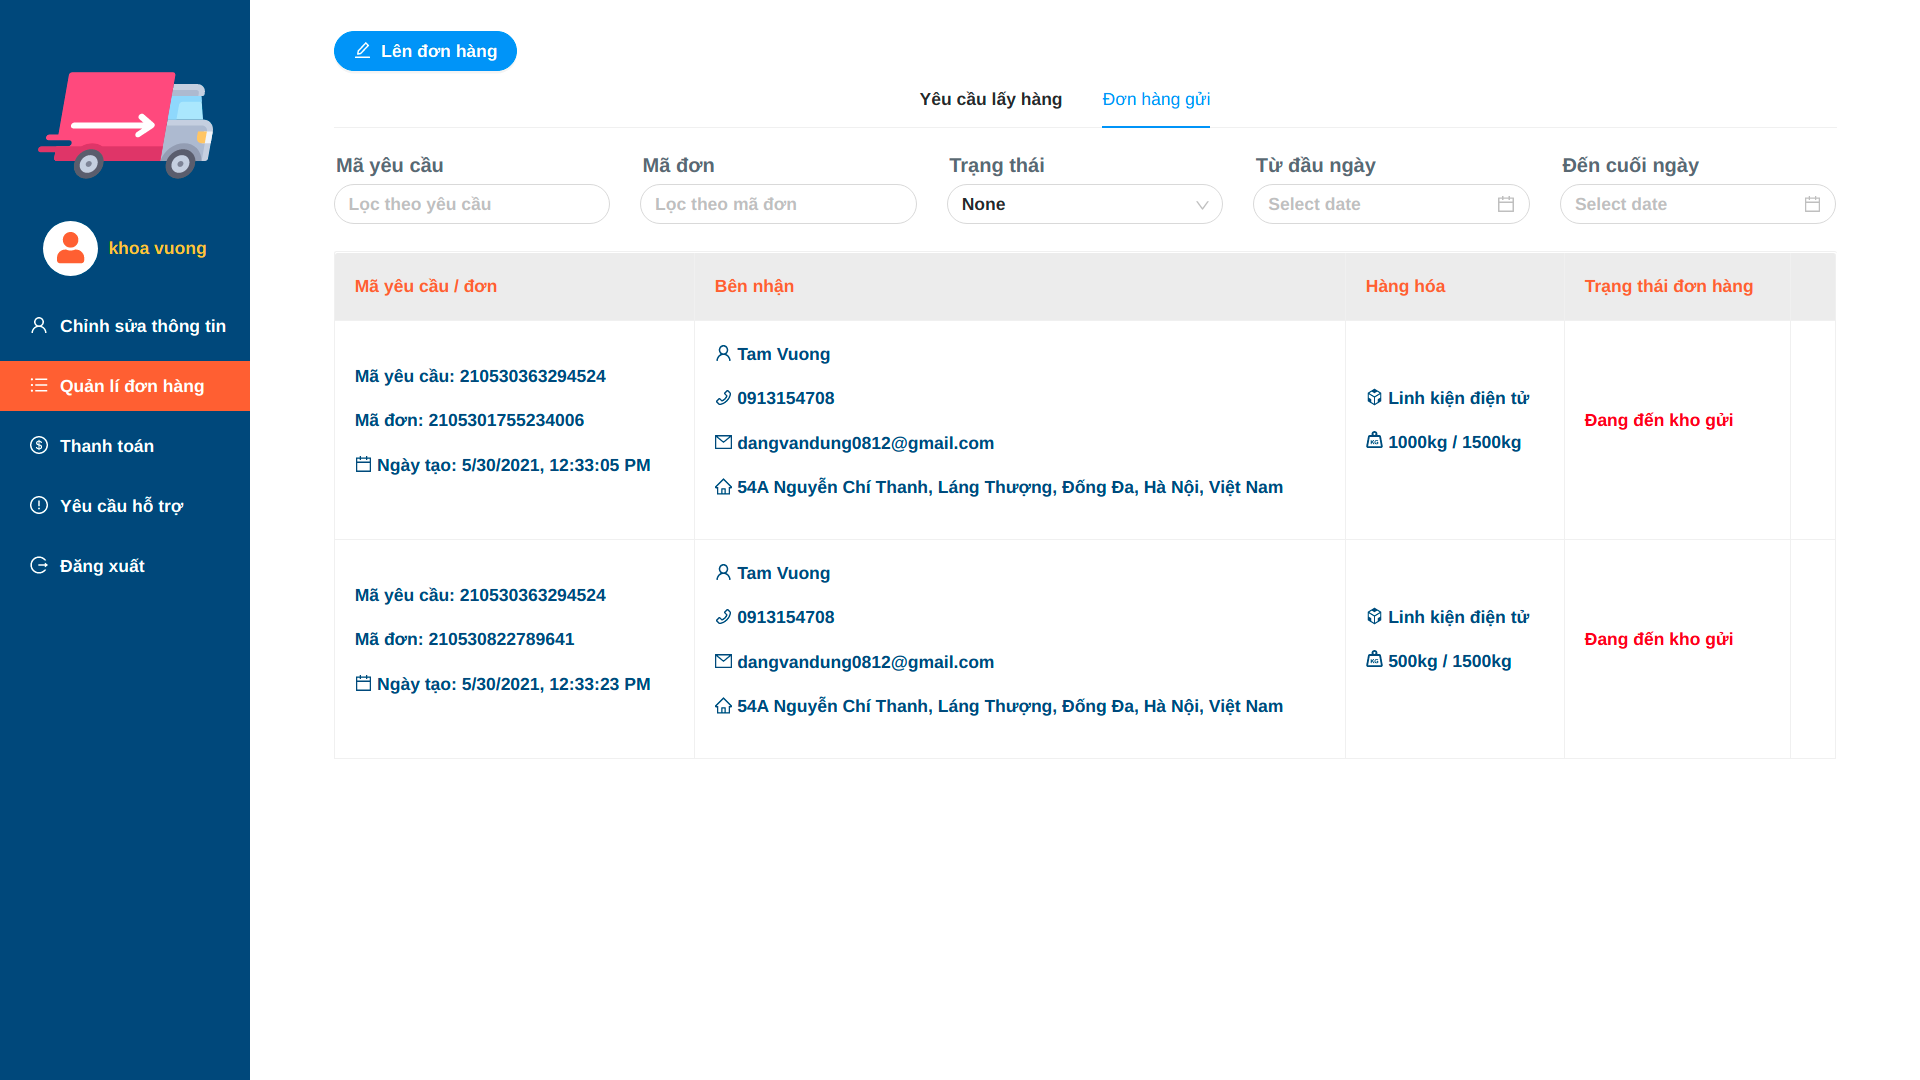
\includegraphics[width=1\textwidth]{/sender/sender_suborders.png}
			\centering
			\caption{Giao diện xem danh sách các đơn hàng nhỏ được tách từ yêu cầu}
		\end{figure}
	
		\item \textbf{Chỉnh sửa thông tin của người gửi}
		
		\begin{figure}[H]
			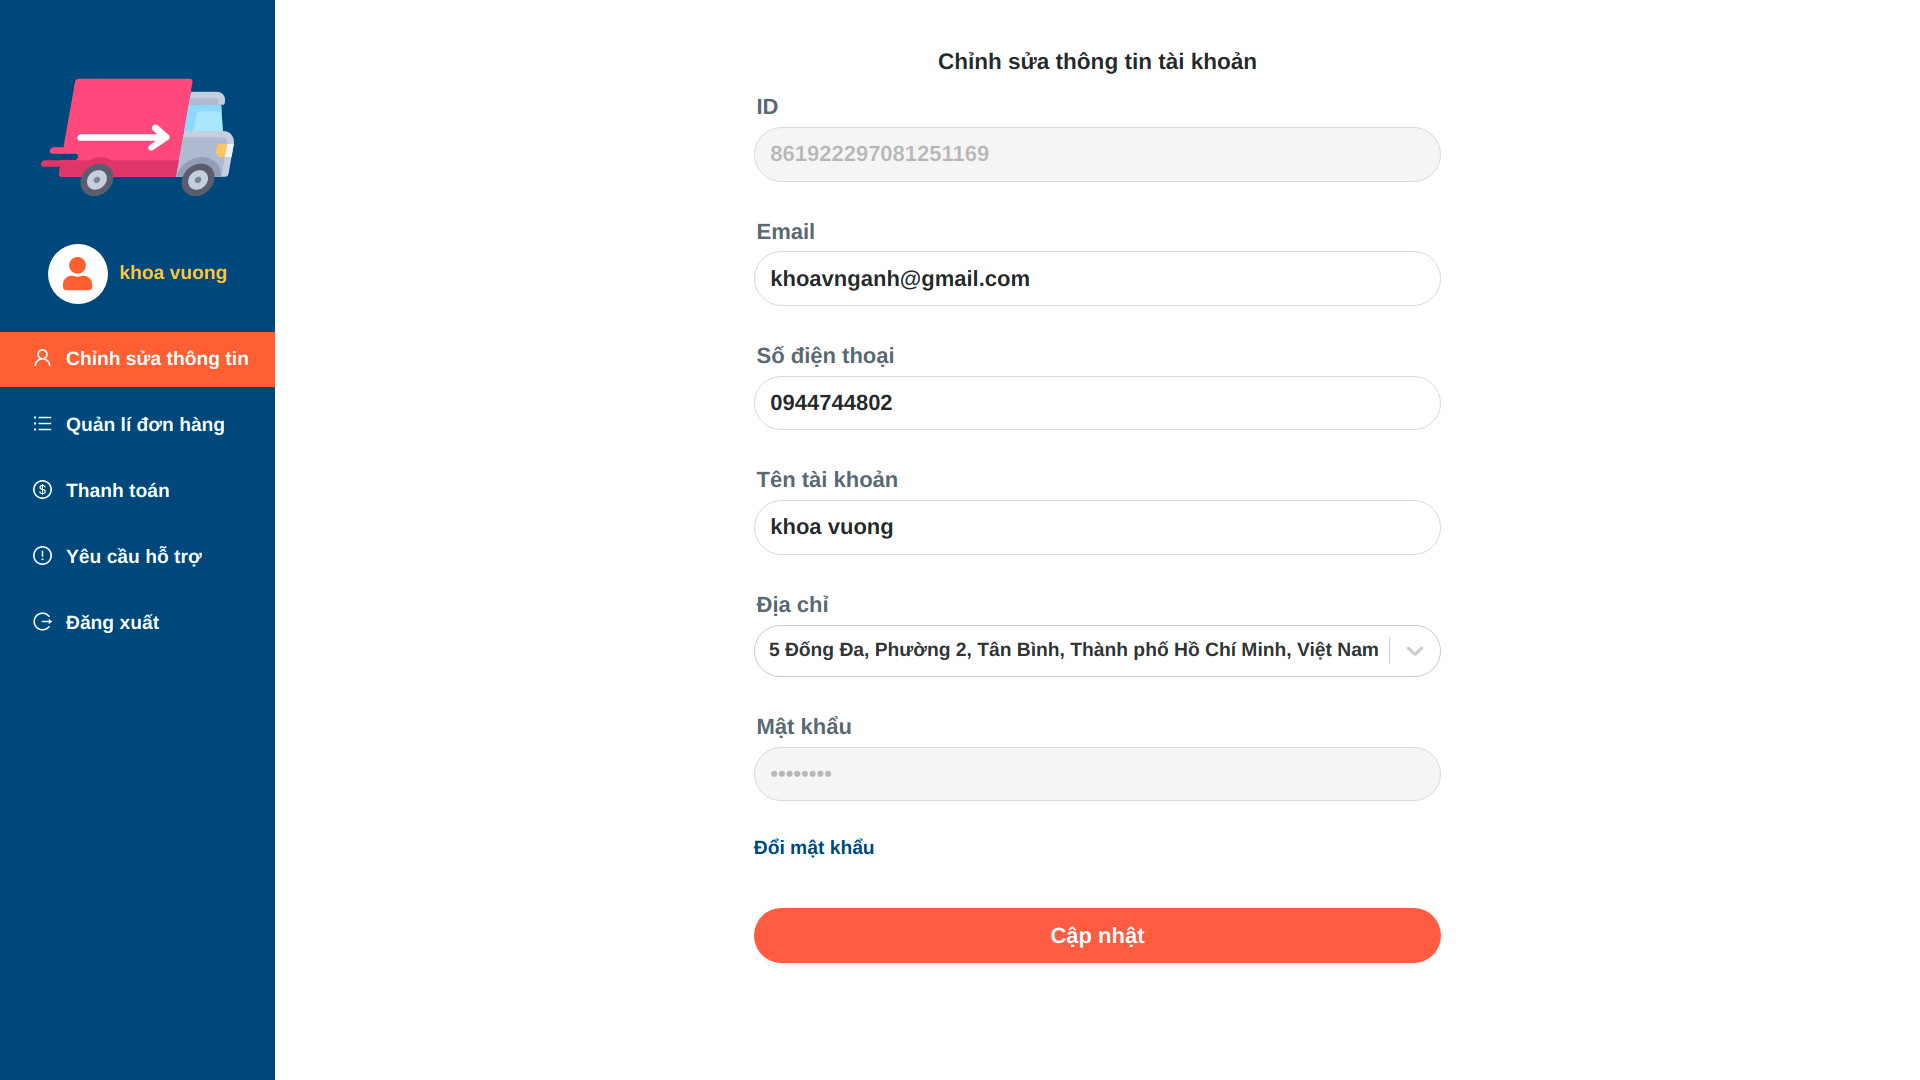
\includegraphics[width=1\textwidth]{/sender/sender_info.png}
			\centering
			\caption{Giao diện chỉnh sửa thông tin của người gửi}
		\end{figure}
		
		
	\end{itemize}


\subsection{Chức năng dành cho tài xế}
\begin{itemize}
	\item \textbf{Tìm những yêu cầu được gán}
	\begin{figure}[H]
		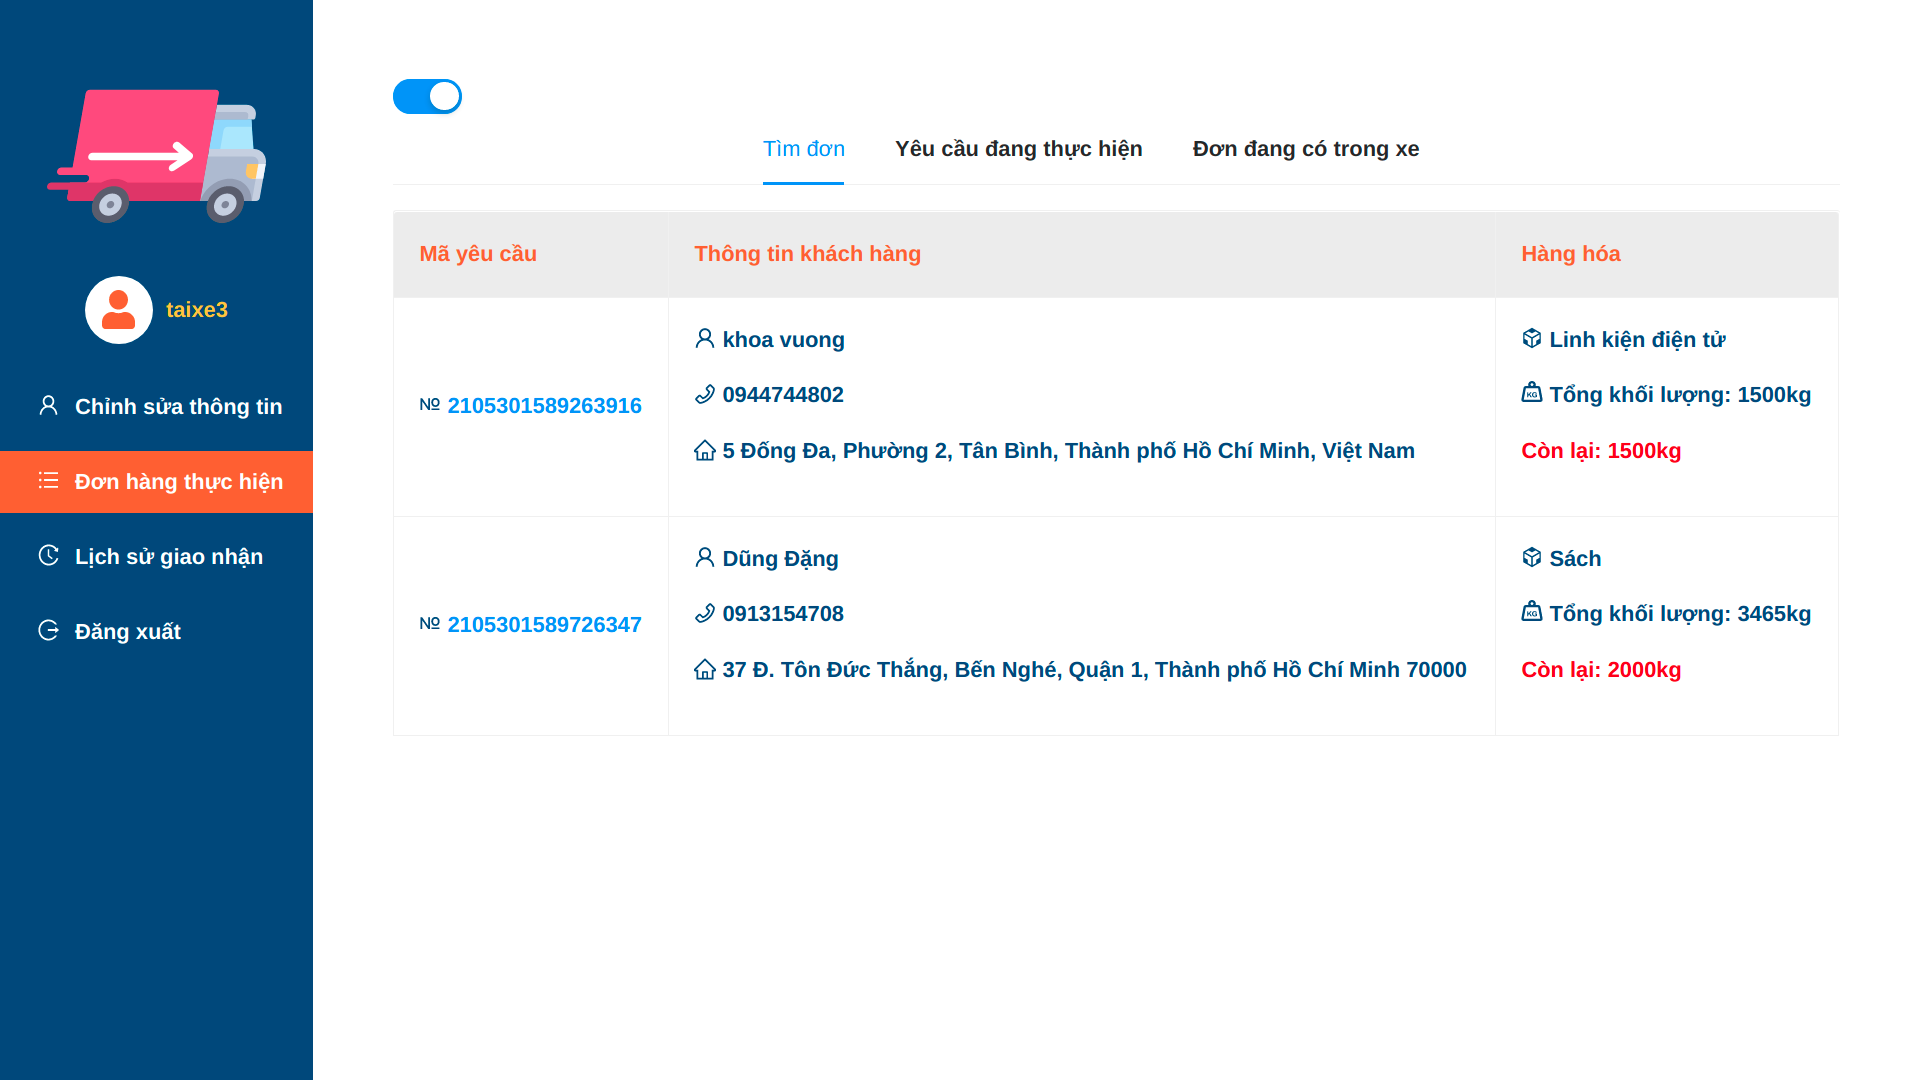
\includegraphics[width=1\textwidth]{/driver/driver_find_order.png}
		\centering
		\caption{Giao diện tìm những yêu cầu được gán}
	\end{figure}
	
	\begin{figure}[H]
		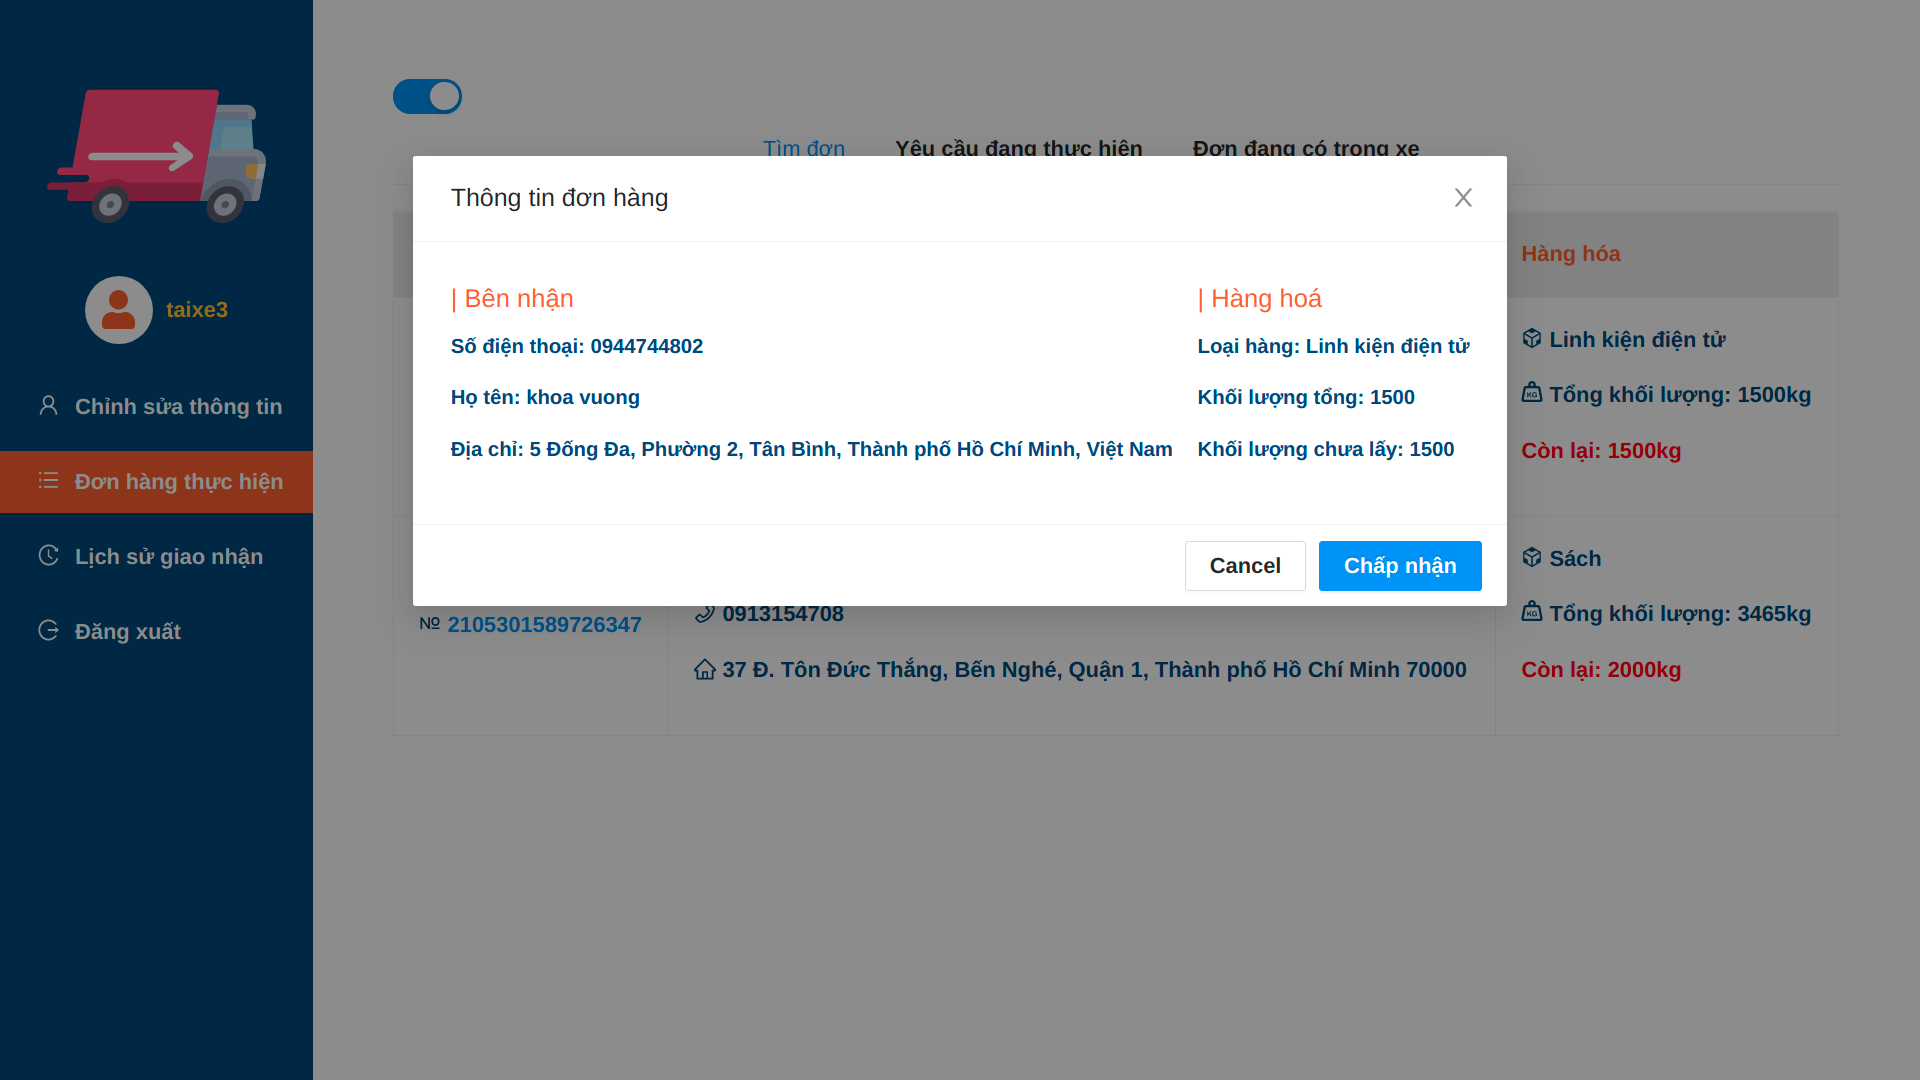
\includegraphics[width=1\textwidth]{/driver/driver_find_modal.png}
		\centering
		\caption{Giao diện xác nhận lại thông tin yêu cầu muốn nhận}
	\end{figure}
	
	
	\item \textbf{Xem danh sách đơn hàng}
	\begin{figure}[H]
		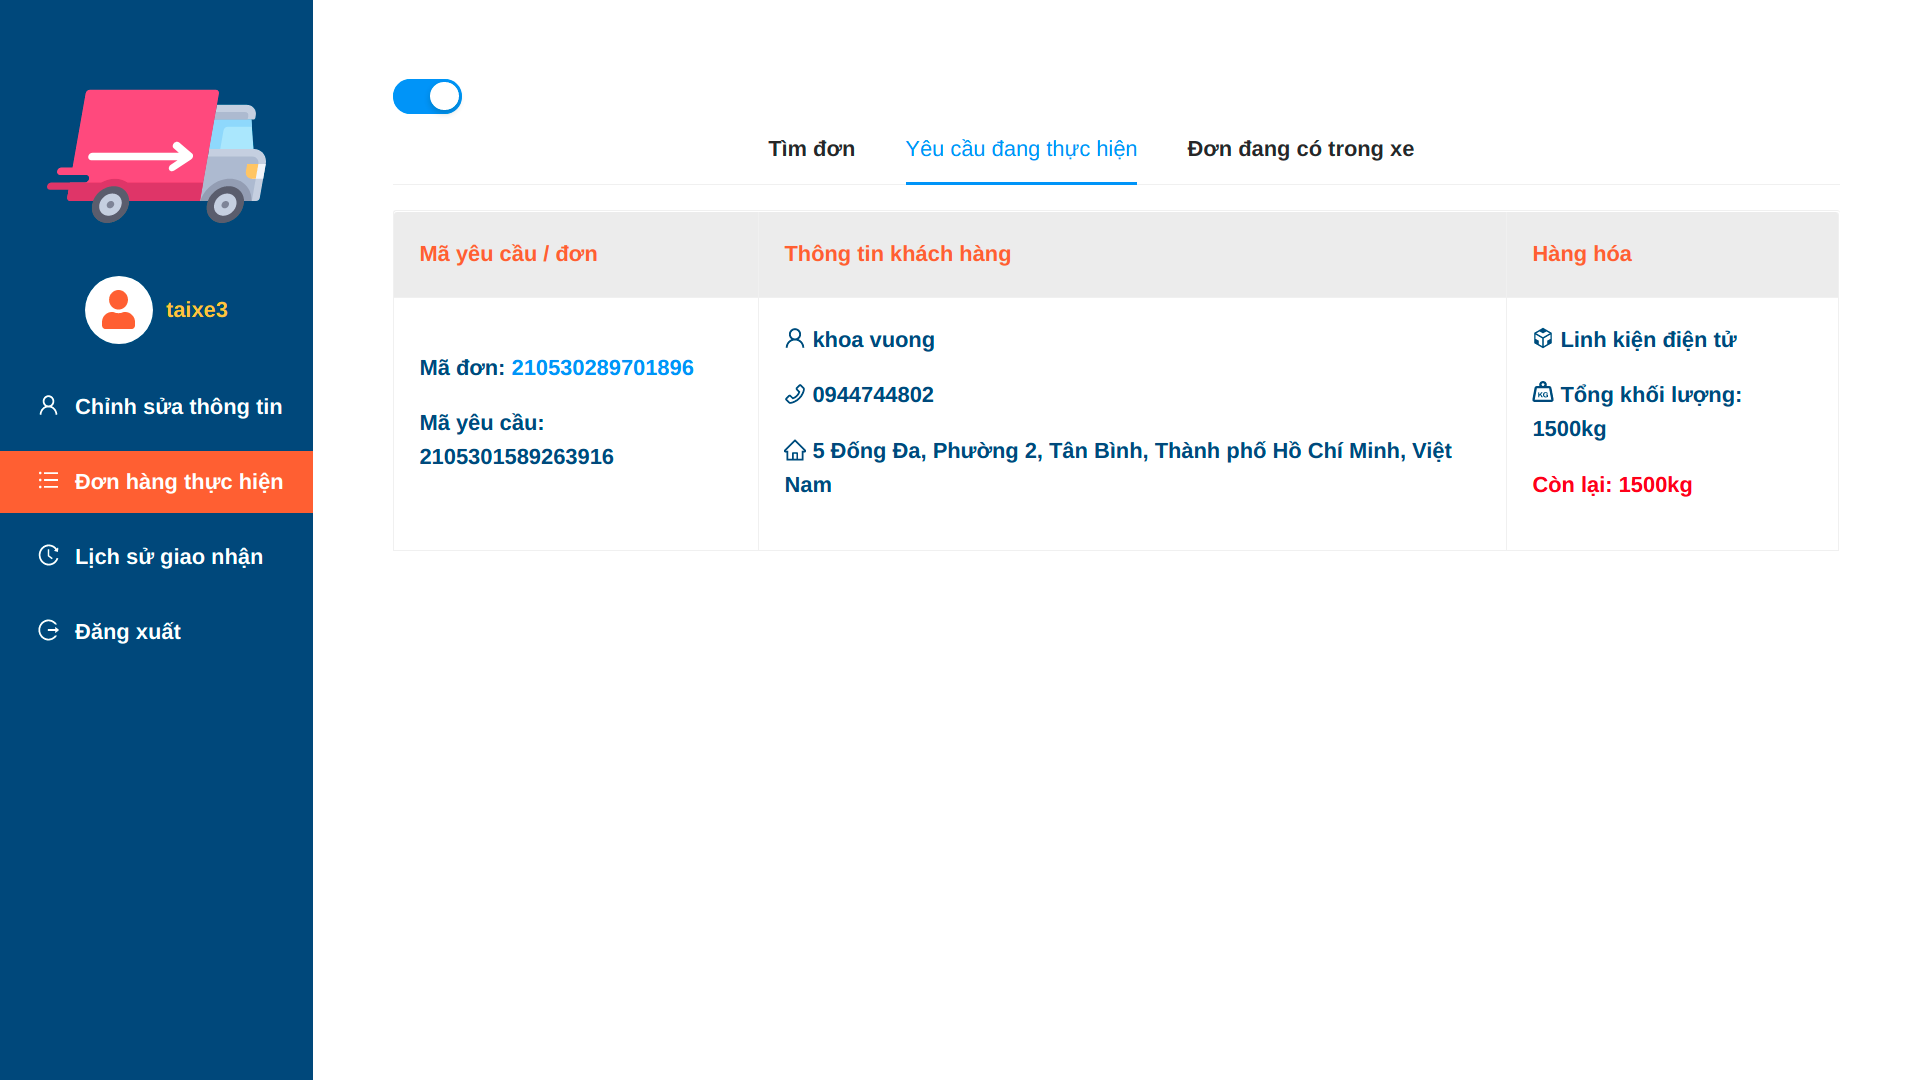
\includegraphics[width=1\textwidth]{/driver/driver_current_order.png}
		\centering
		\caption{Giao diện xem thông tin đơn hàng đang đến lấy}
	\end{figure}
	
	\begin{figure}[H]
		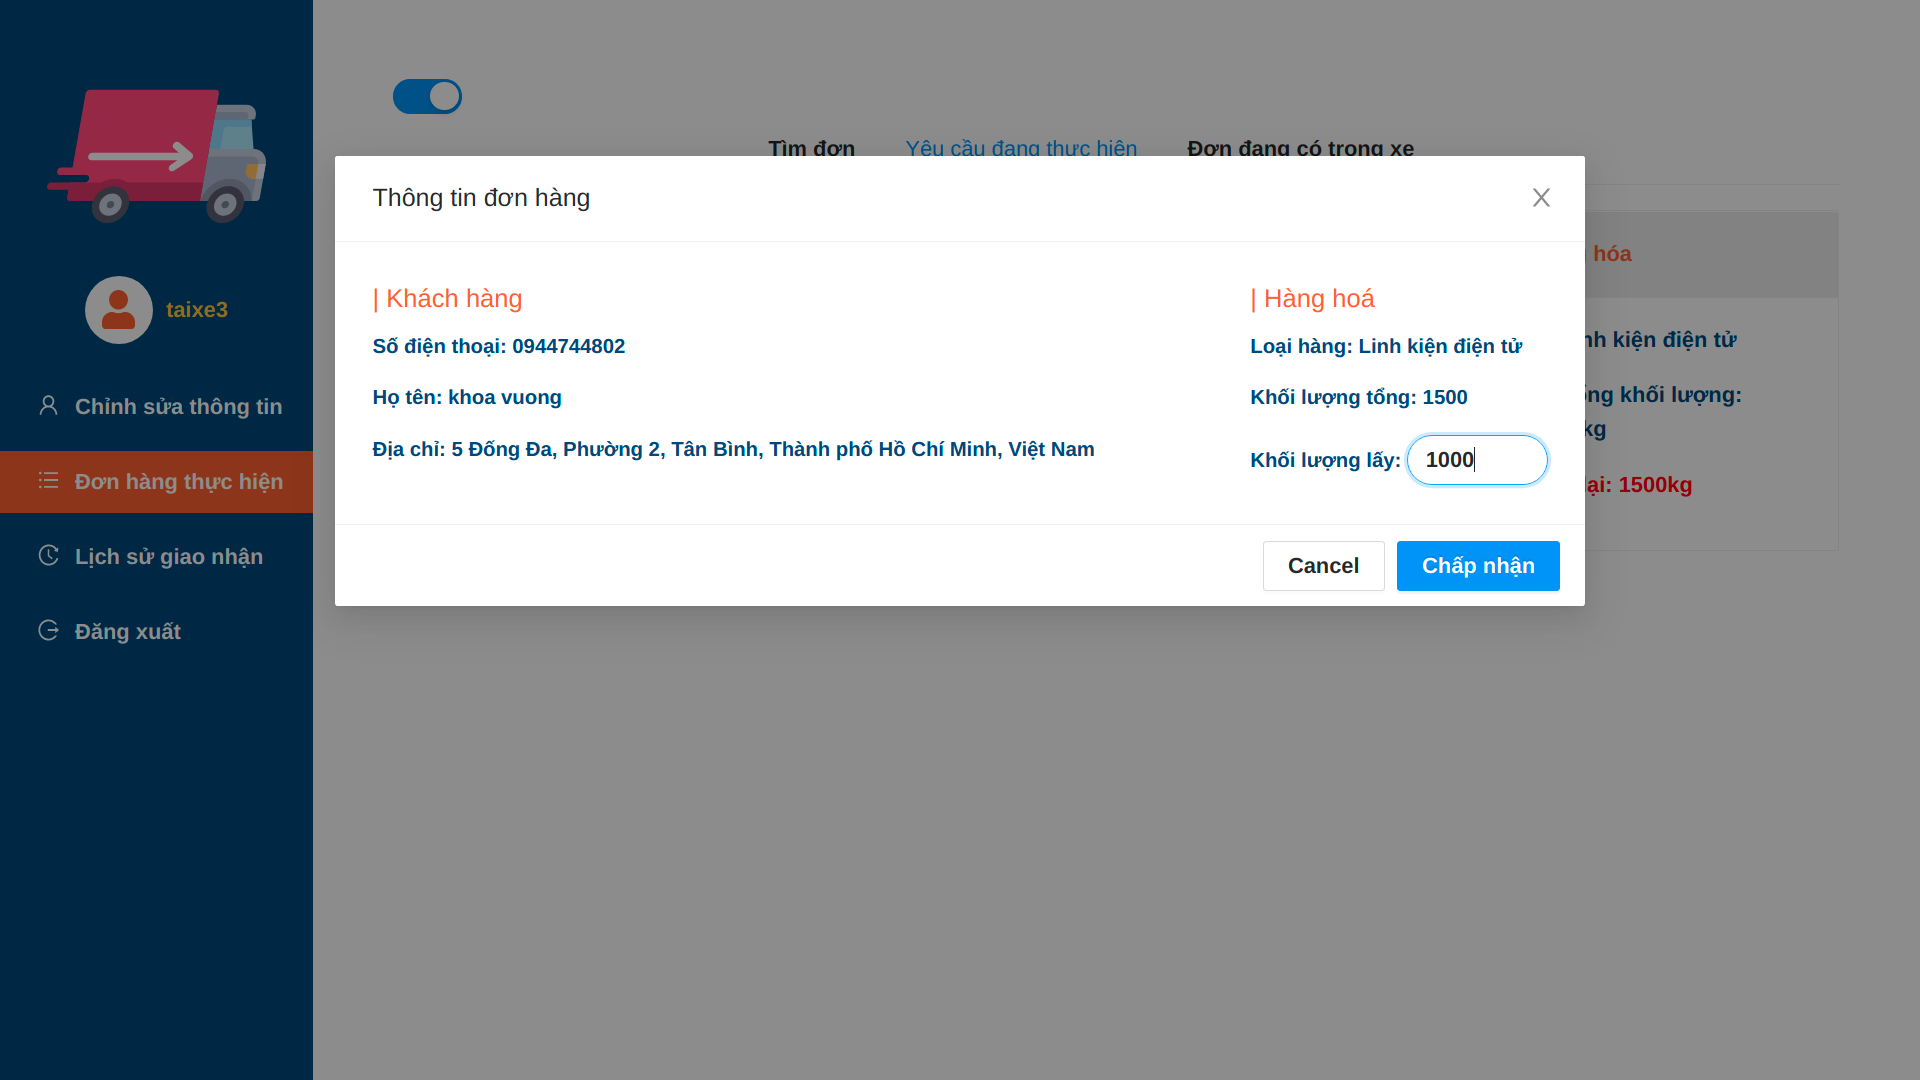
\includegraphics[width=1\textwidth]{/driver/driver_current_modal.png}
		\centering
		\caption{Giao diện xác nhận lại thông tin đơn hàng đang muốn nhận}
	\end{figure}


	
	\item \textbf{Xem danh sách các kiện hàng}
	\begin{figure}[H]
		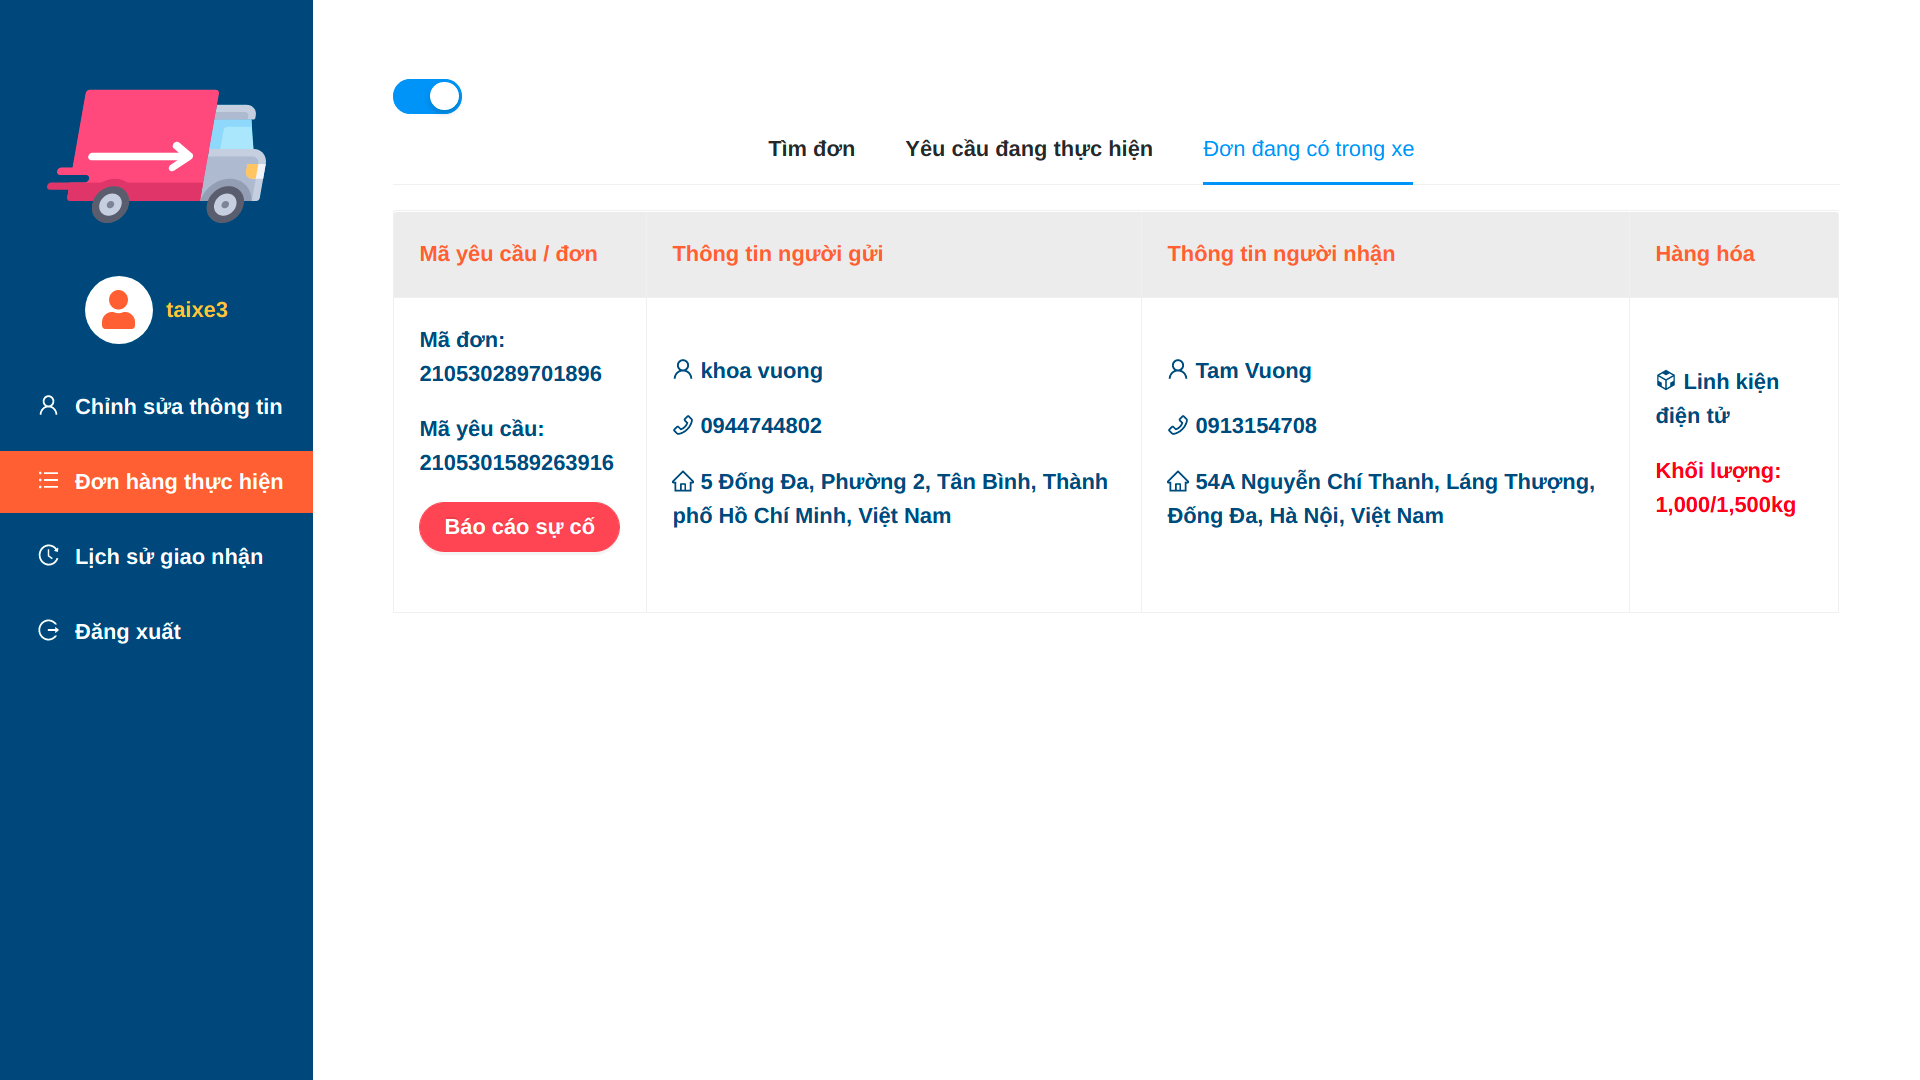
\includegraphics[width=1\textwidth]{/driver/driver_intruck.png}
		\centering
		\caption{Giao diện xem thông tin các đơn hàng đang ở trong xe}
	\end{figure}
	
	\item \textbf{Báo cáo vấn đề}
	
	\begin{figure}[H]
		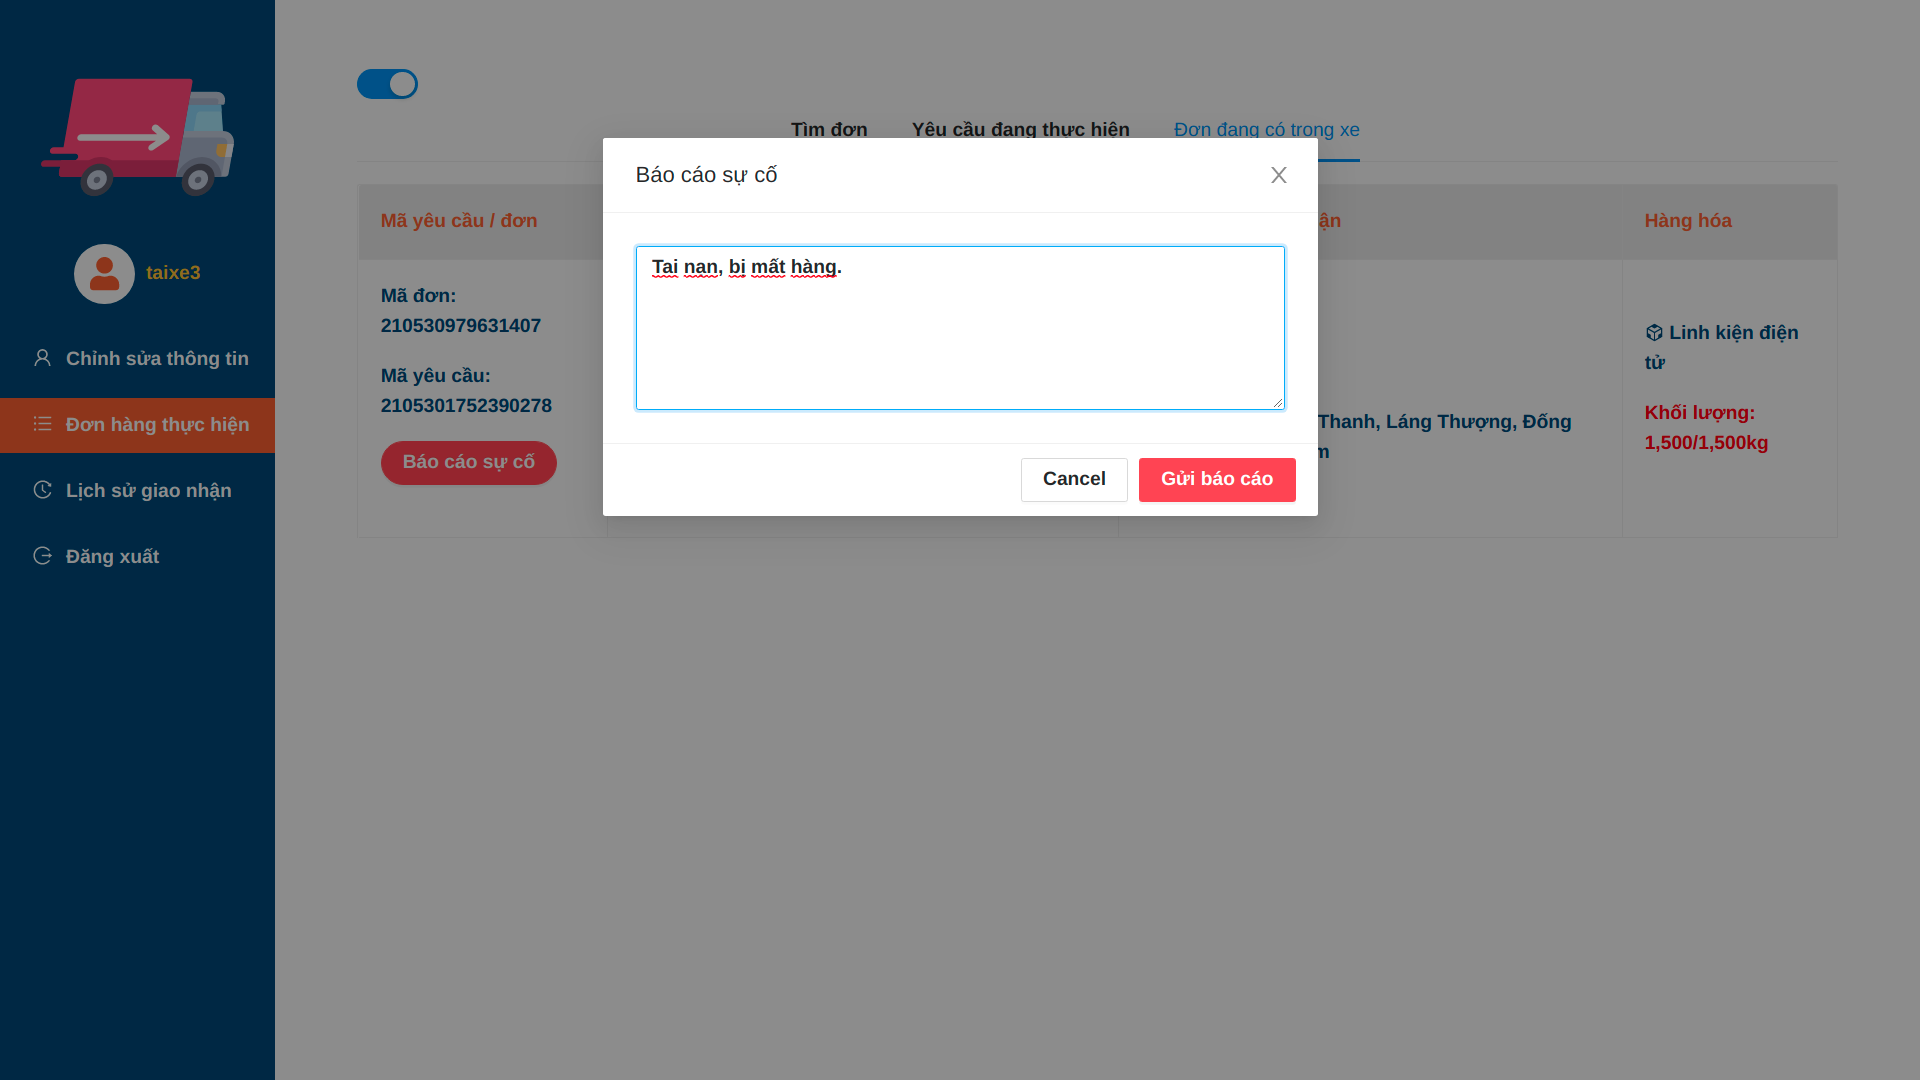
\includegraphics[width=1\textwidth]{/driver/driver_issue.png}
		\centering
		\caption{Giao diện báo cáo vấn đề ghi gặp sự cố}
	\end{figure}


	\item \textbf{Xem lịch sử giao nhận hàng}
	
	\begin{figure}[H]
		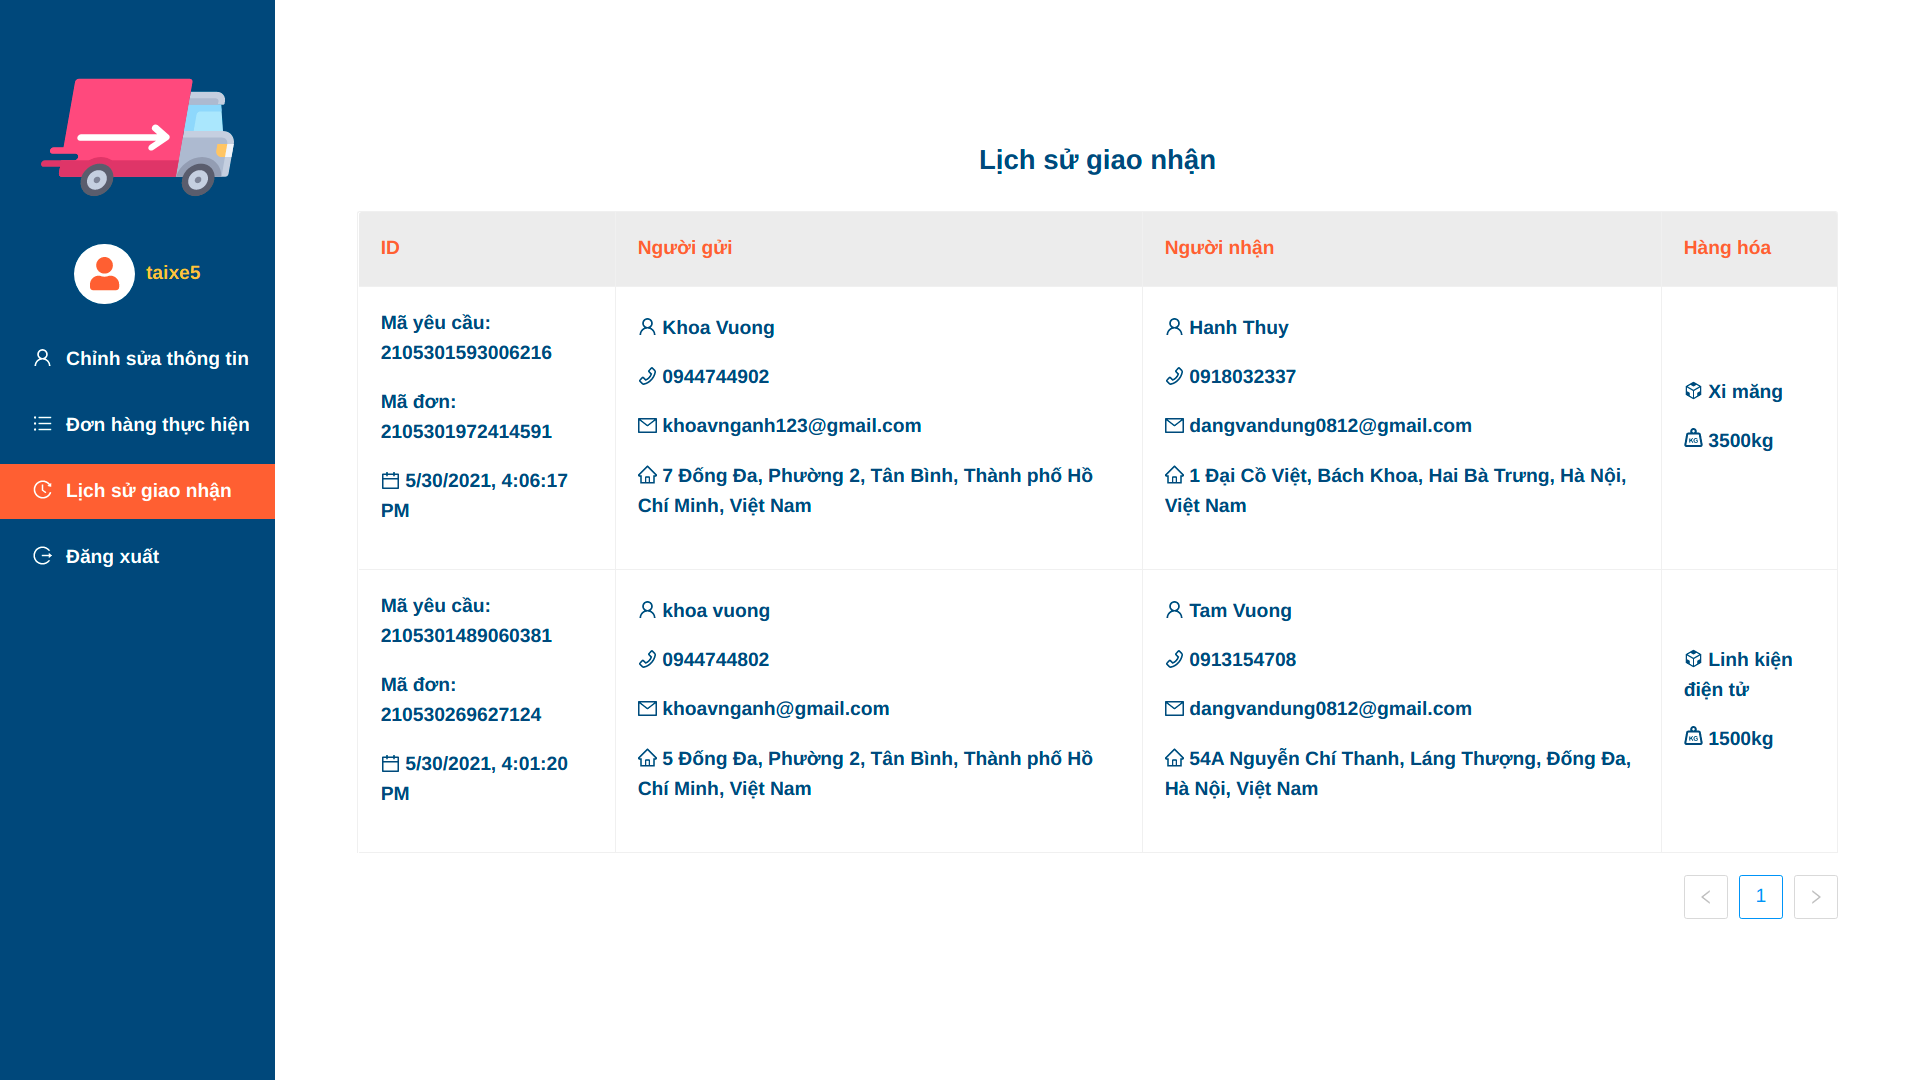
\includegraphics[width=1\textwidth]{/driver/driver_history.png}
		\centering
		\caption{Giao diện xem lịch sử giao nhận hàng}
	\end{figure}
	
\end{itemize}

\subsection{Chức năng dành cho thủ kho}
\begin{itemize}
	\item \textbf{Nhập hàng}
	\begin{figure}[H]
		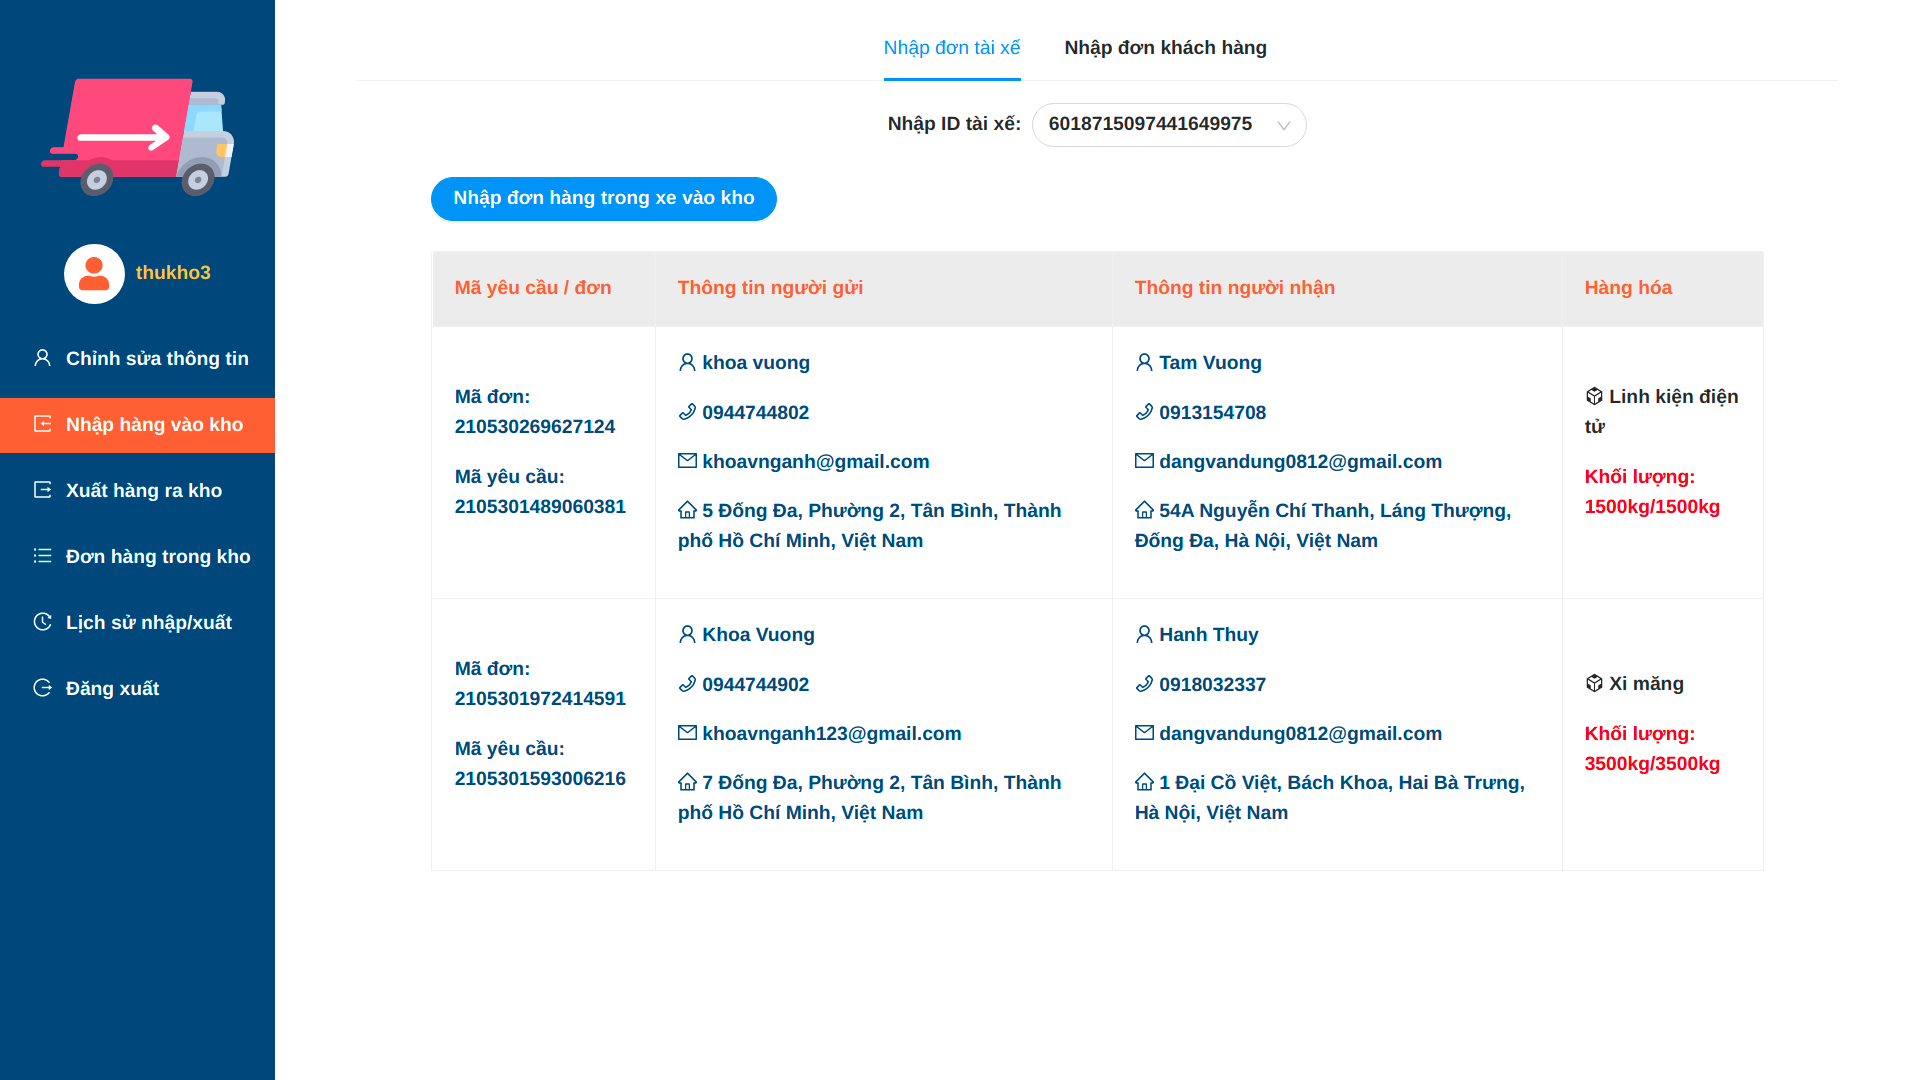
\includegraphics[width=1\textwidth]{/stockkeeper/stock_import_driver.png}
		\centering
		\caption{Giao diện nhập ID của tài xế để nhập các đơn hàng trong xe tài xế vào kho}
	\end{figure}

	\begin{figure}[H]
		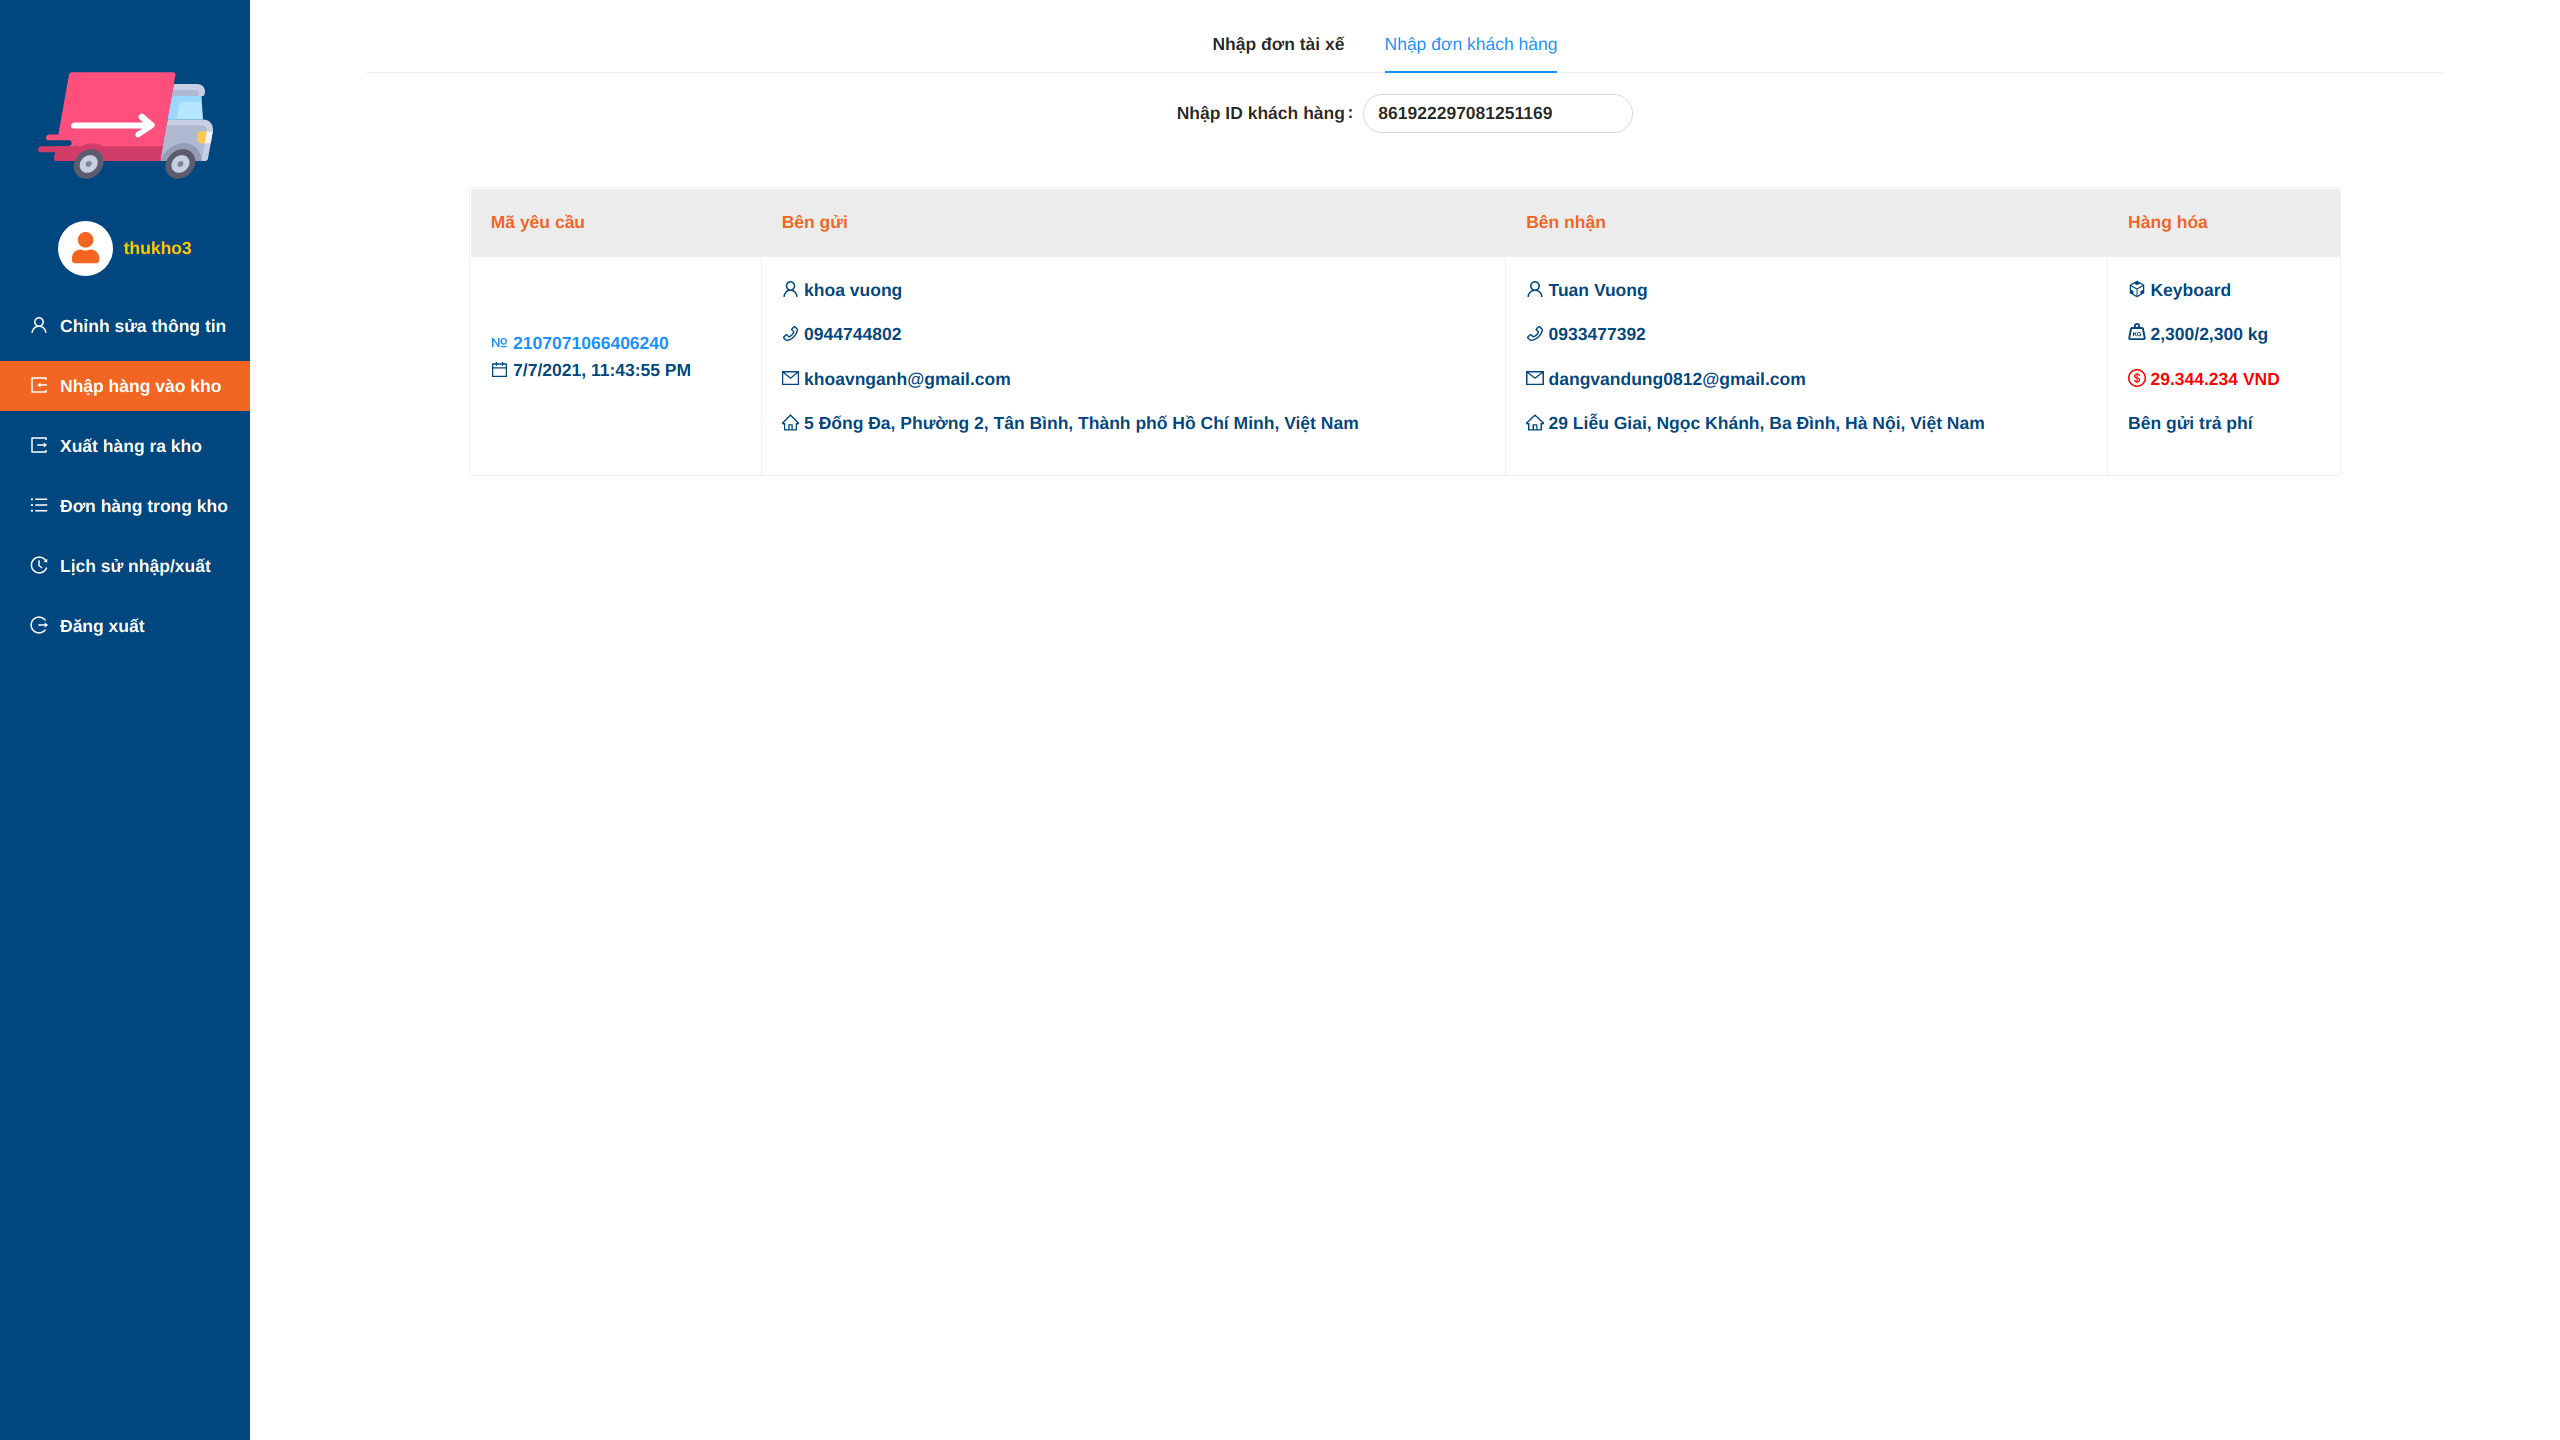
\includegraphics[width=1\textwidth]{/stockkeeper/stock_import_customer.png}
		\centering
		\caption{Nhập ID của khách hàng để nhập đơn vào kho}
	\end{figure}

	\begin{figure}[H]
		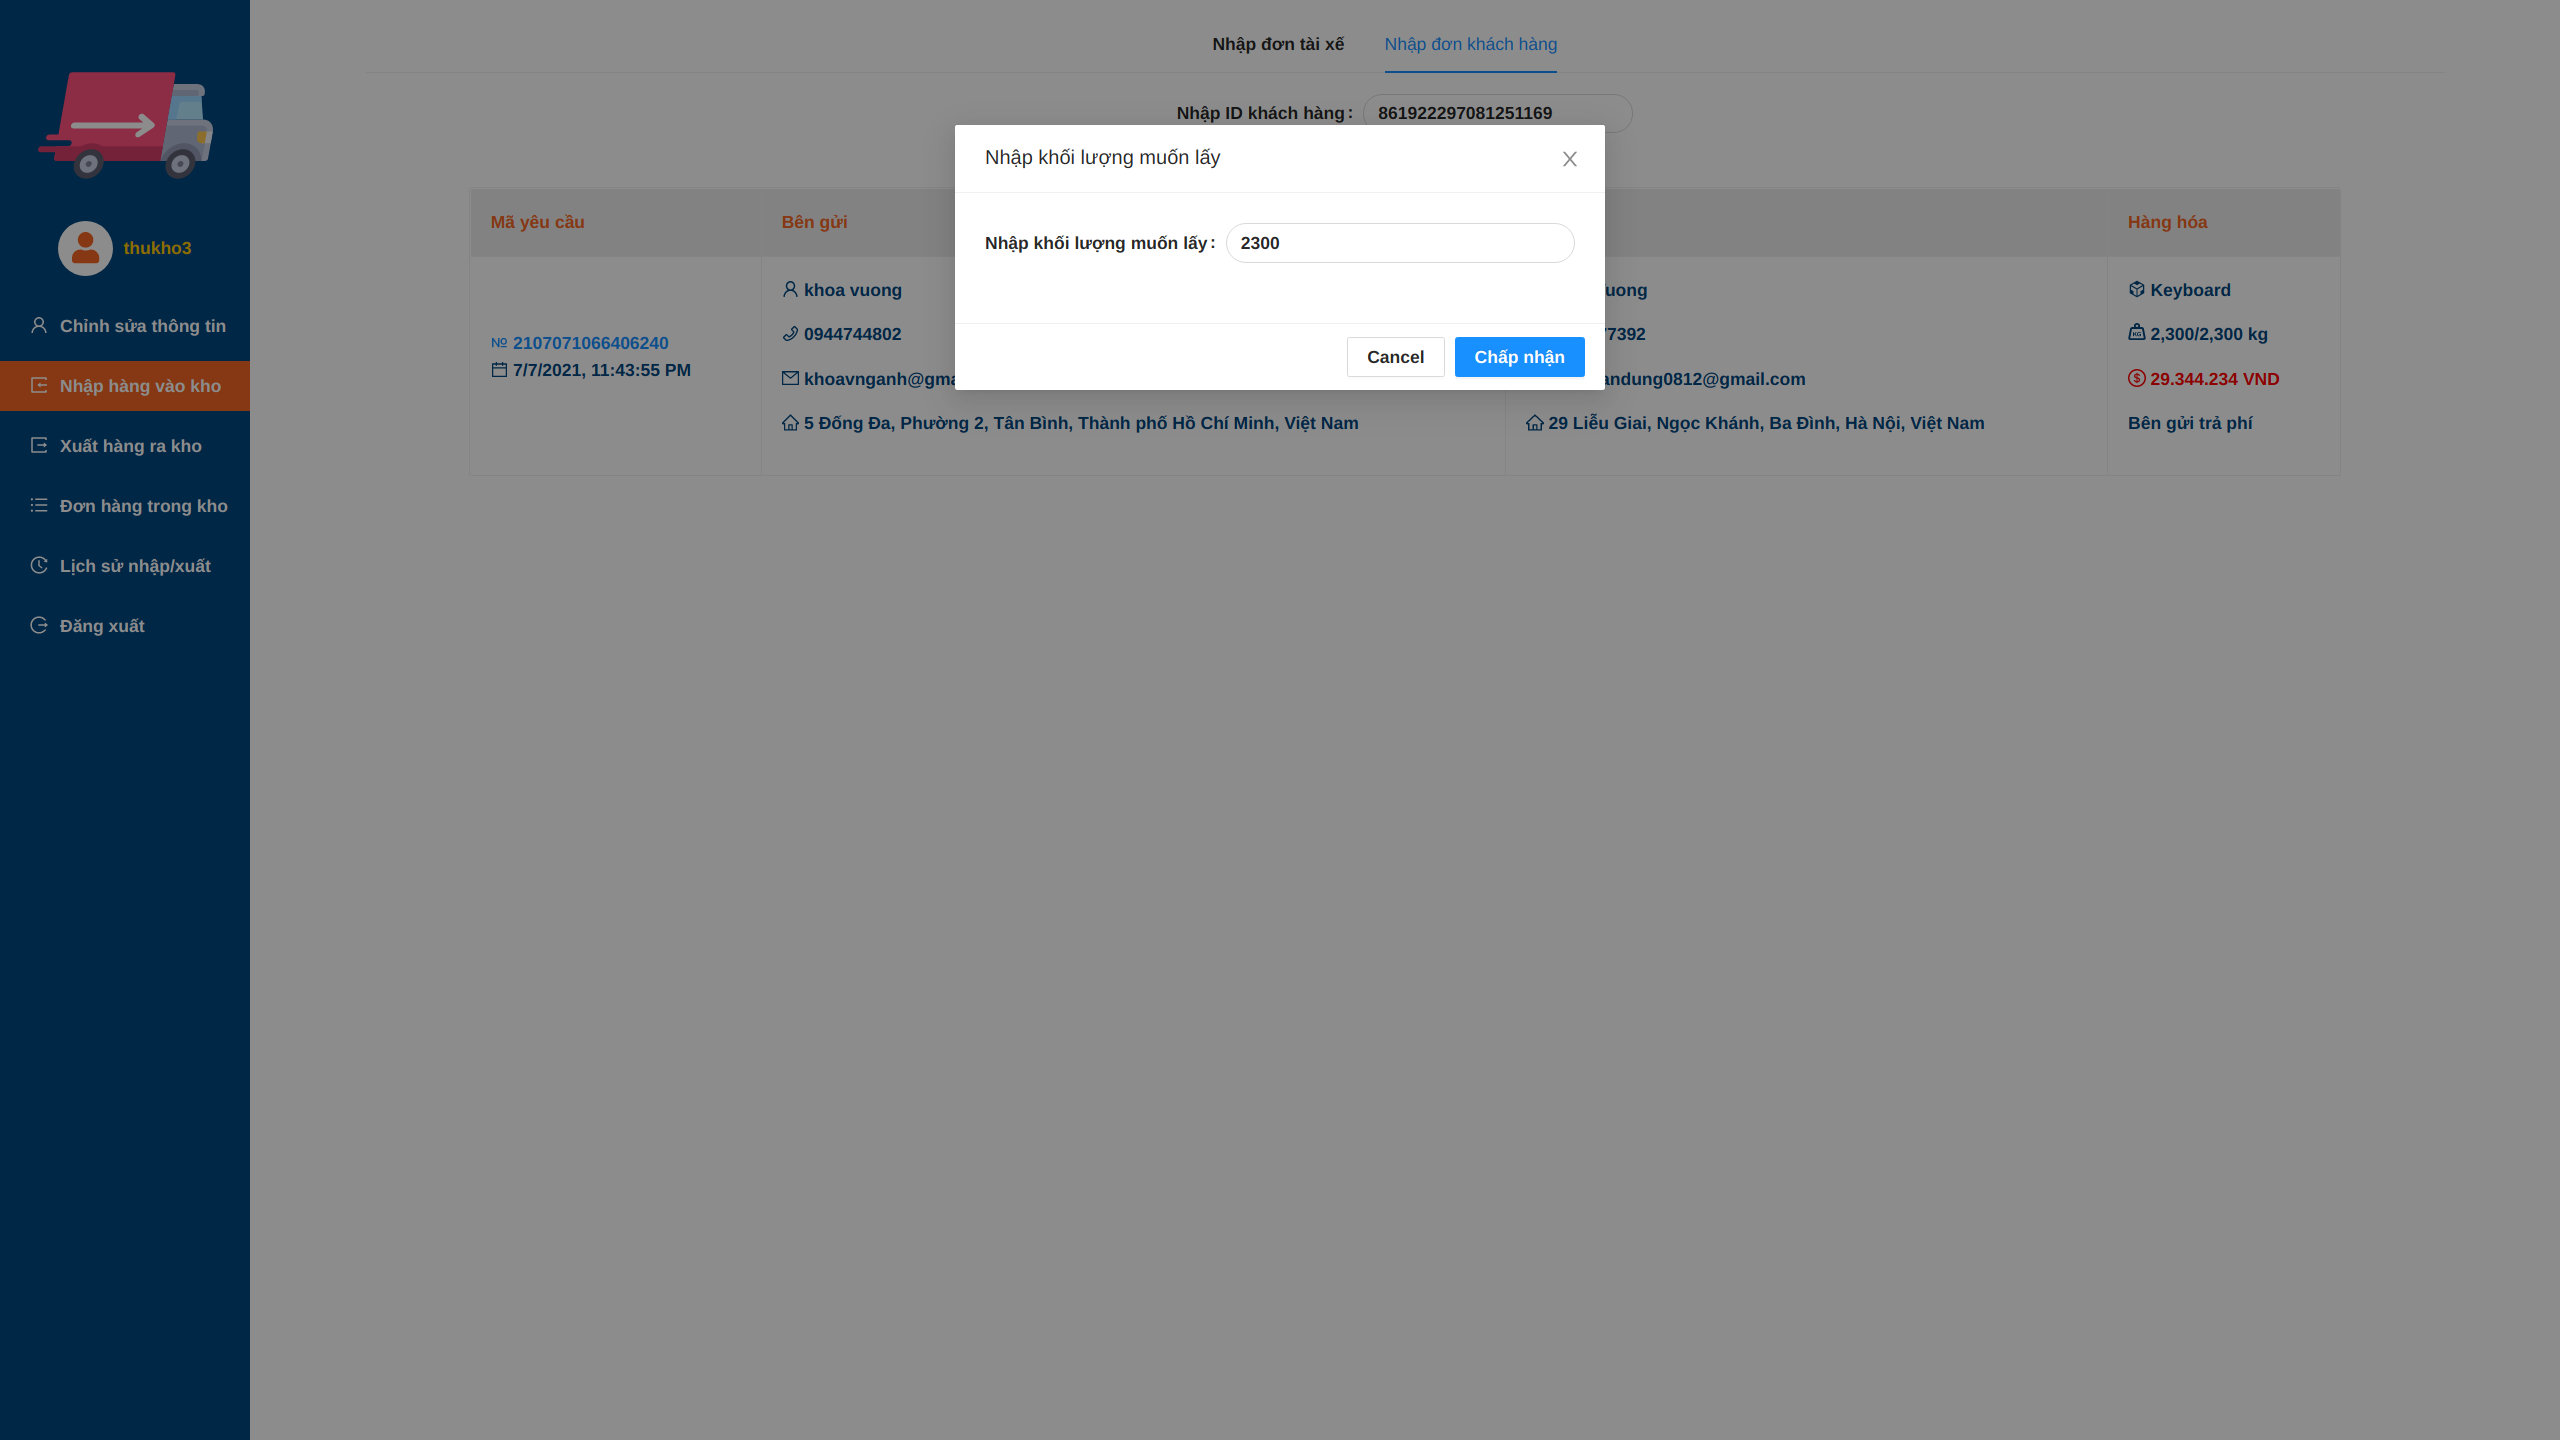
\includegraphics[width=1\textwidth]{/stockkeeper/stock_import_customer_detail.png}
		\centering
		\caption{Cho phép nhập khối lượng mà khách muốn nhập vào kho}
	\end{figure}
	
	\begin{figure}[H]
		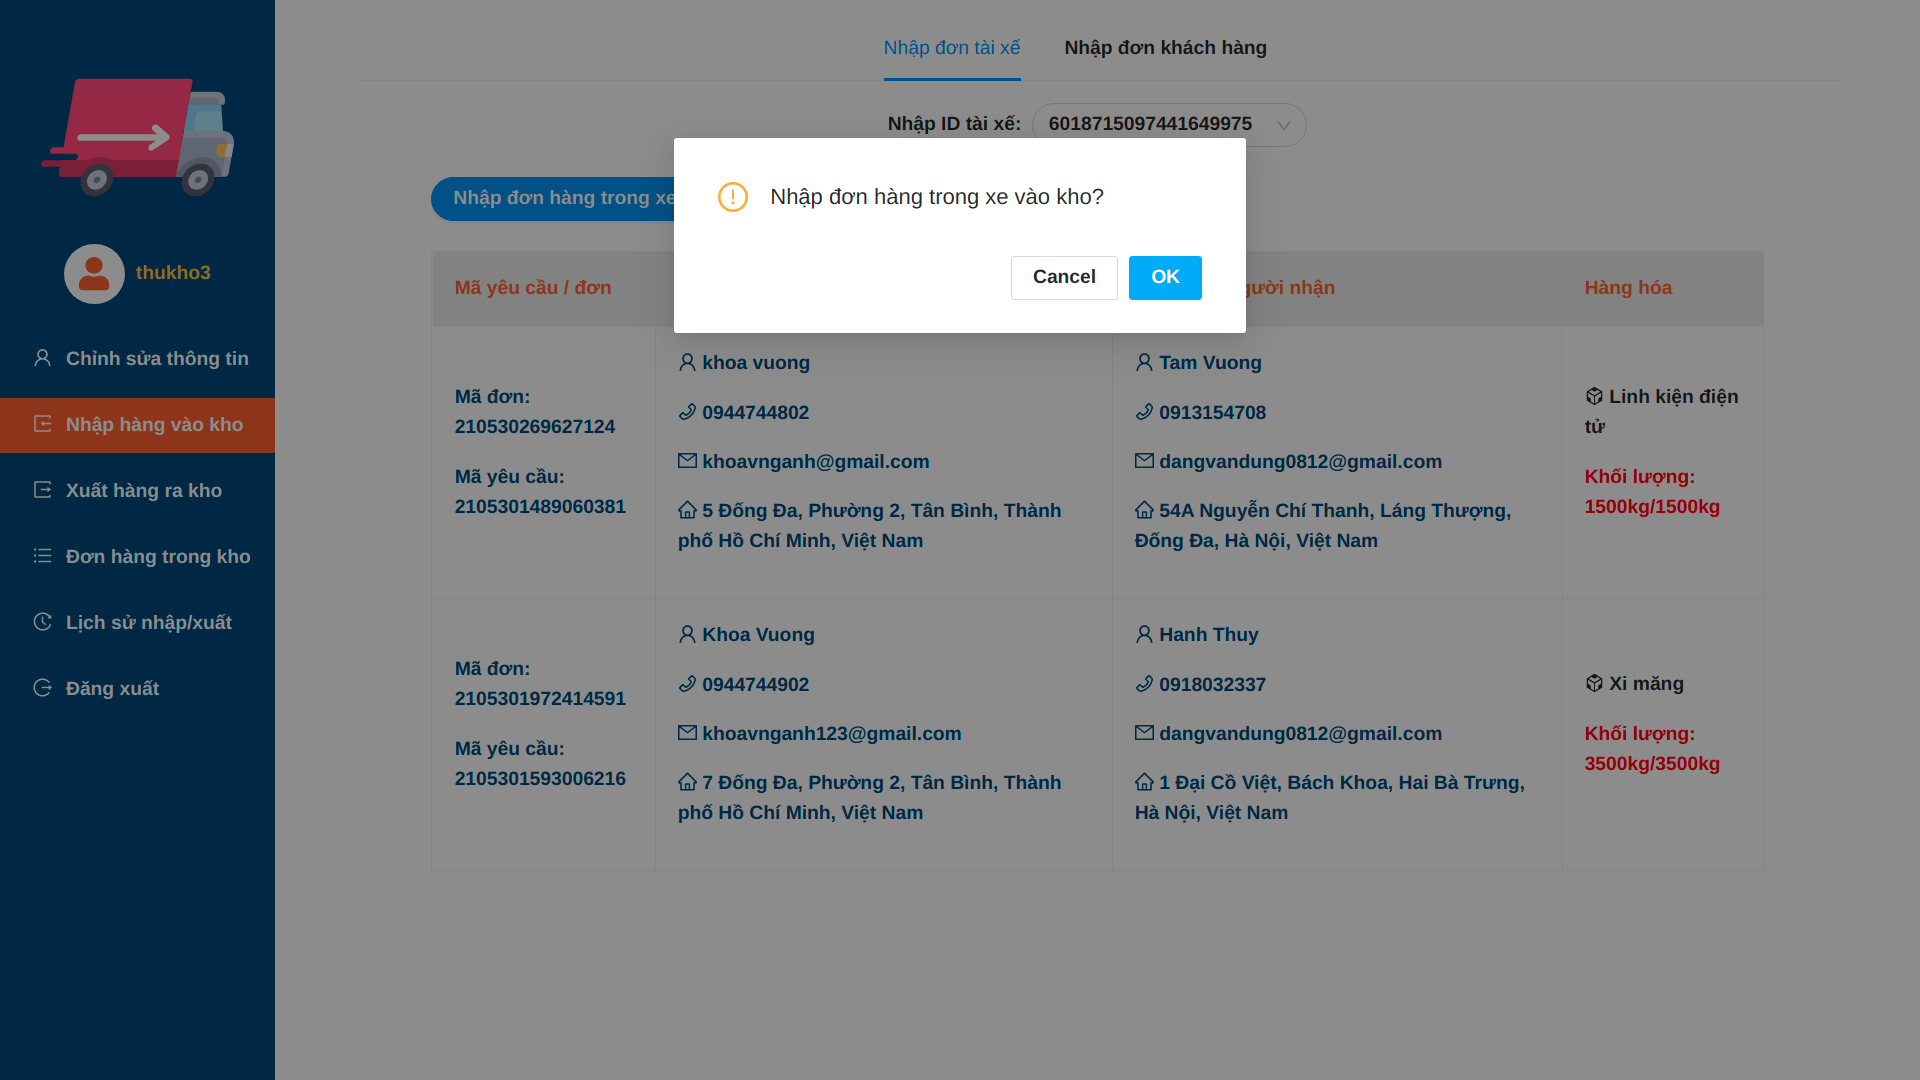
\includegraphics[width=1\textwidth]{/stockkeeper/stock_import_driver_prompt.png}
		\centering
		\caption{Xác nhận nhập hàng vào kho}
	\end{figure}
	
	\begin{figure}[H]
		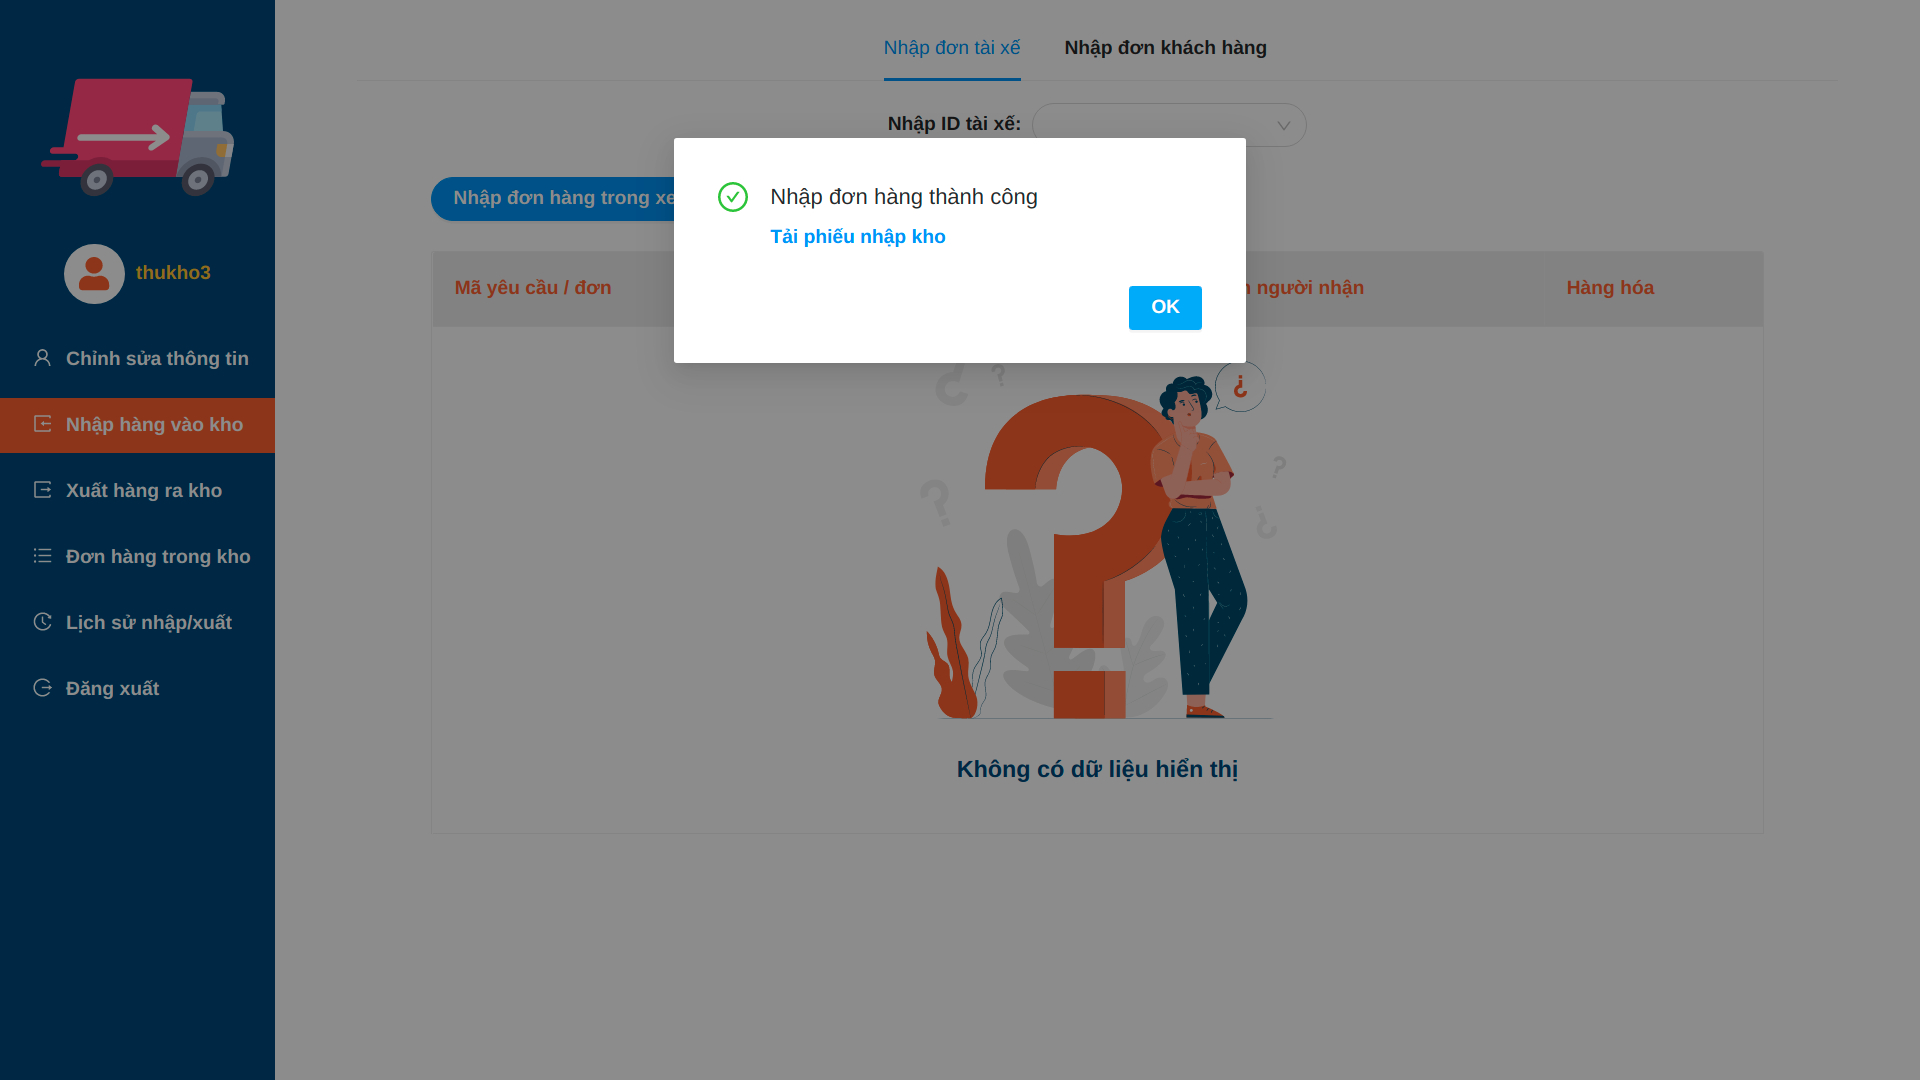
\includegraphics[width=1\textwidth]{/stockkeeper/stock_import_driver_pdf.png}
		\centering
		\caption{Nhập hàng thành công và cho thủ kho có thể tài phiếu nhập kho}
	\end{figure}

	\begin{figure}[H]
		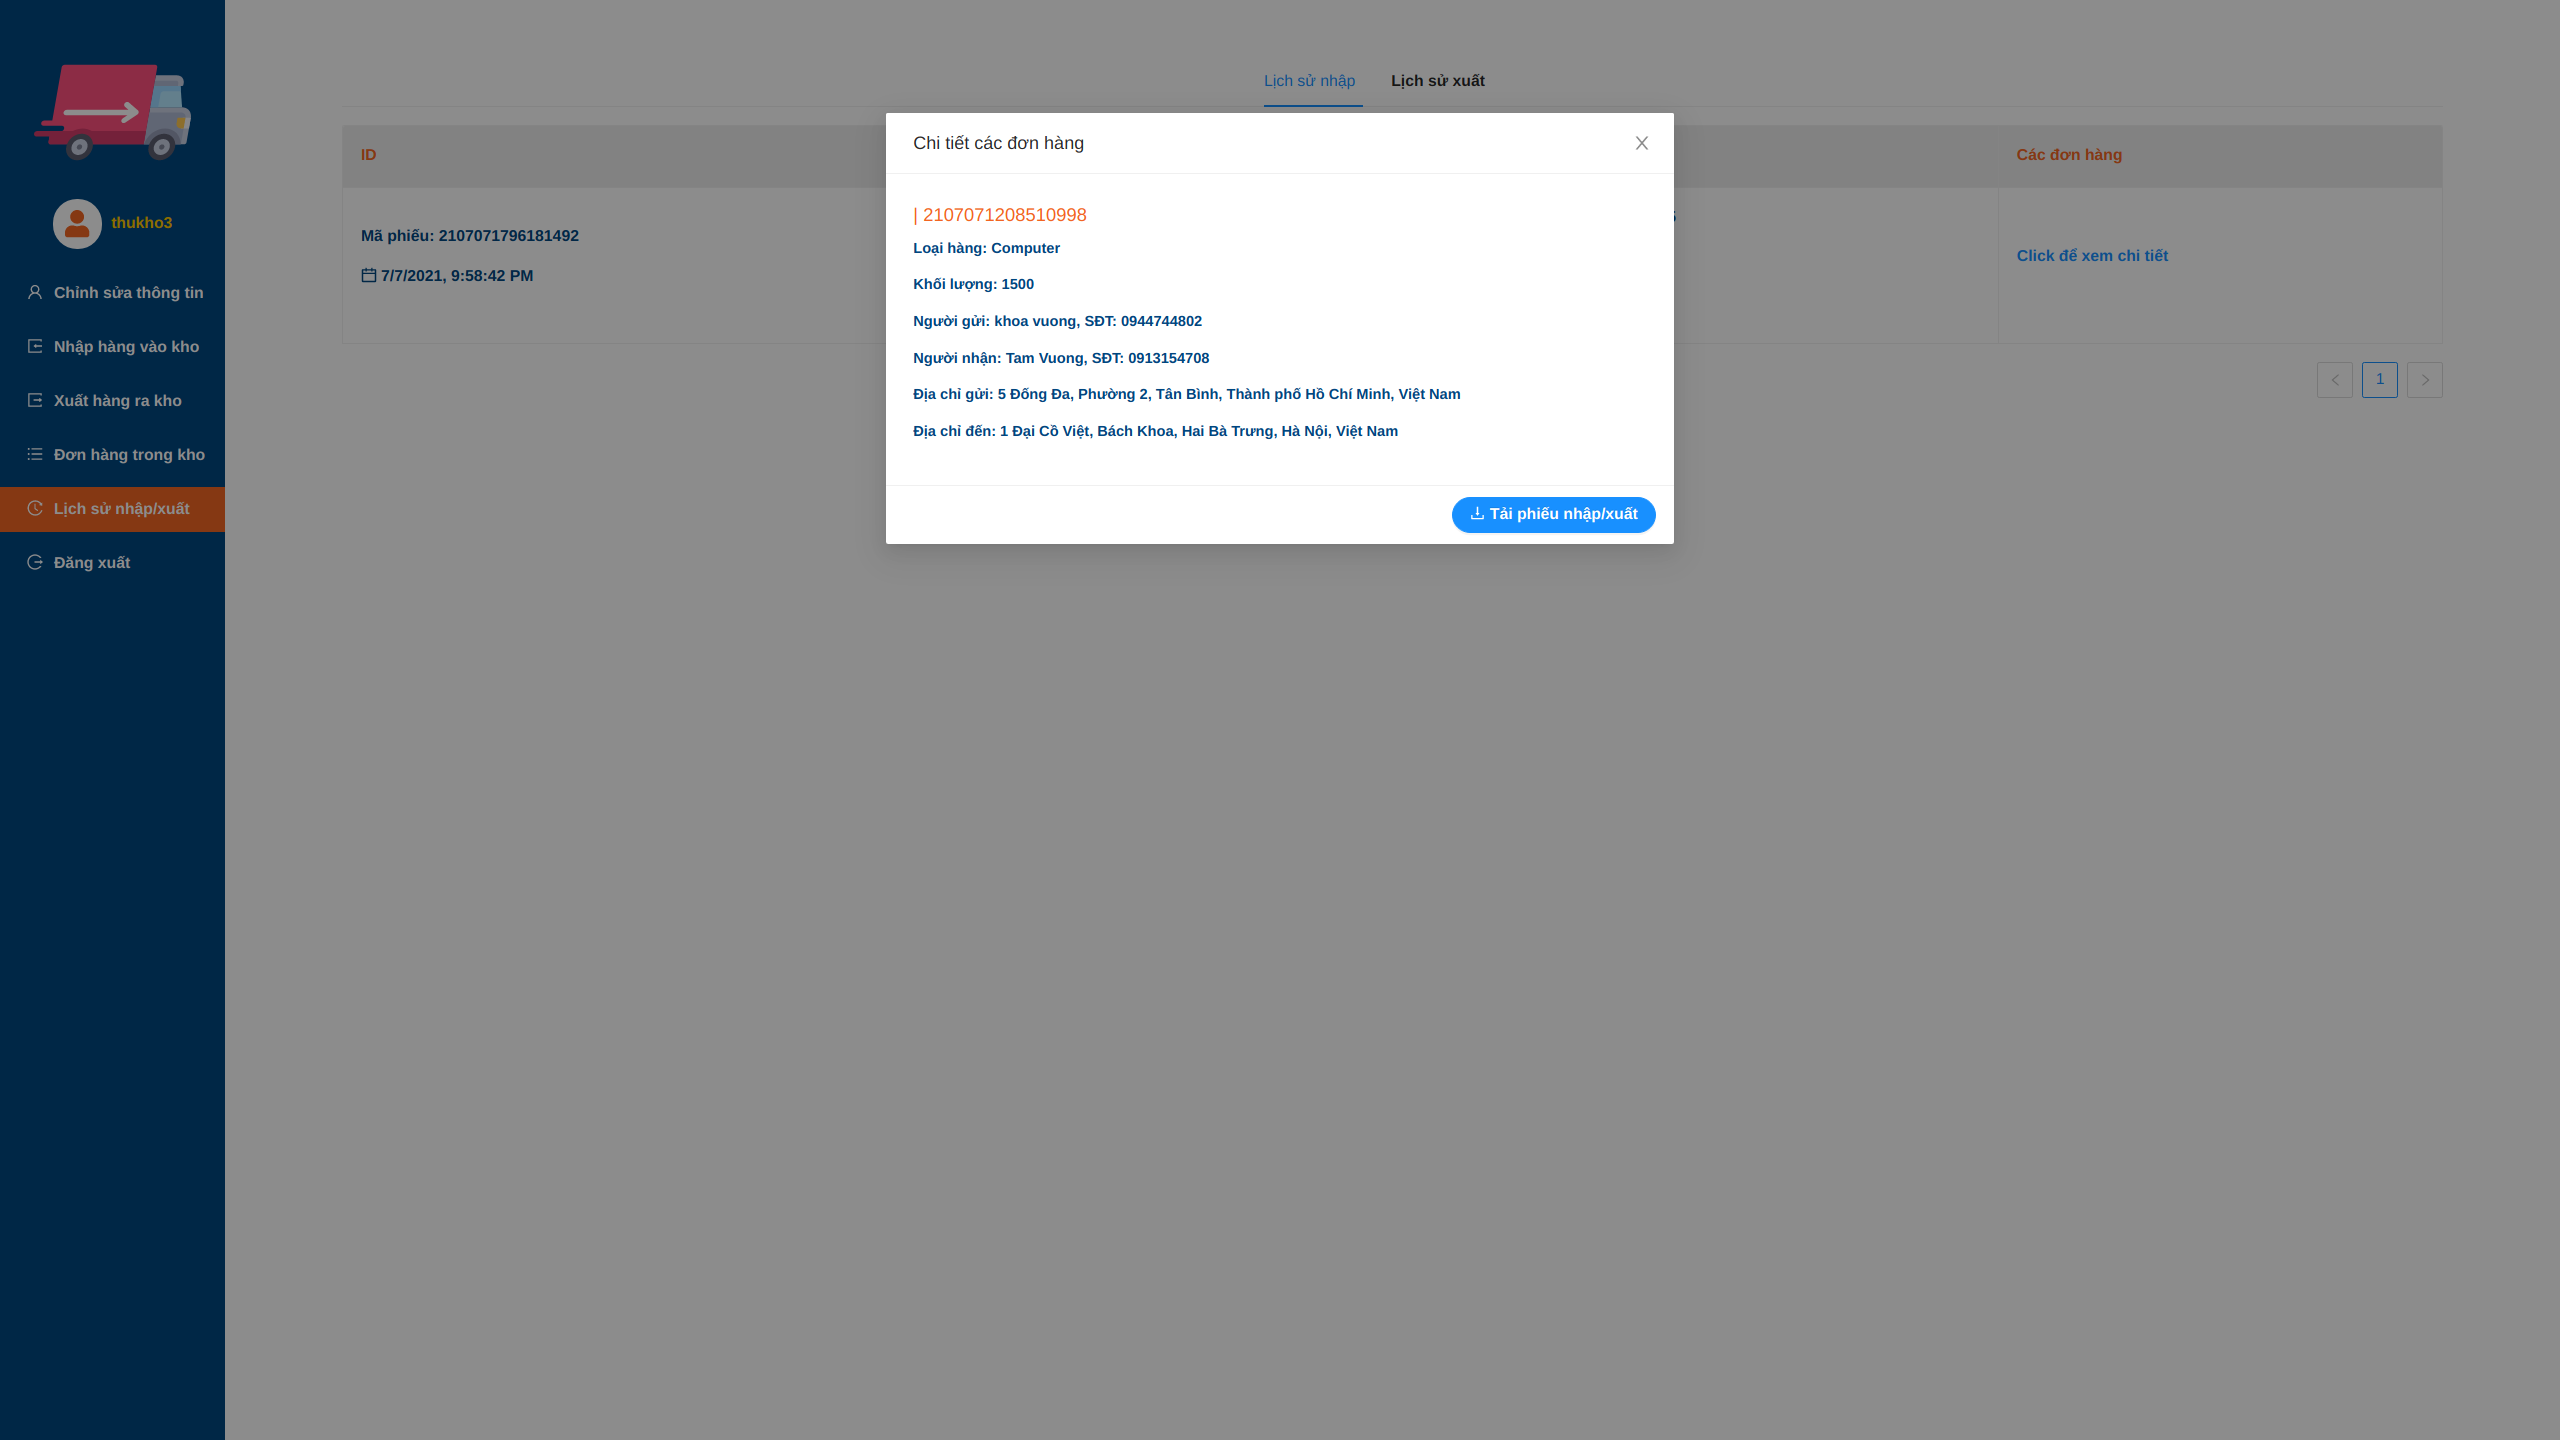
\includegraphics[width=1\textwidth]{/stockkeeper/stock_history_detail.png}
		\centering
		\caption{Thông tin chi tiết của một lần nhập/xuất đơn hàng (Cho phép tải pdf về)}
	\end{figure}
	
	\begin{figure}[H]
		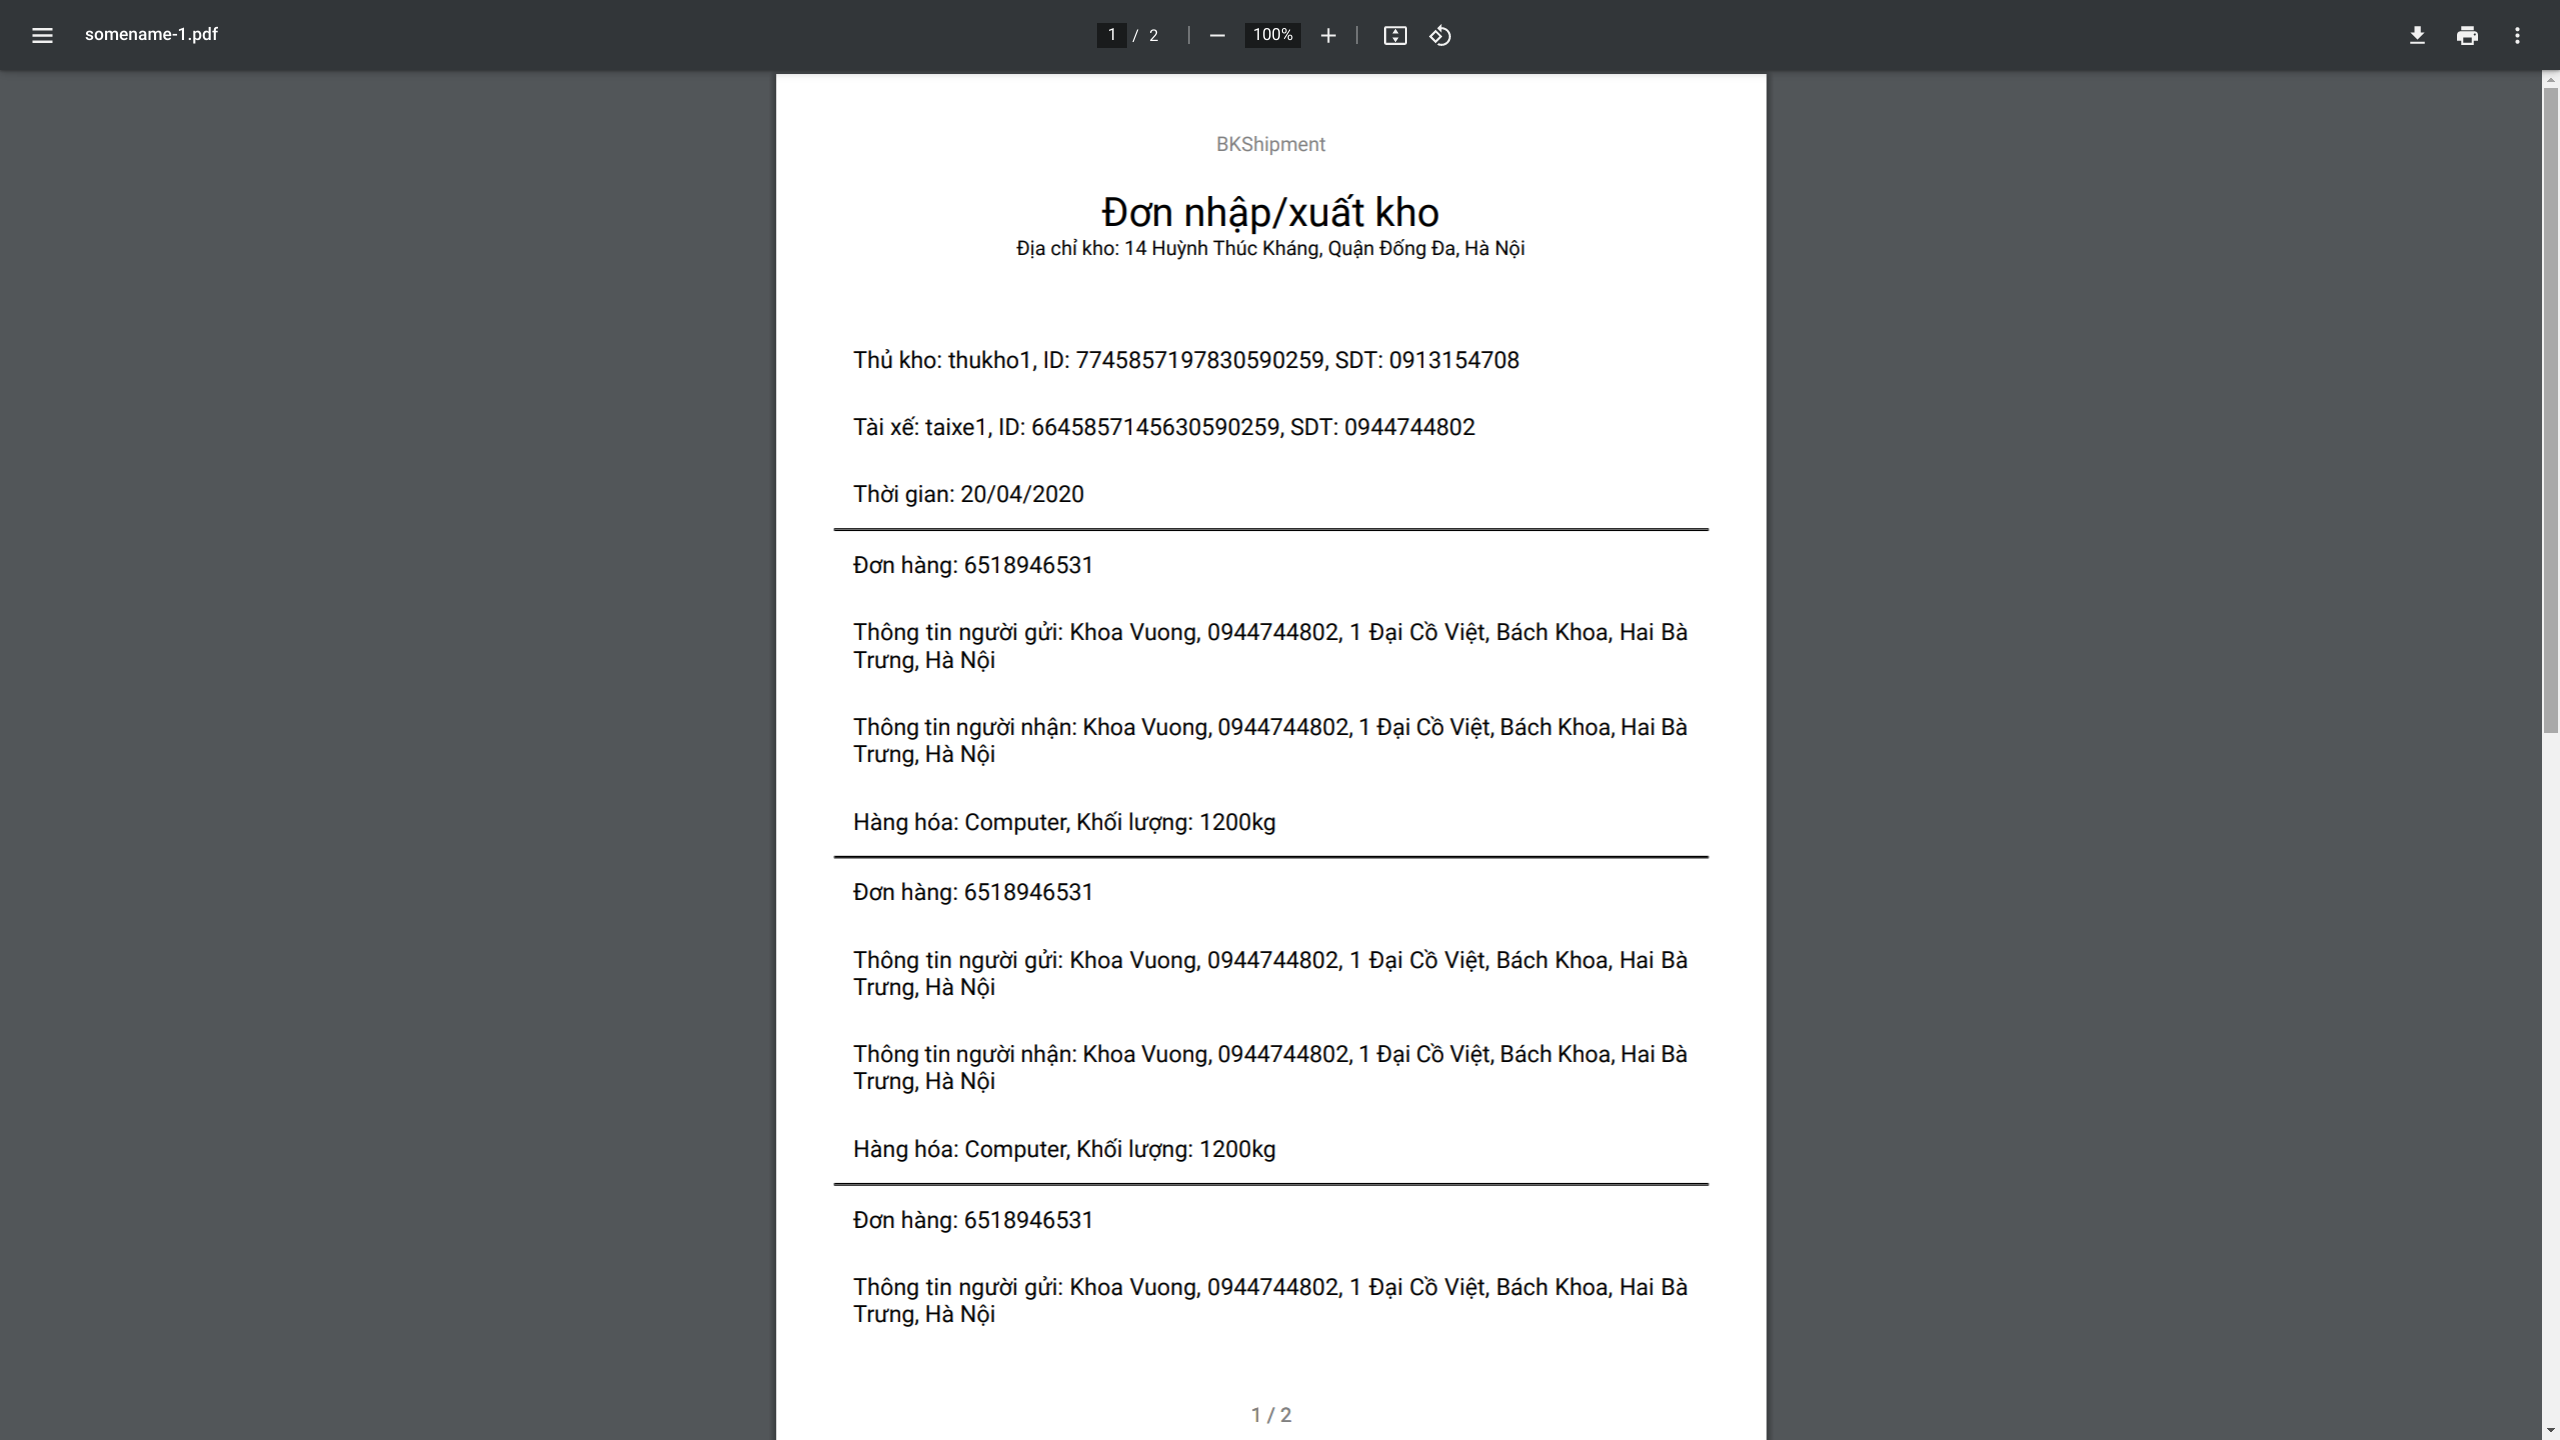
\includegraphics[width=1\textwidth]{/stockkeeper/stock_pdf.png}
		\centering
		\caption{Format mẫu của 1 đơn nhập/xuất kho}
	\end{figure}
	
	
	\item \textbf{Xem danh sách đơn hàng}
	\begin{figure}[H]
		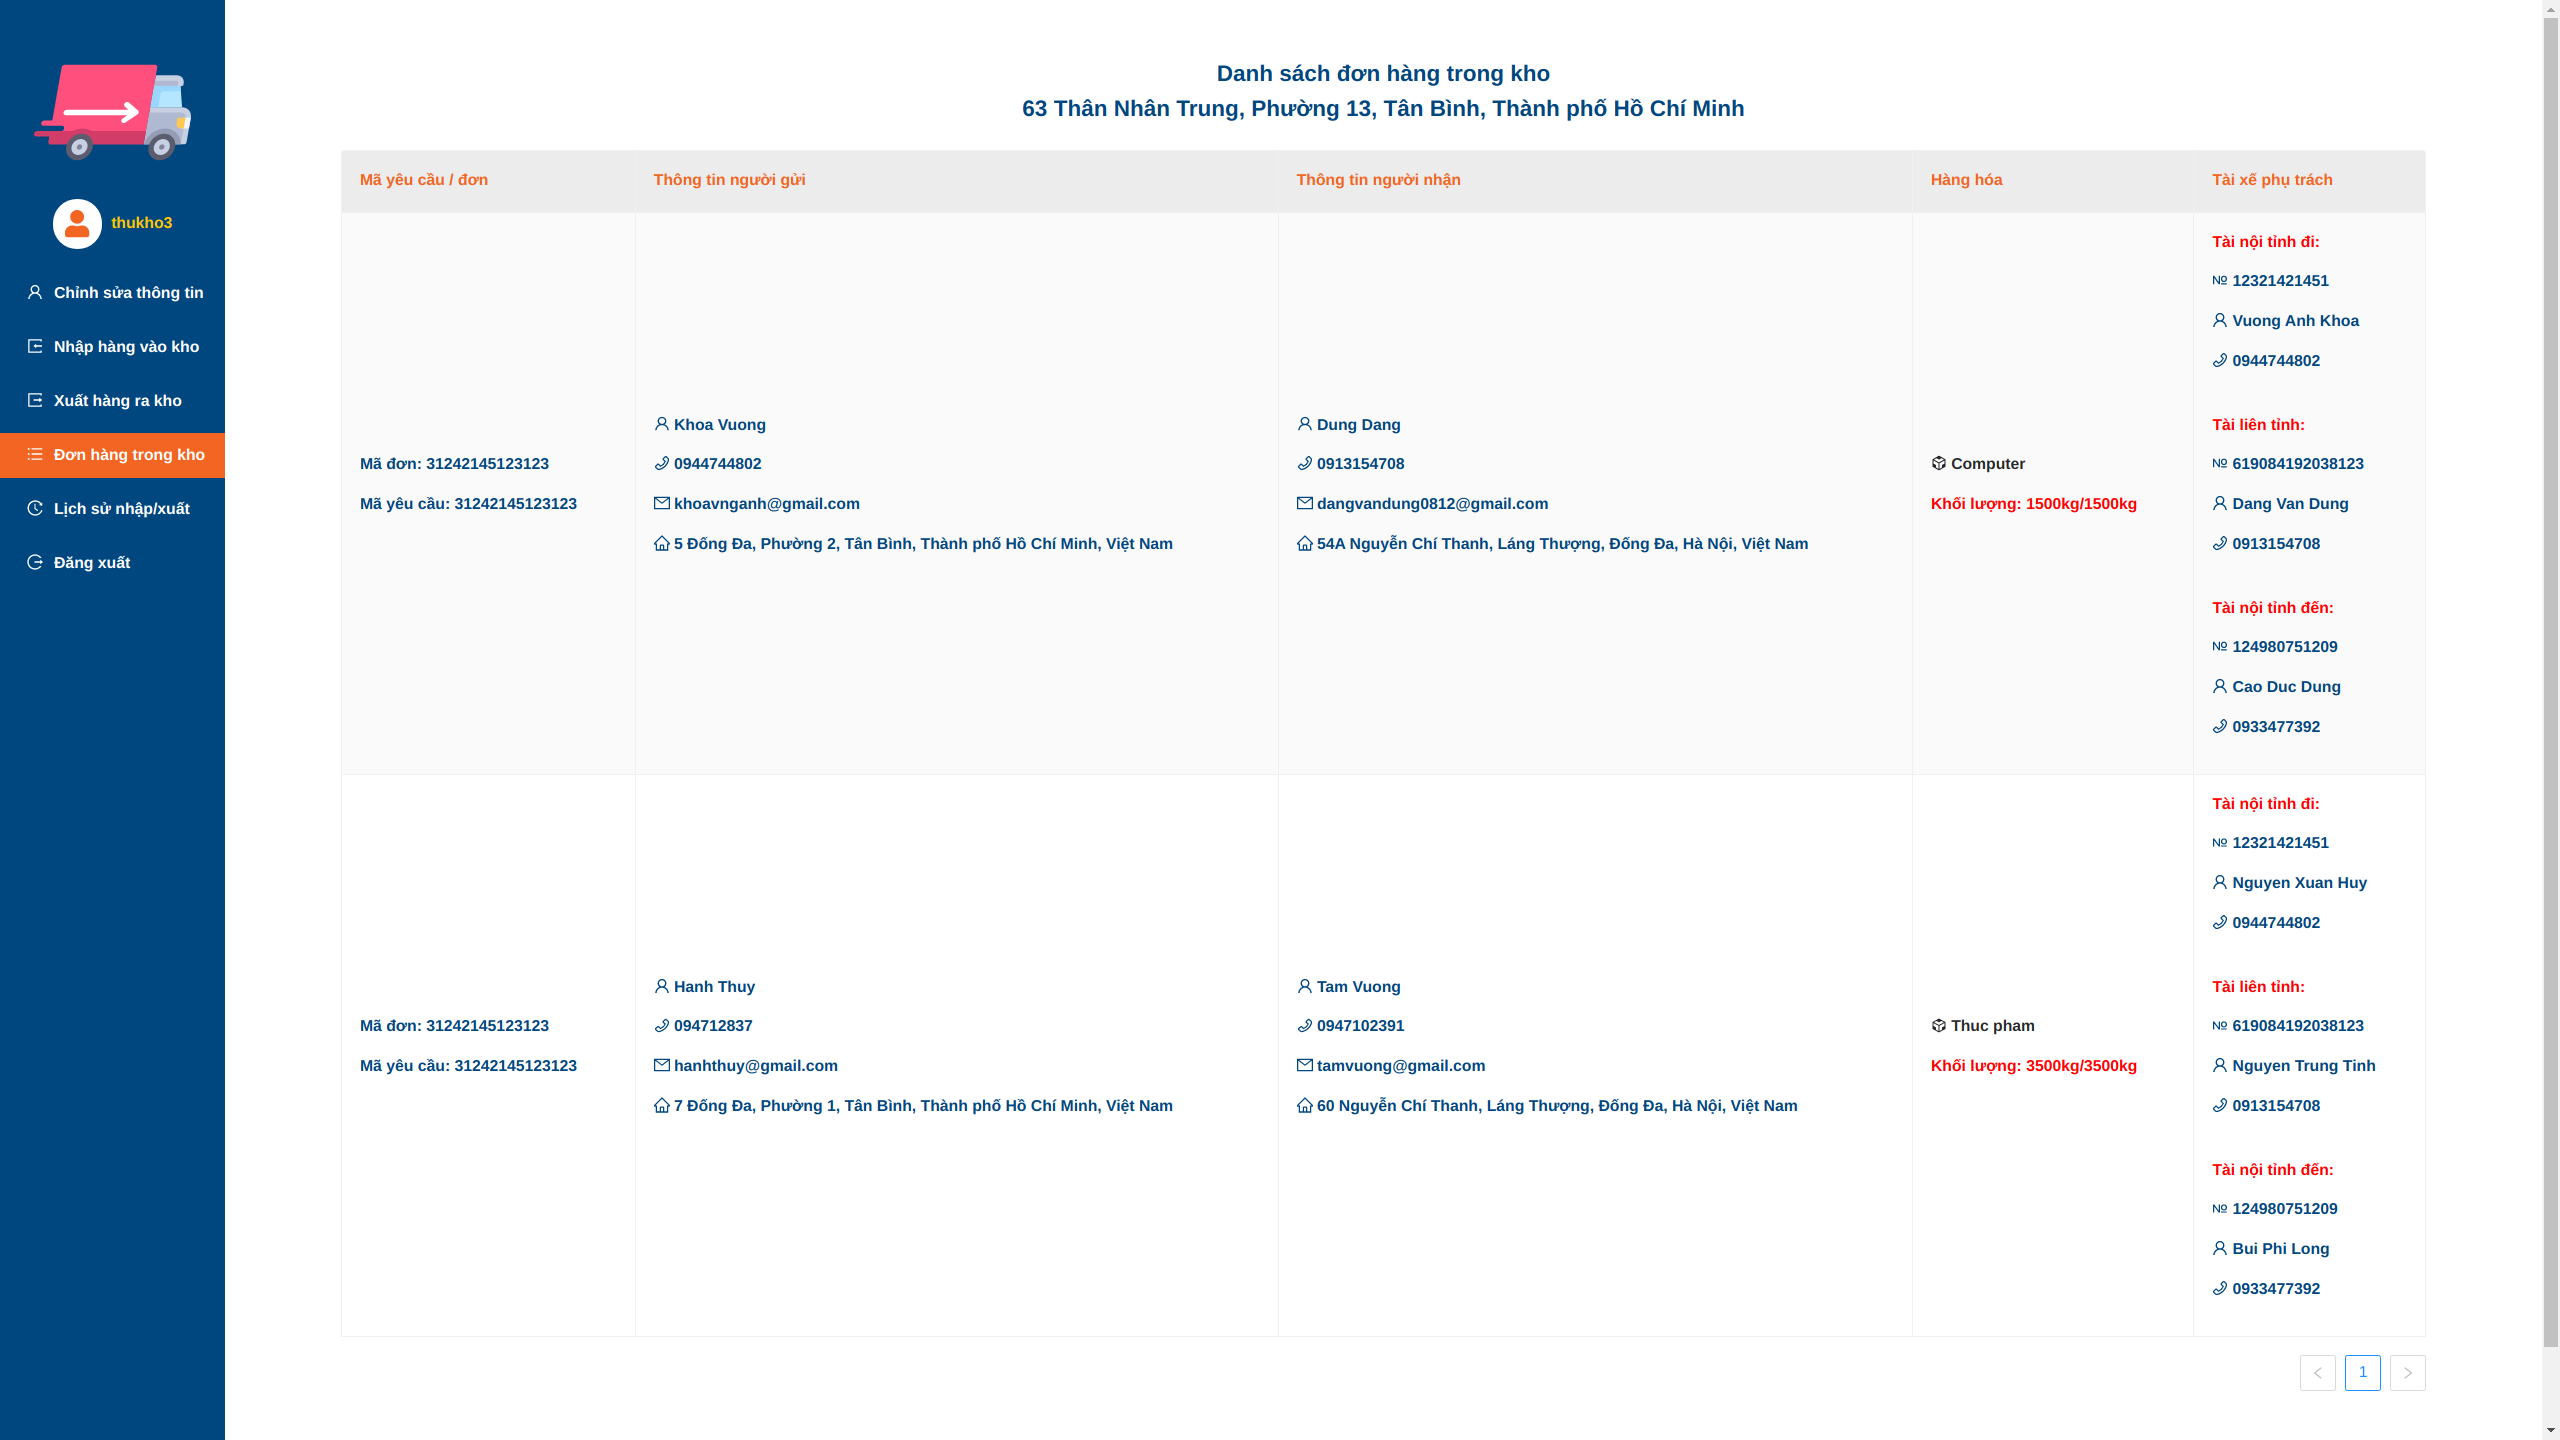
\includegraphics[width=1\textwidth]{/stockkeeper/stock_list.png}
		\centering
		\caption{Danh sách các đơn hàng trong kho}
	\end{figure}

	\begin{figure}[H]
		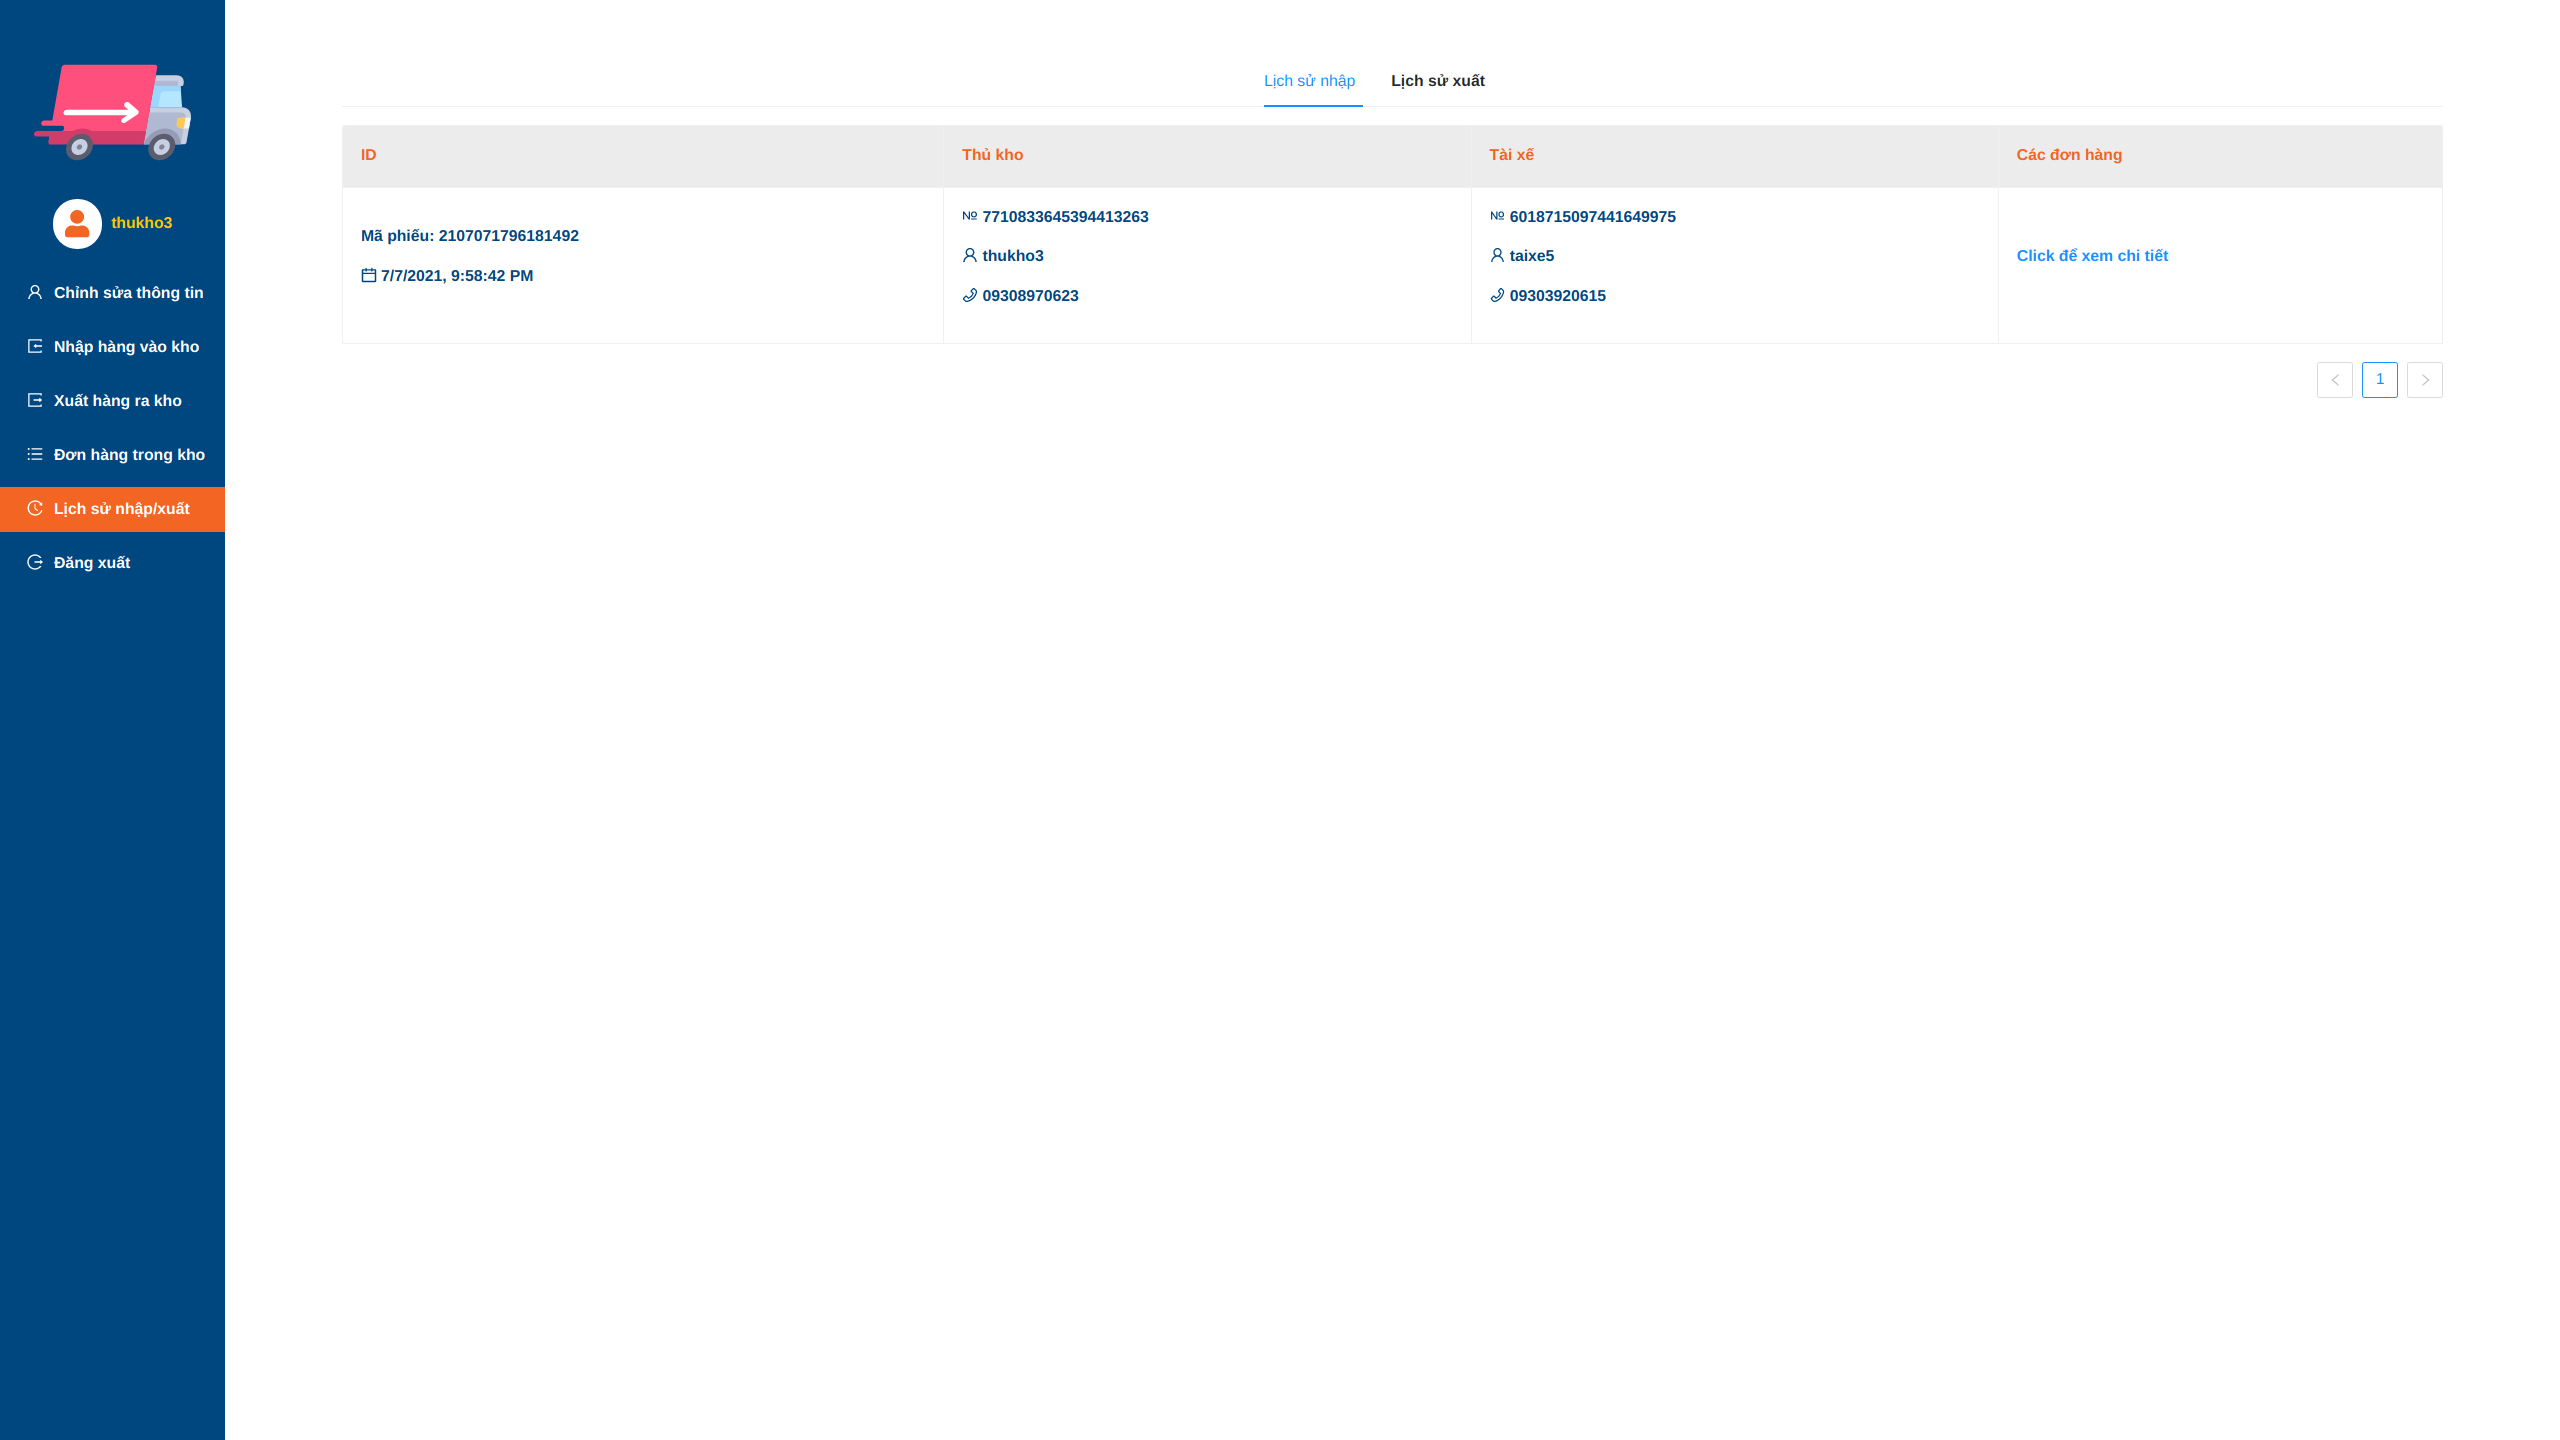
\includegraphics[width=1\textwidth]{/stockkeeper/stock_history.png}
		\centering
		\caption{Lịch sử nhập/xuất kho}
	\end{figure}
	
	Chức năng xuất kho có giao diện và tính năng tương tự lúc nhập kho.
	
\end{itemize}

\subsection{Chức năng dành cho Quản lý}
\begin{itemize}
	\item \textbf{Quản lý tài xế}
	\begin{figure}[H]
		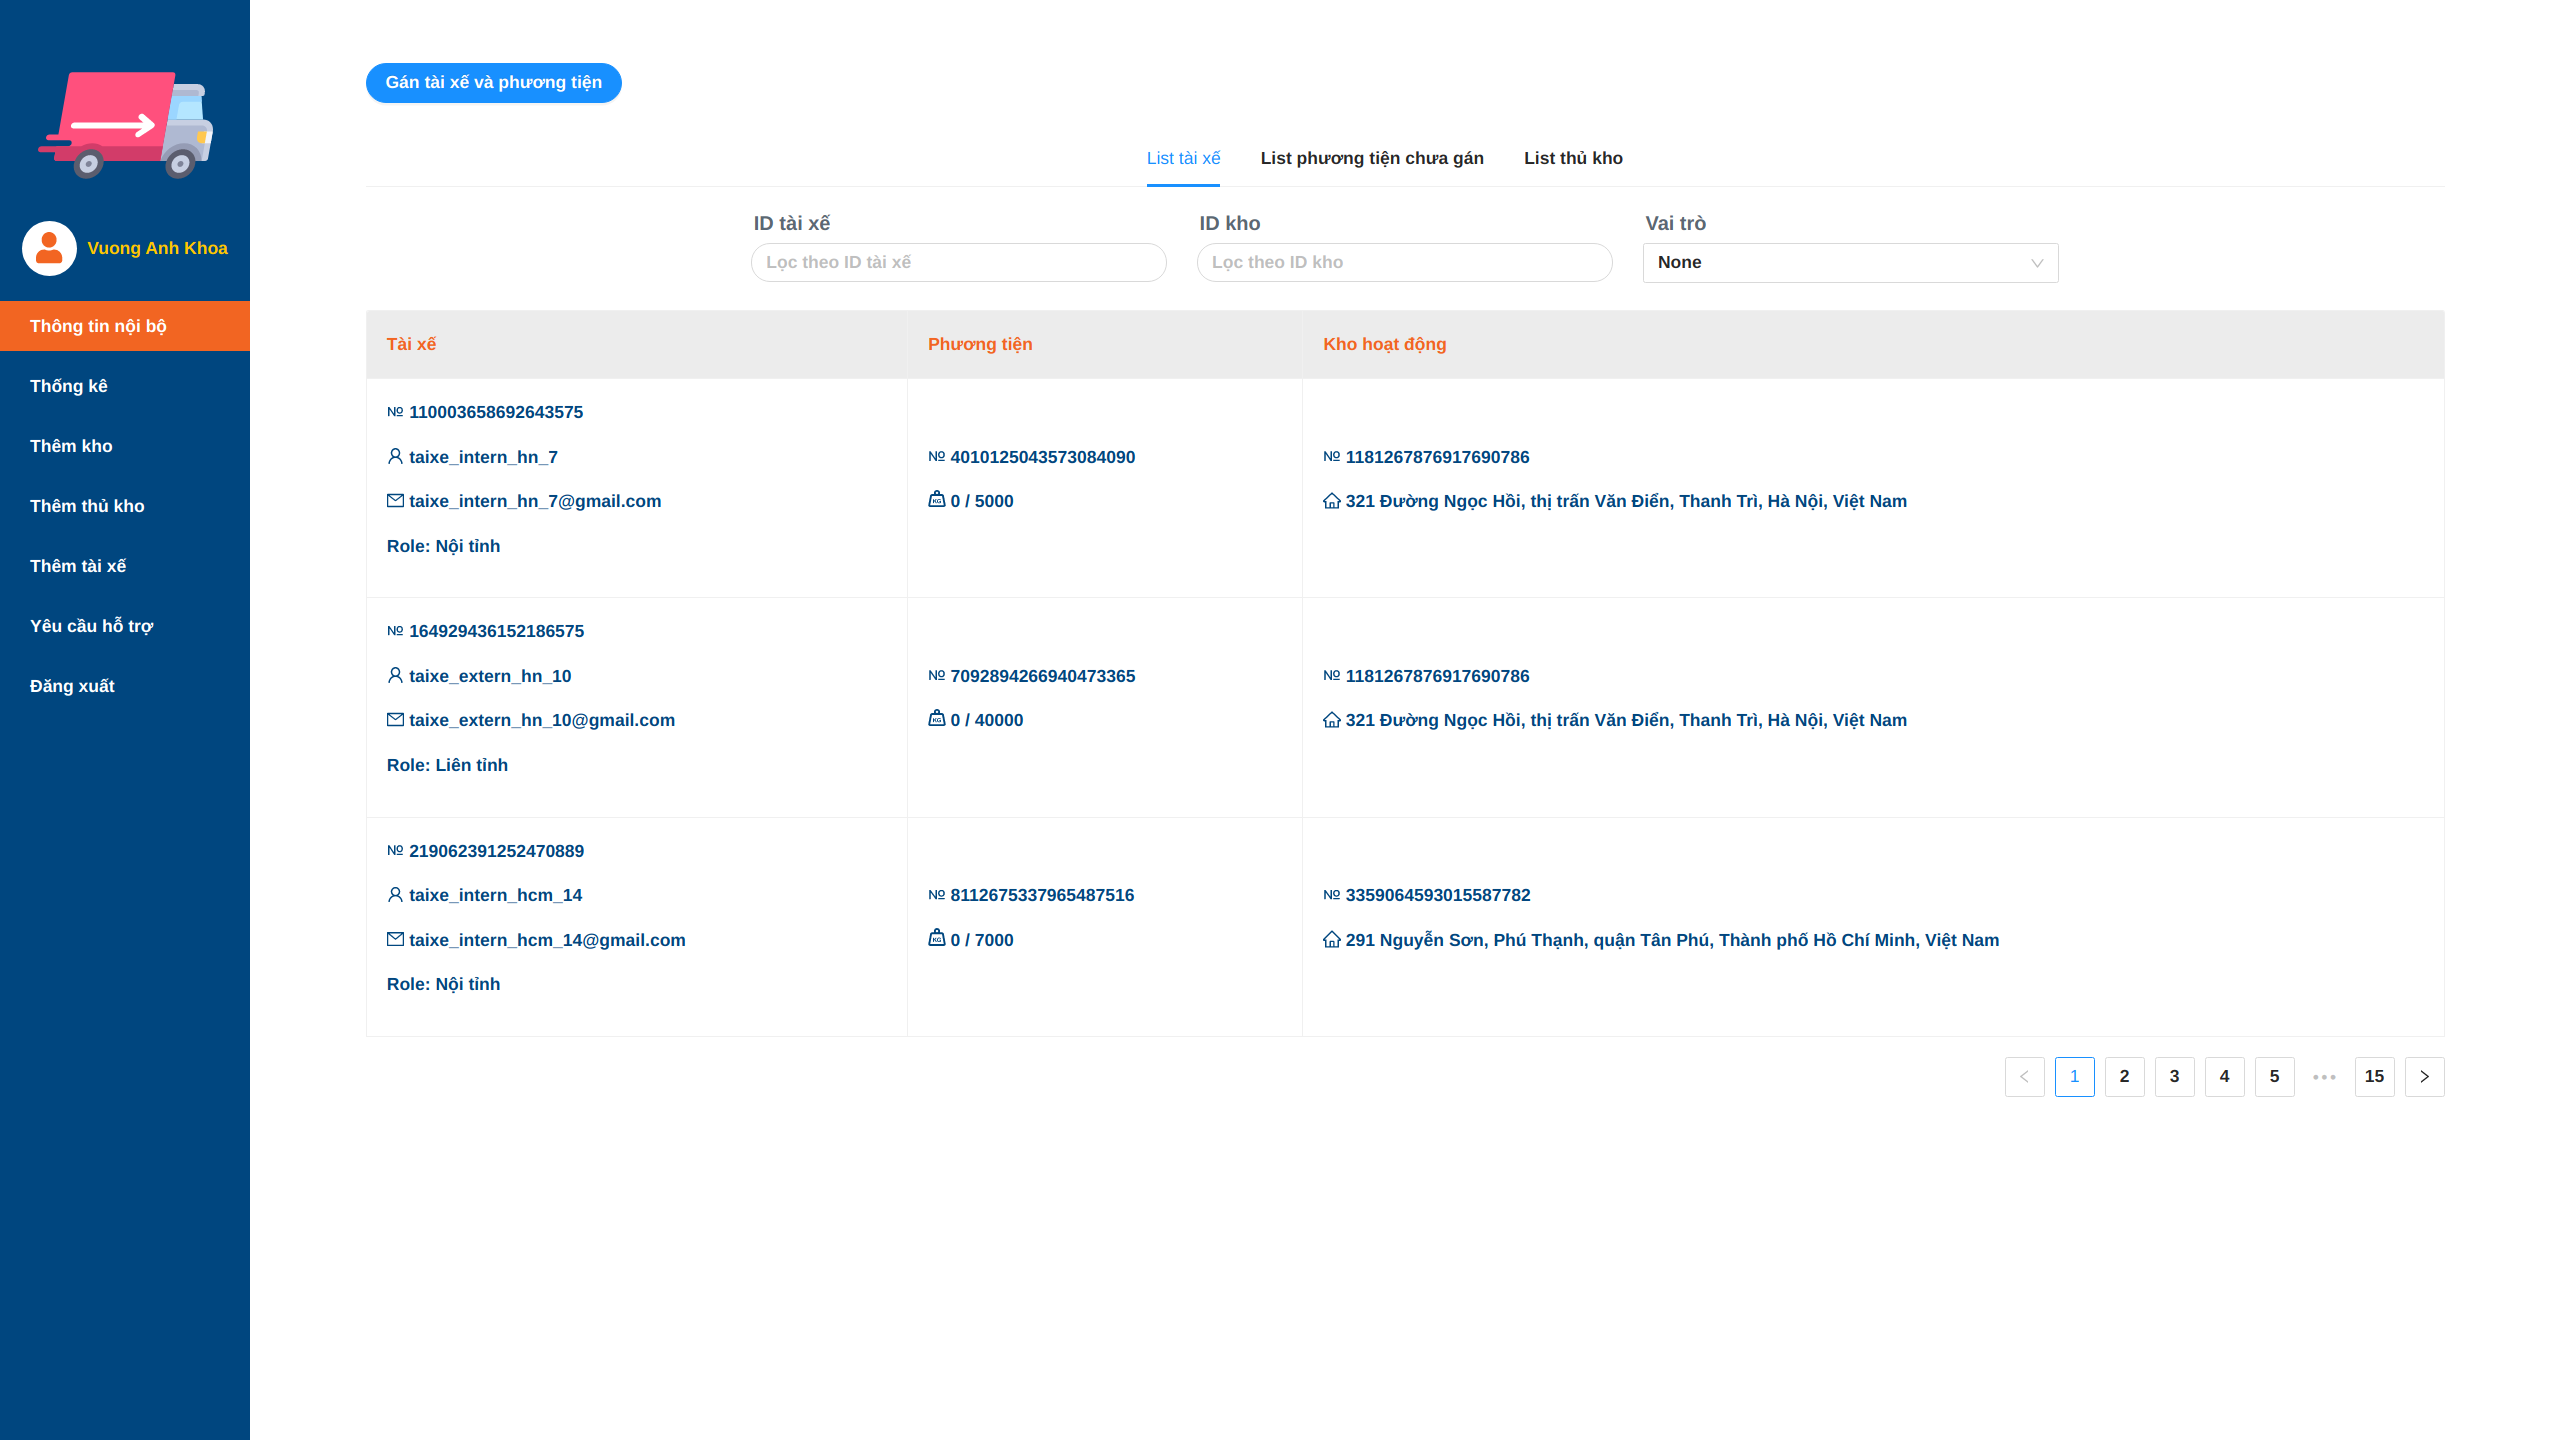
\includegraphics[width=1\textwidth]{/admin/admin_list_driver.png}
		\centering
		\caption{Xem danh sách các tài xế trong hệ thống}
	\end{figure}
	
	
	\item \textbf{Quản lý thủ kho}
	\begin{figure}[H]
		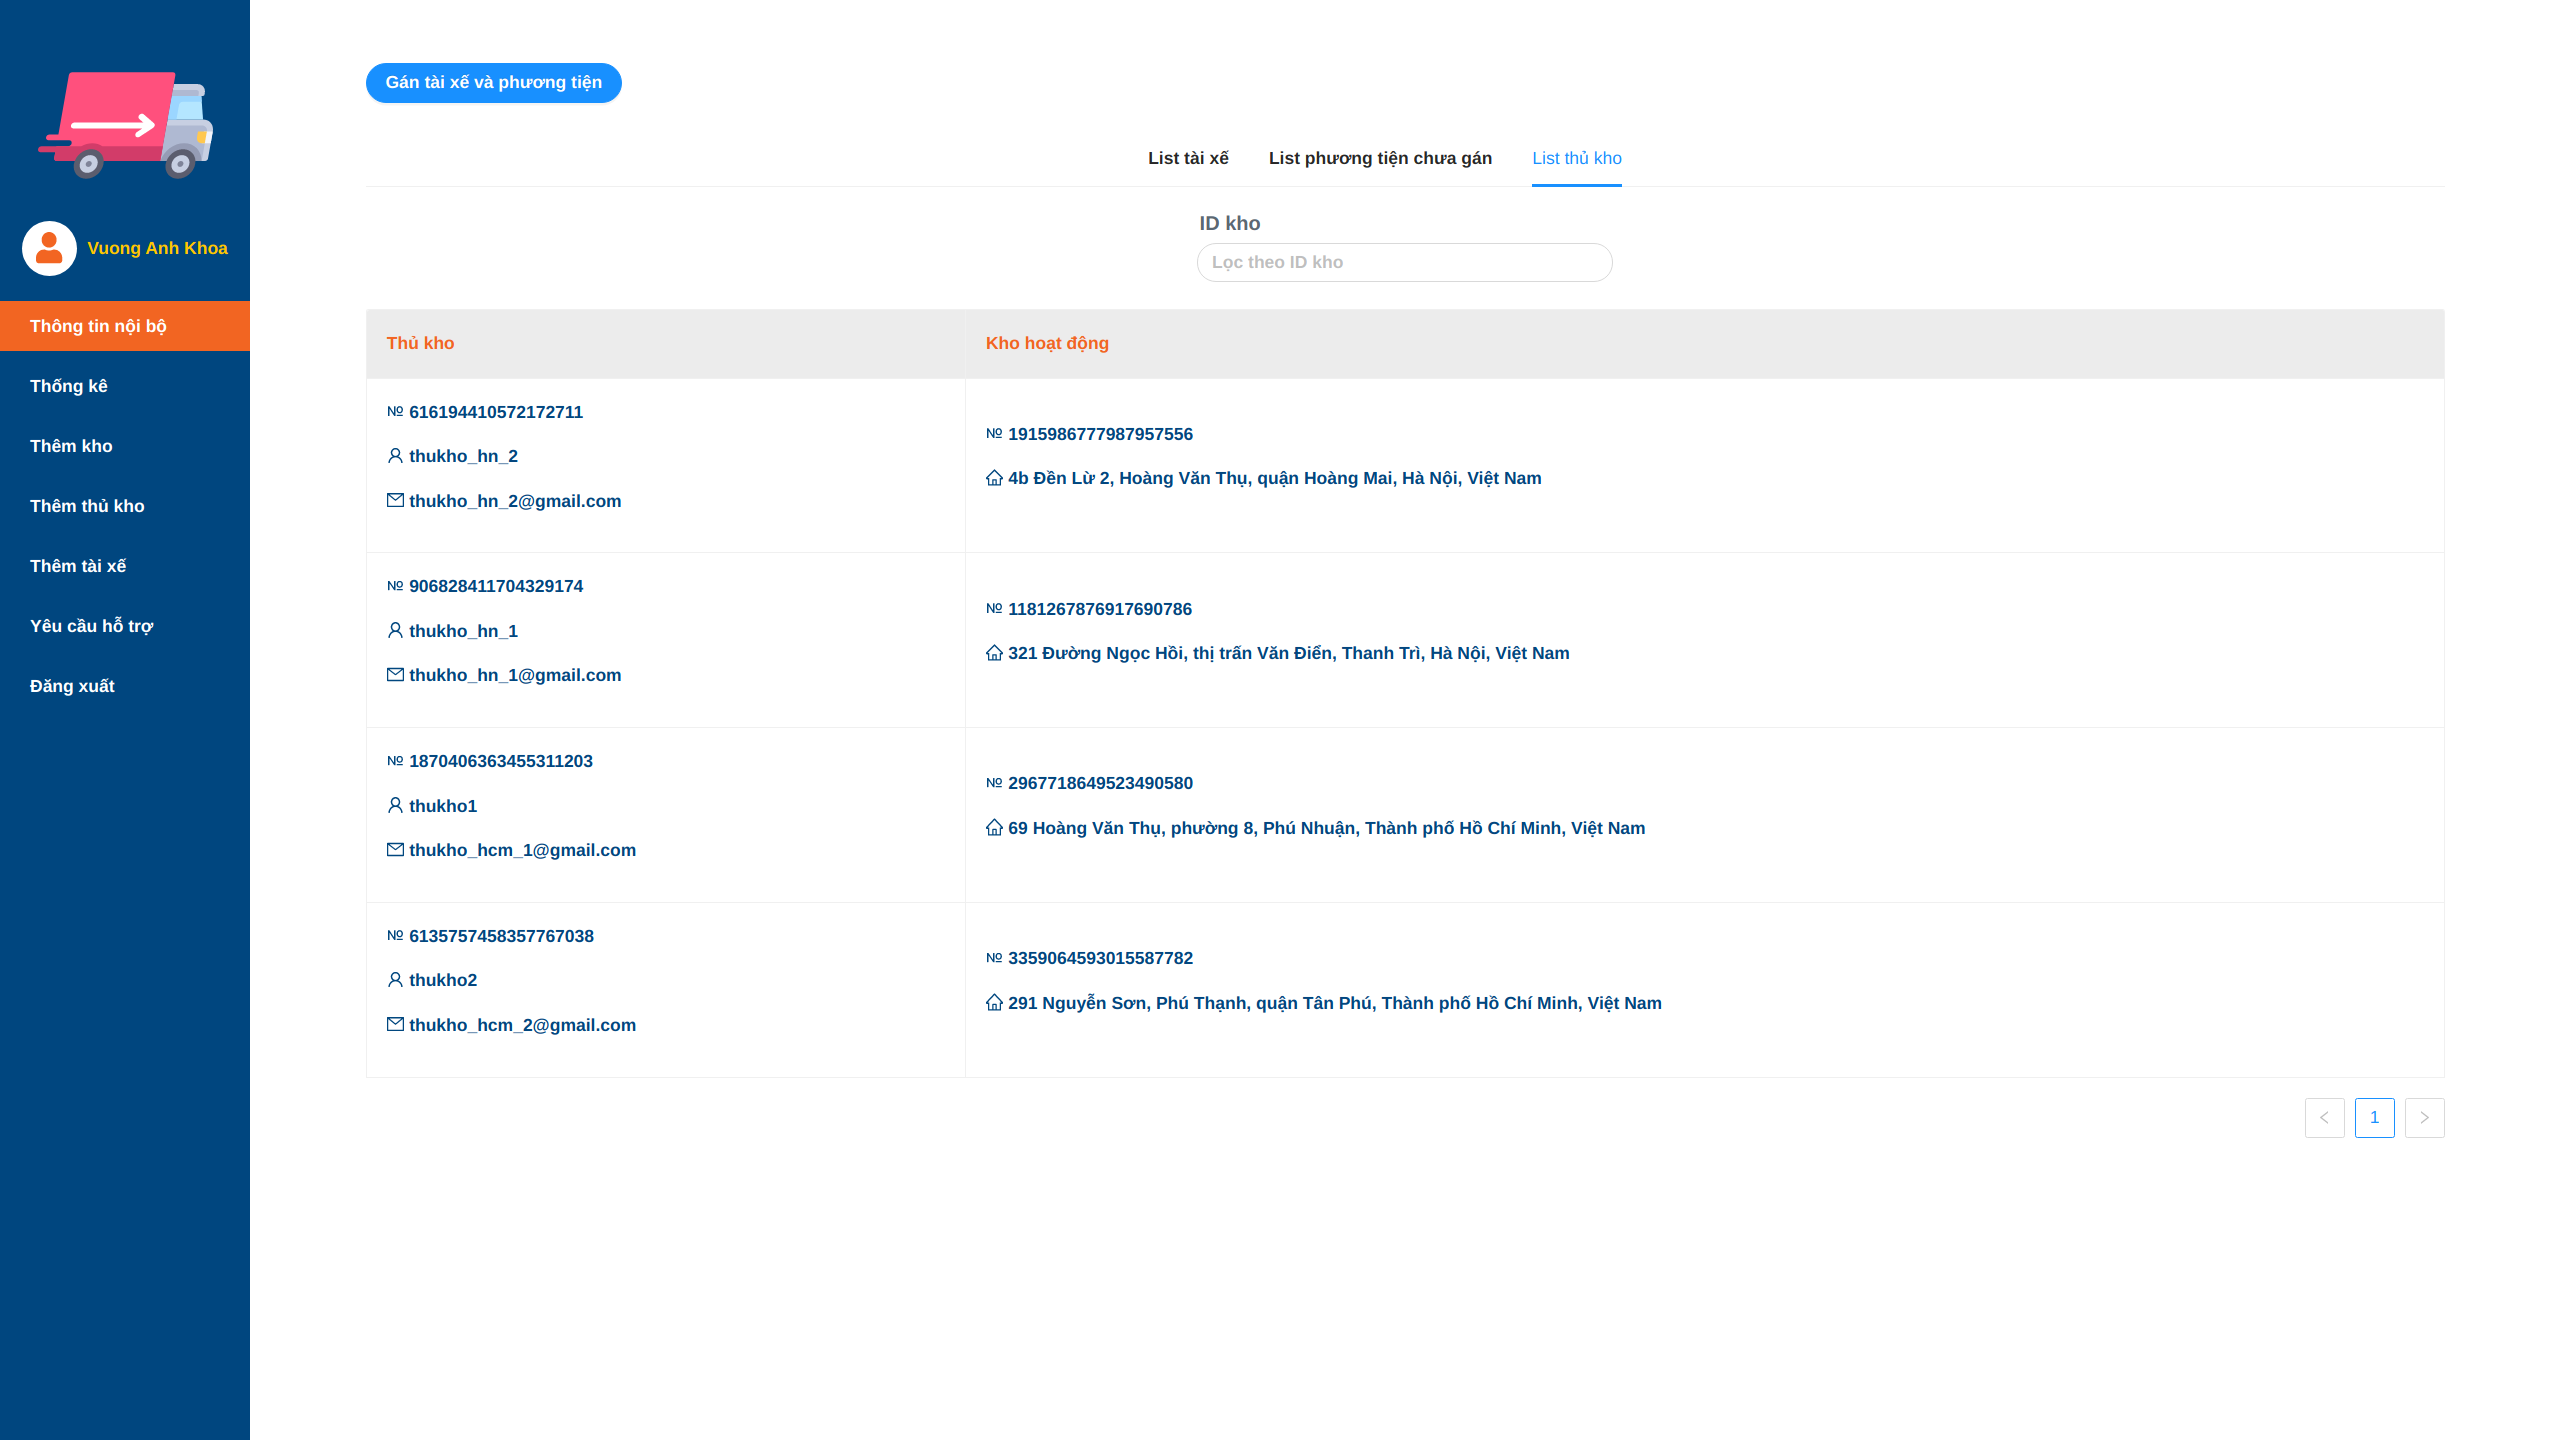
\includegraphics[width=1\textwidth]{/admin/admin_list_stock.png}
		\centering
		\caption{Xem danh sách các kho và thủ kho phụ trách của hệ thống}
	\end{figure}

	\item \textbf{Xem thống kê}
	\begin{figure}[H]
		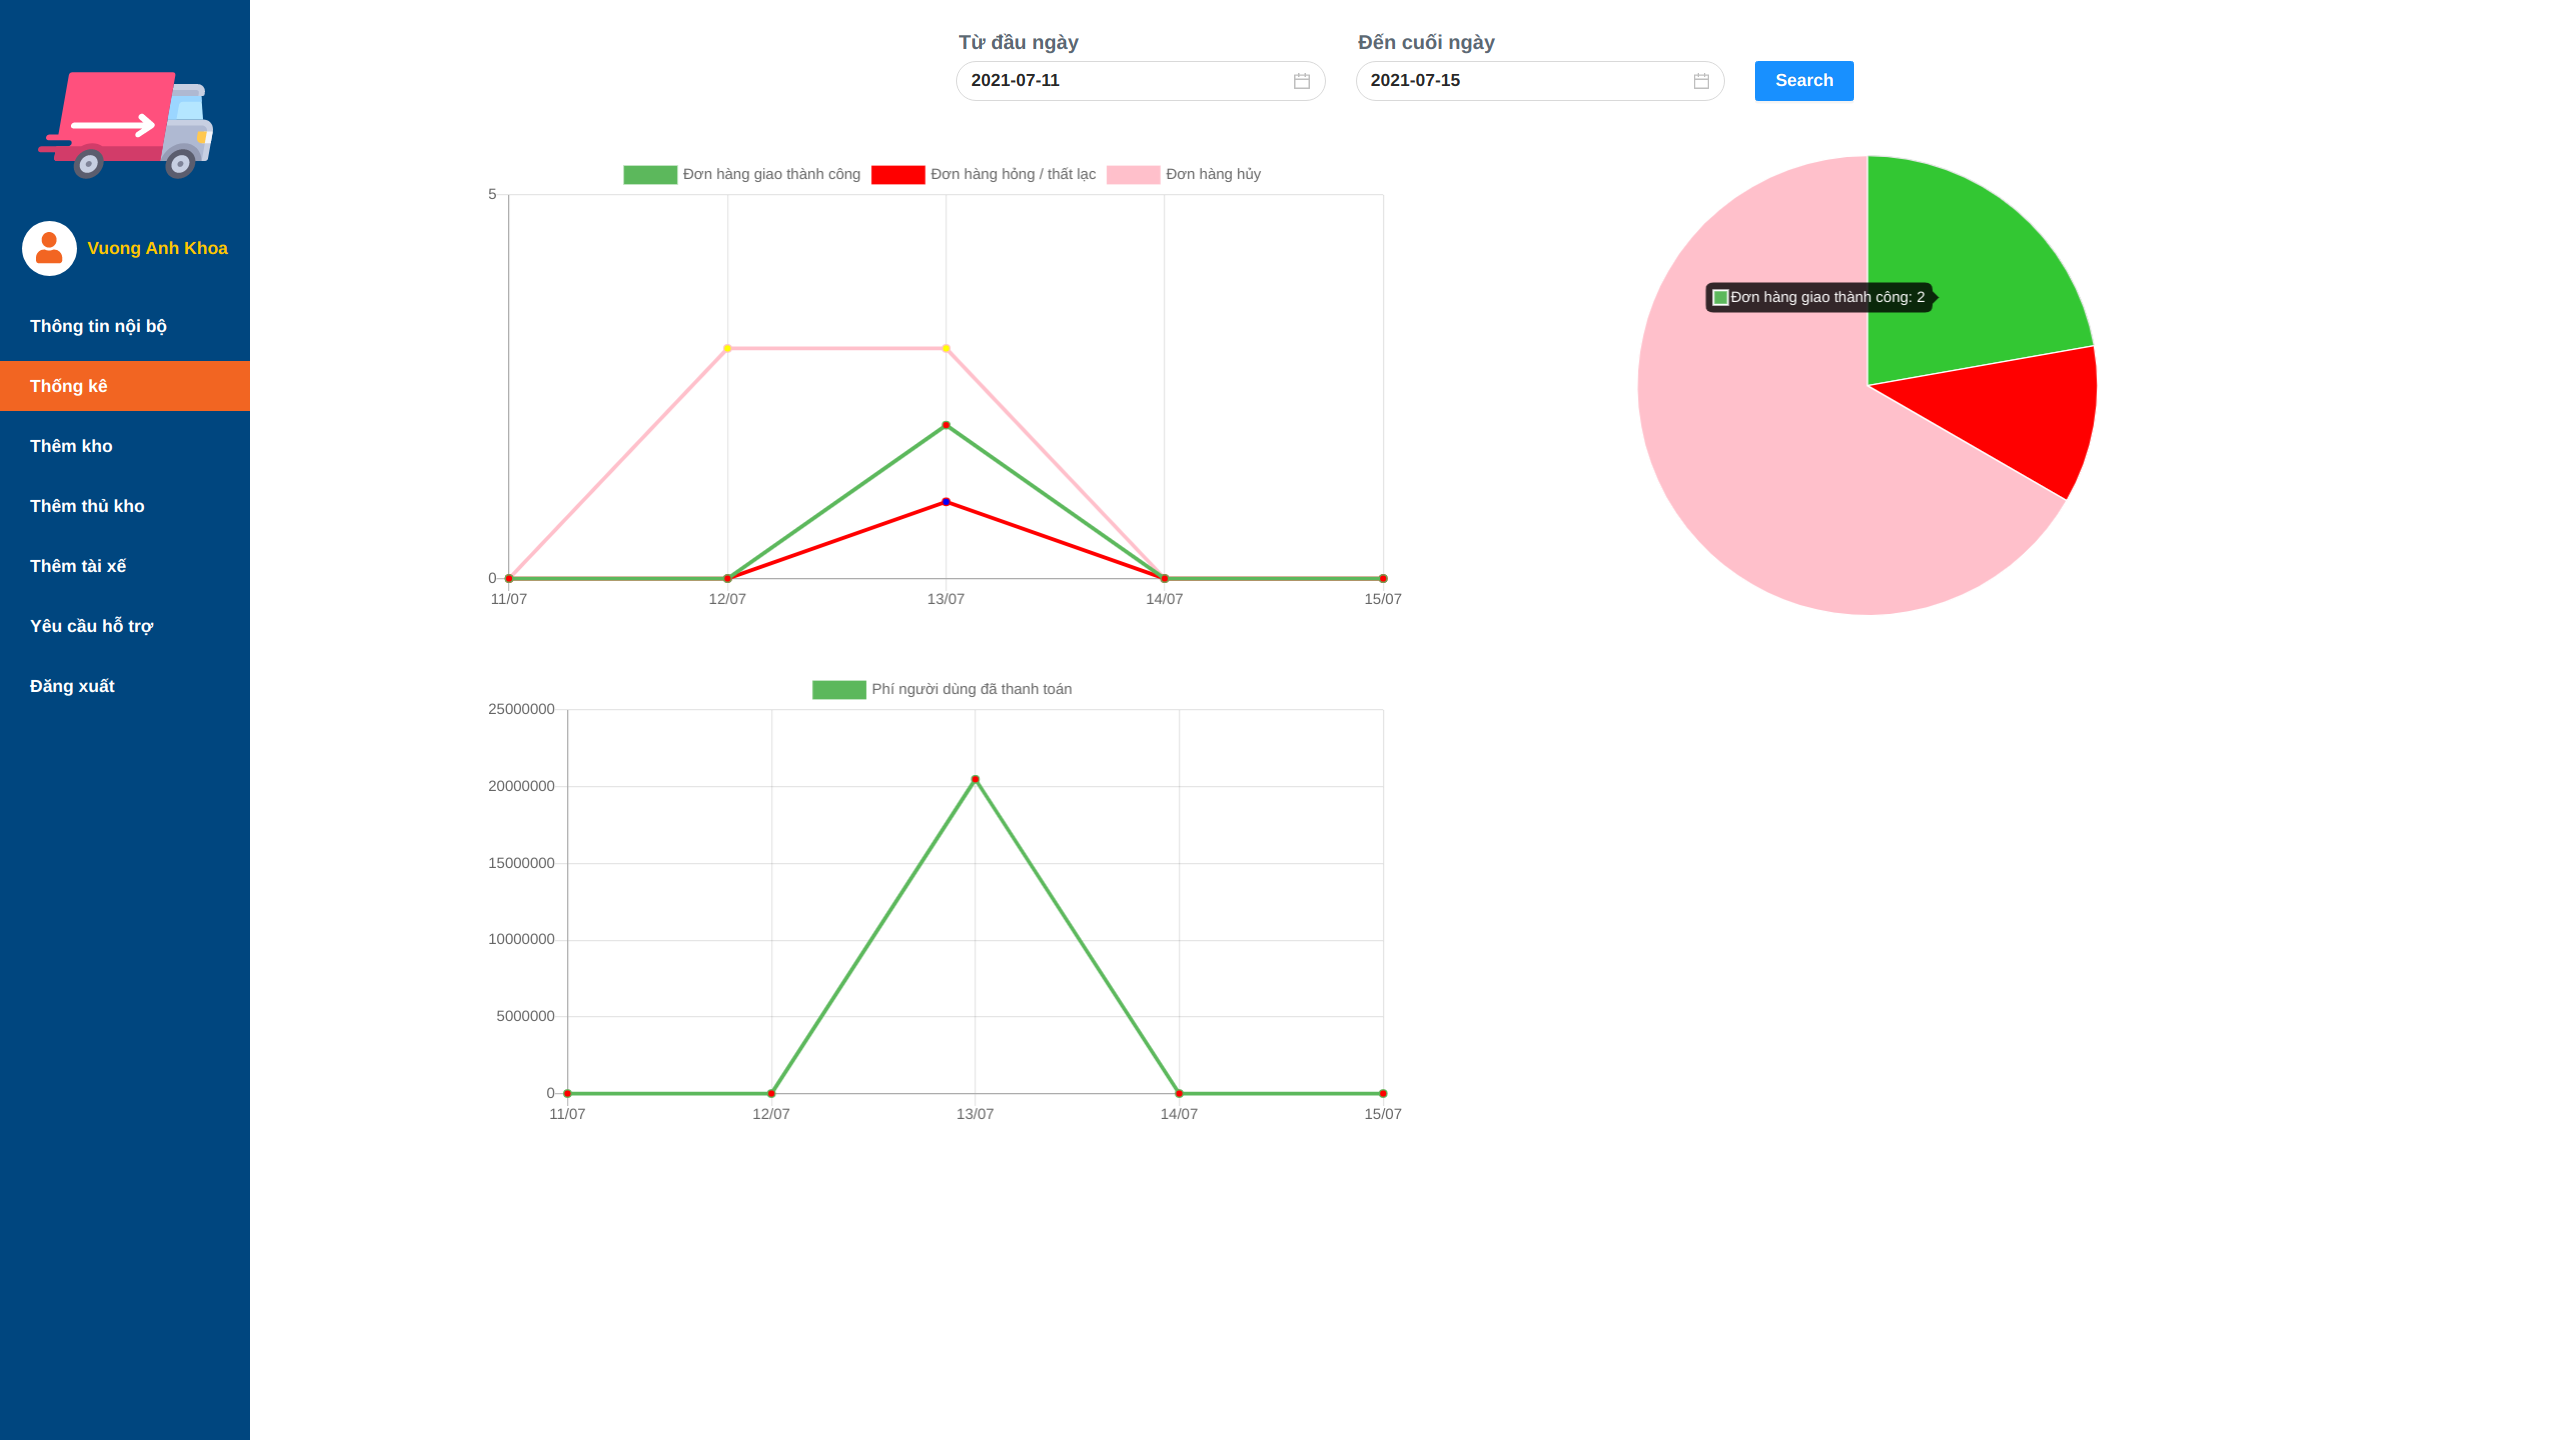
\includegraphics[width=1\textwidth]{/admin/admin_statistic.png}
		\centering
		\caption{Xem thống kê đơn hàng và số tiền khách hàng đã thanh toán}
	\end{figure}

	\item \textbf{Thêm tài xế vào hệ thống}
	\begin{figure}[H]
		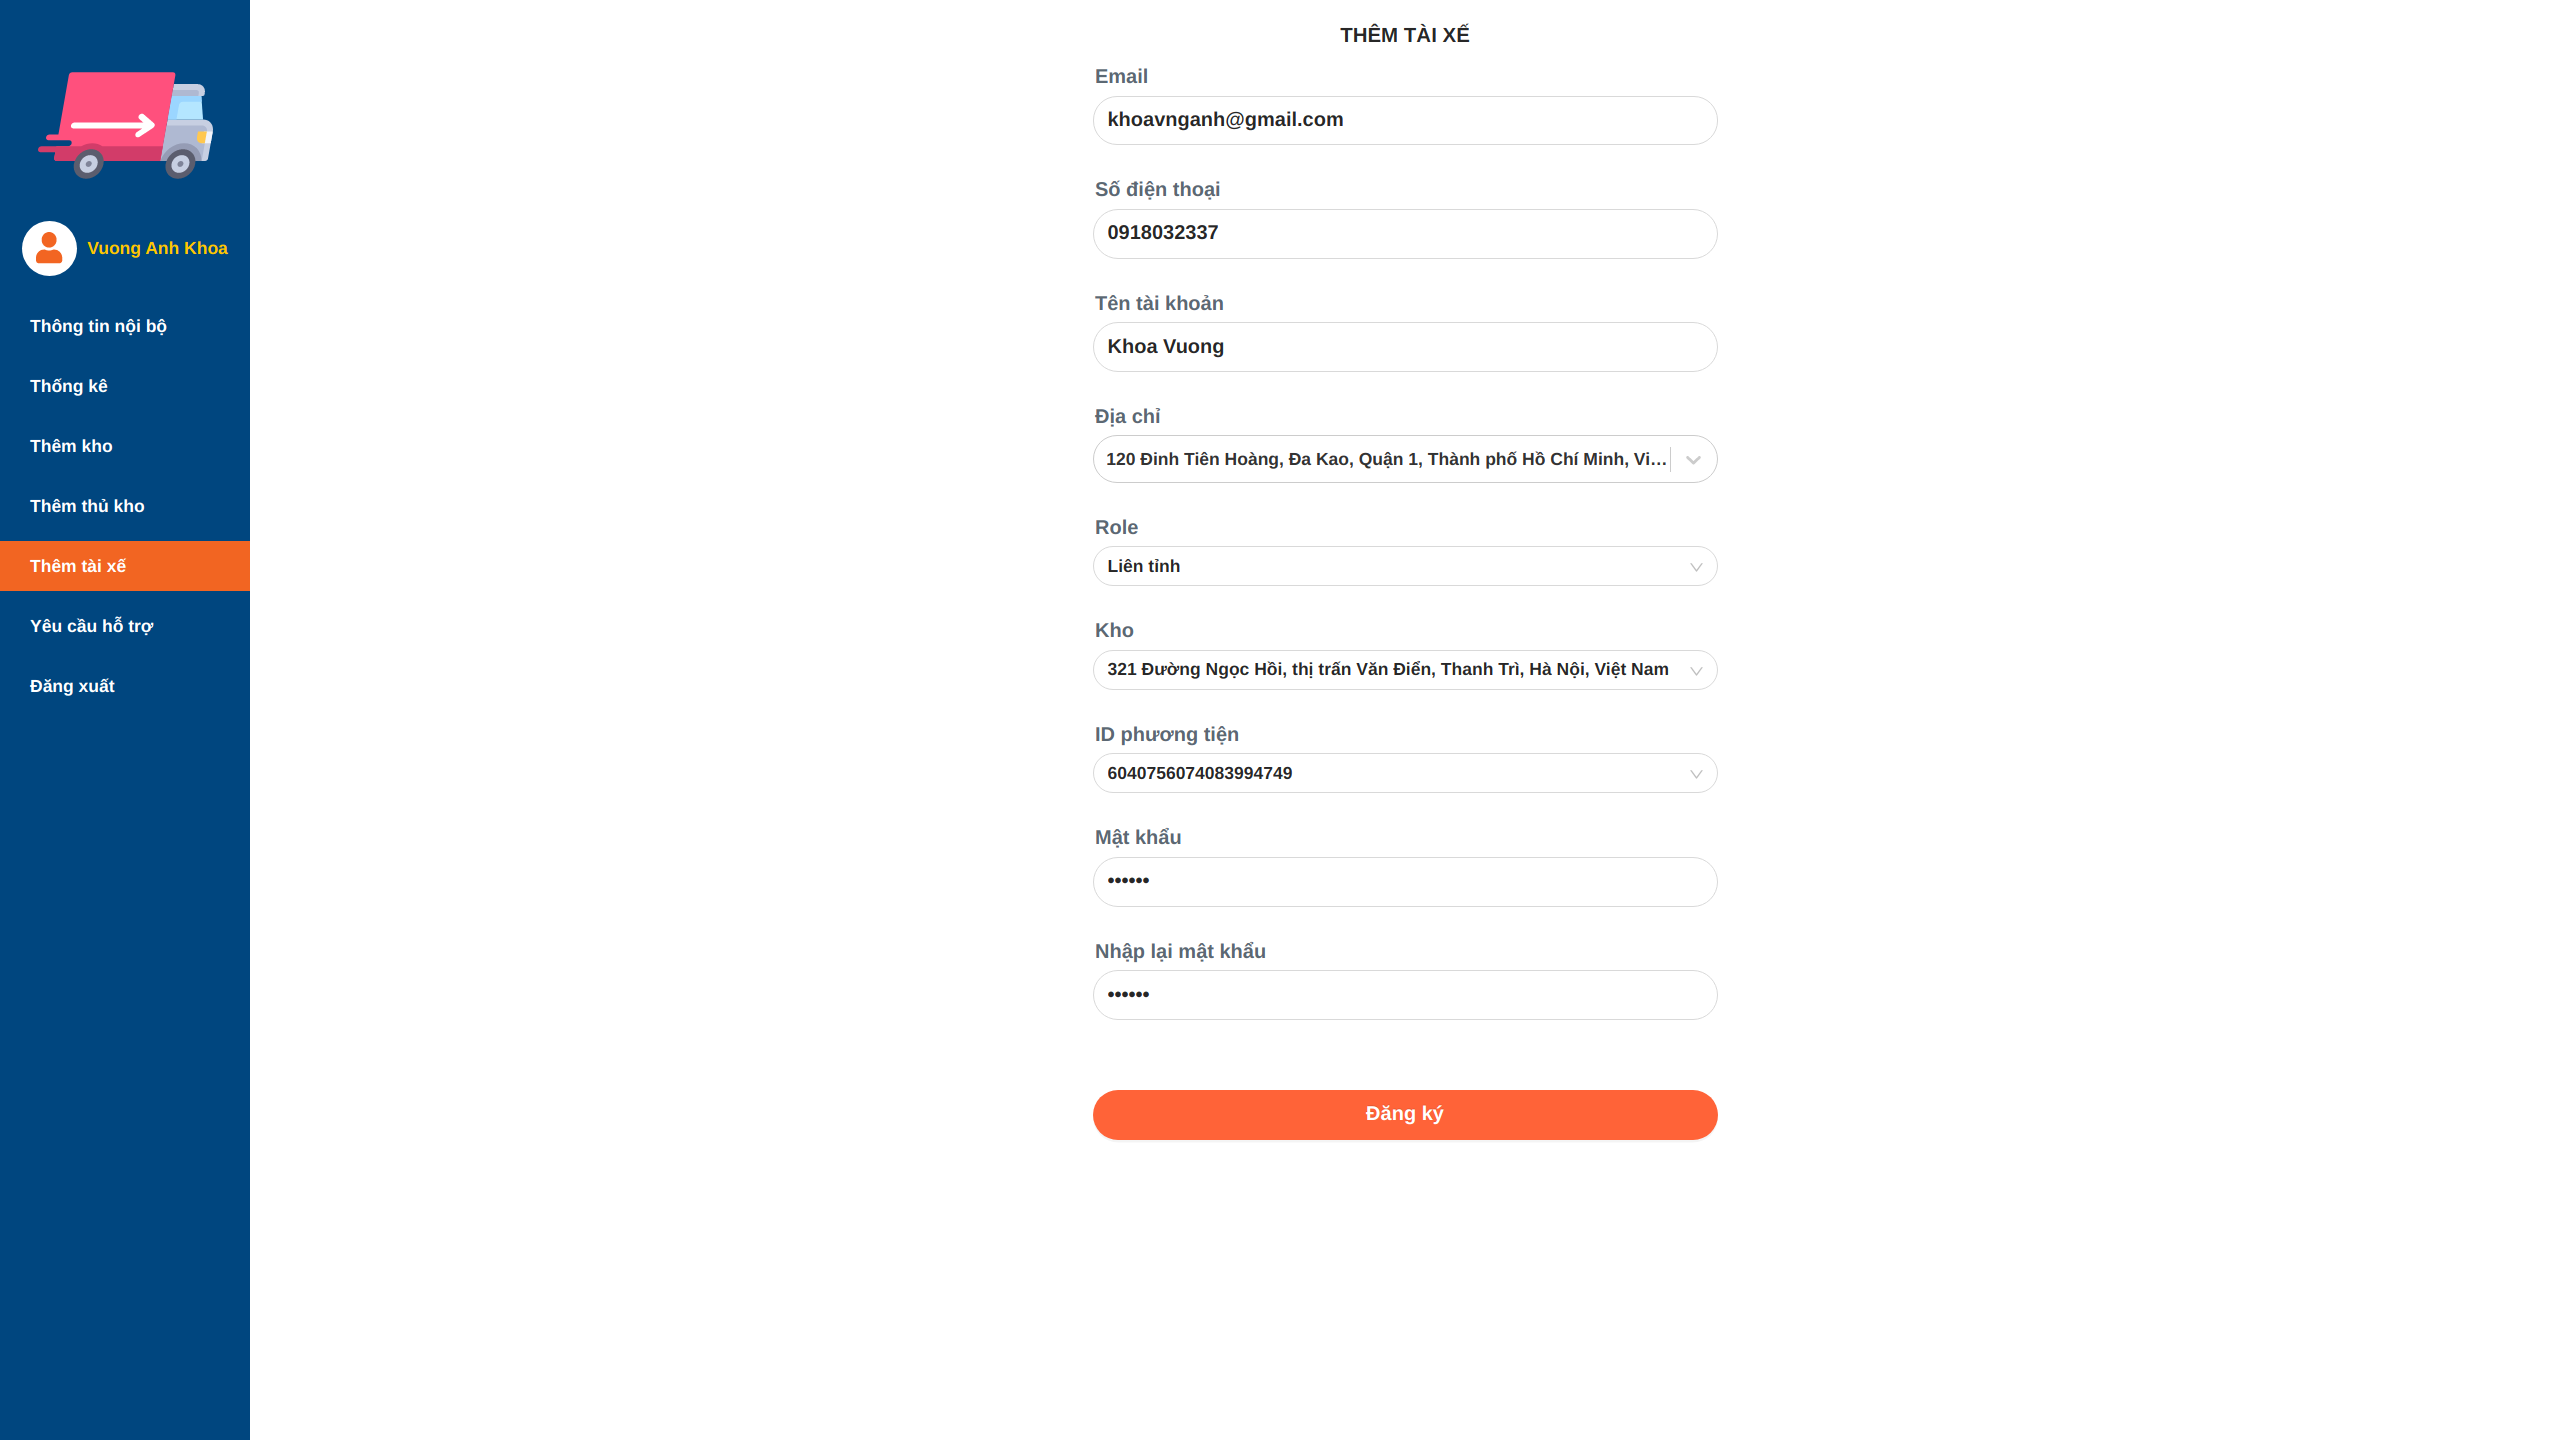
\includegraphics[width=1\textwidth]{/admin/admin_add_driver.png}
		\centering
		\caption{Thêm tài xế vào hệ thống}
	\end{figure}


	\item \textbf{Thêm thủ kho vào hệ thống}
	\begin{figure}[H]
		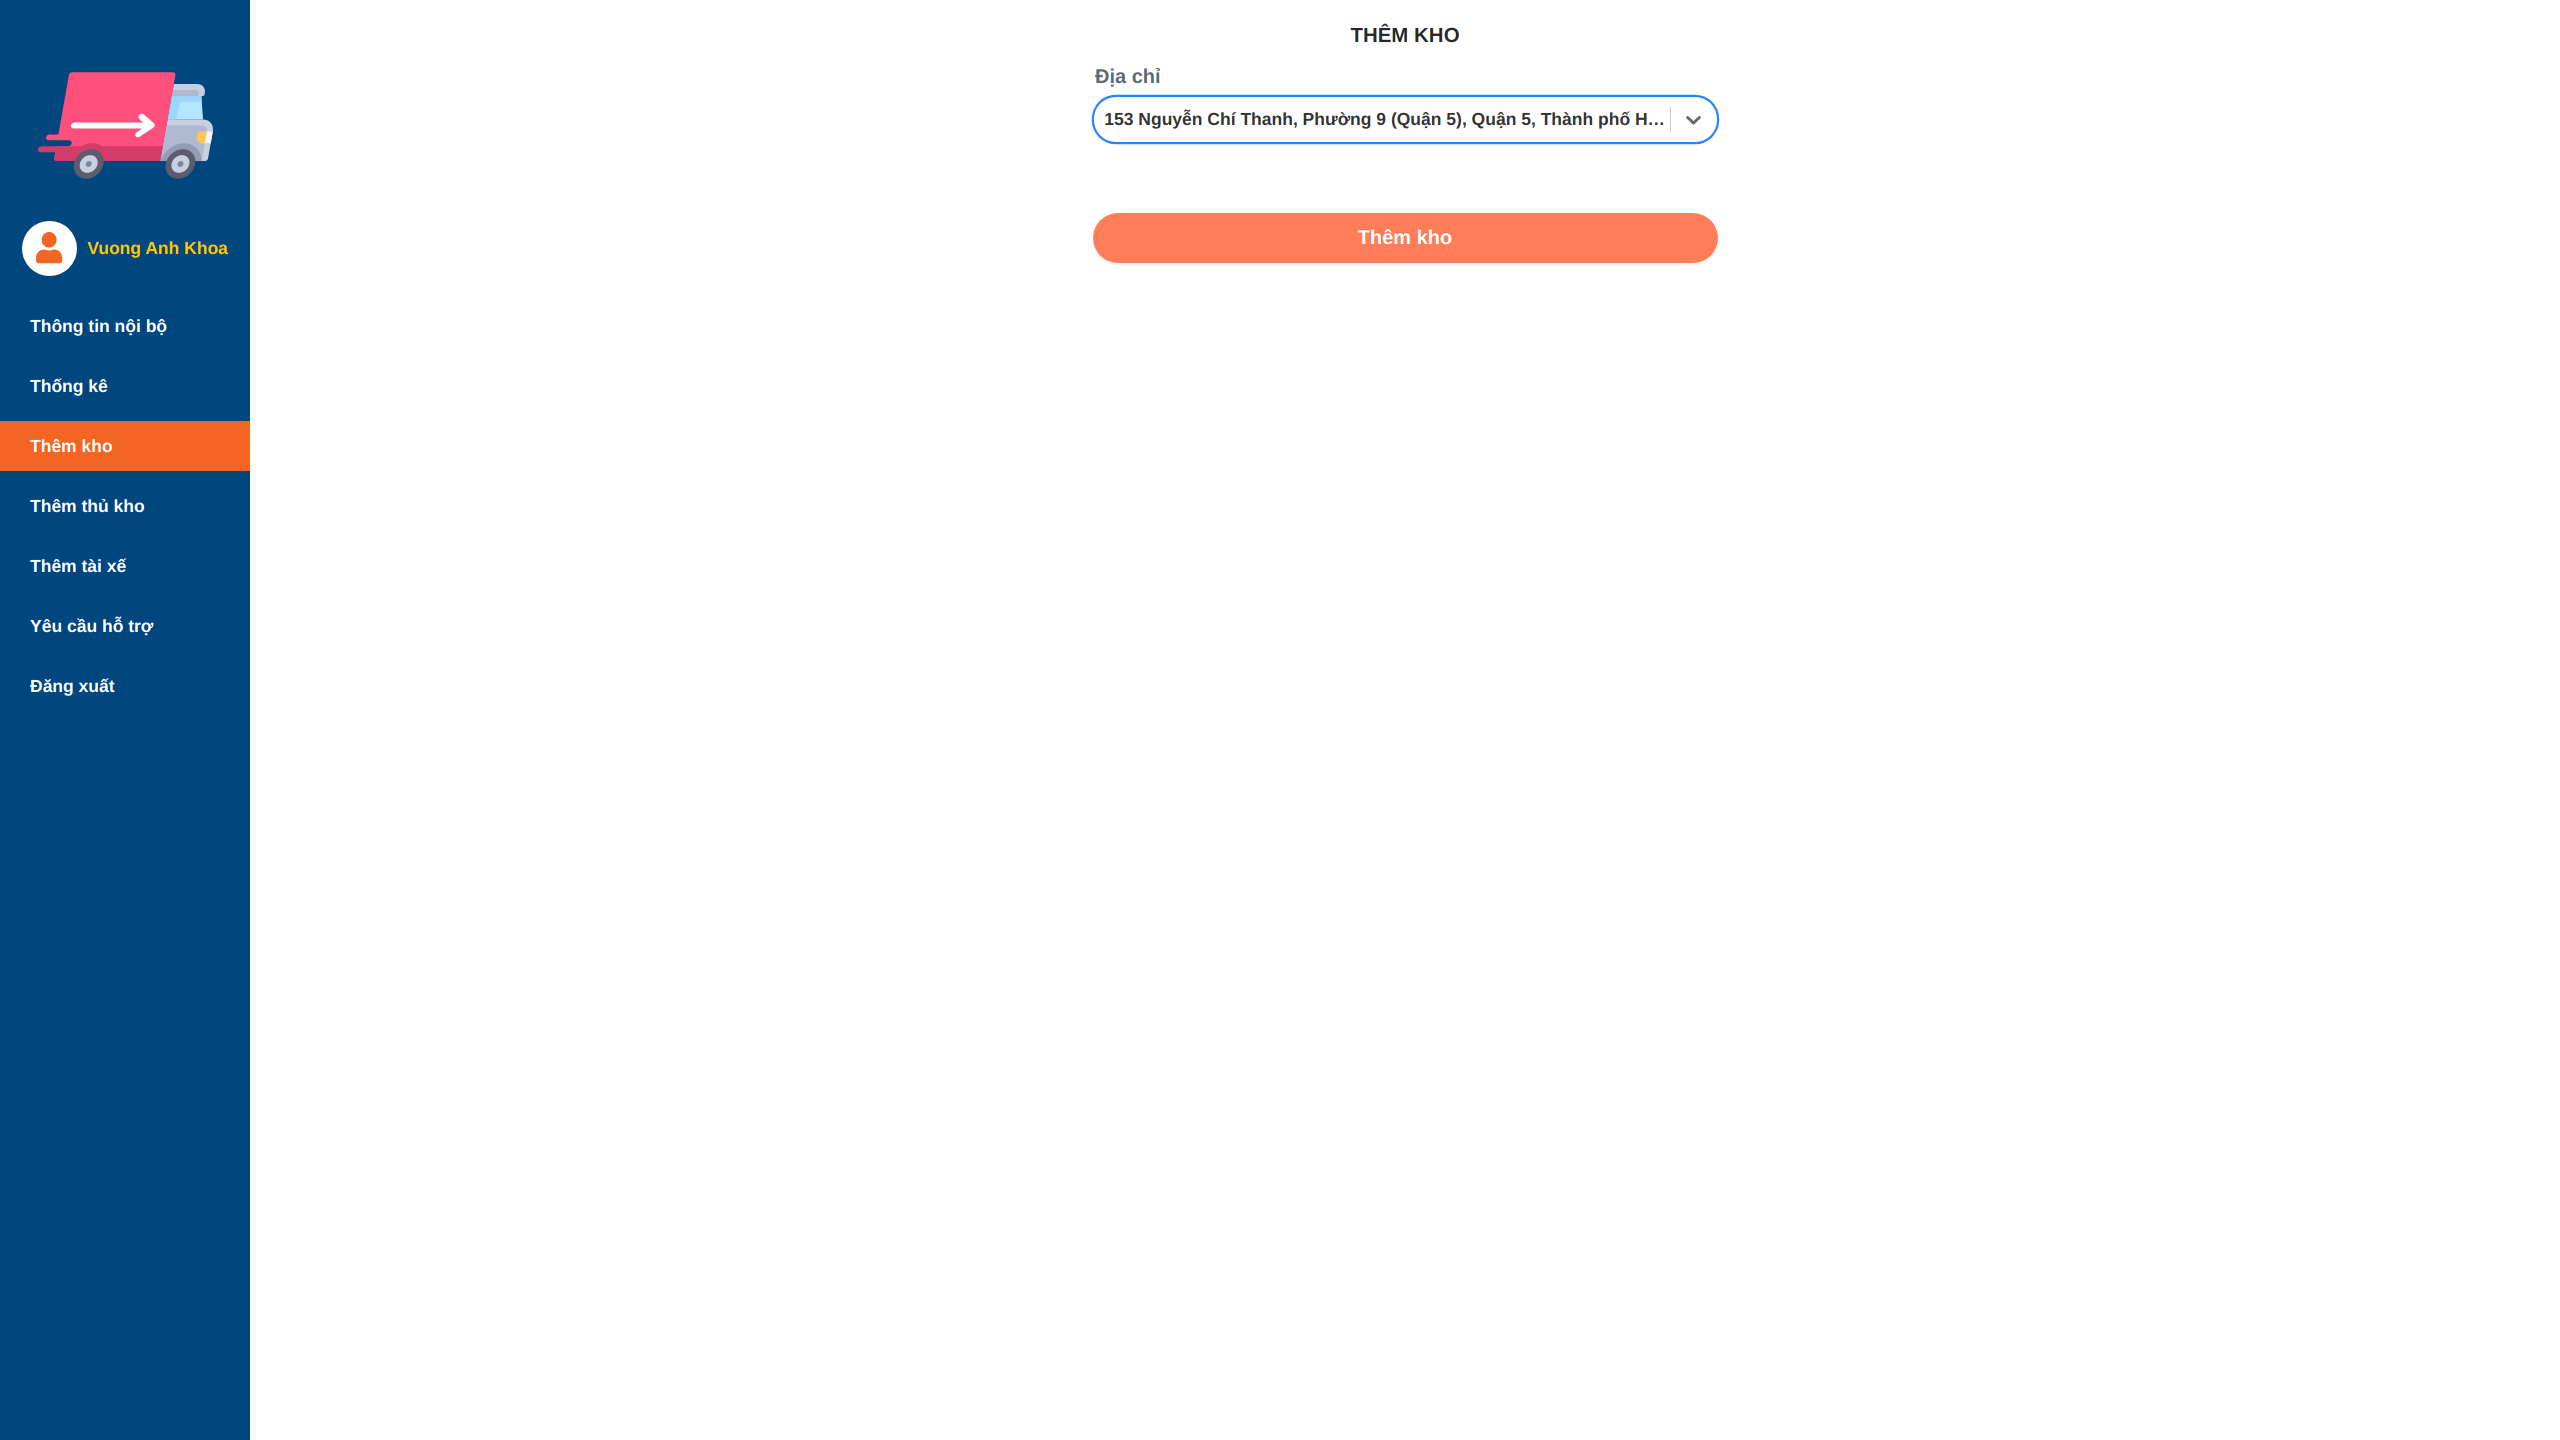
\includegraphics[width=1\textwidth]{/admin/admin_add_stock.png}
		\centering
		\caption{Thêm kho vào hệ thống}
	\end{figure}
	
	\begin{figure}[H]
		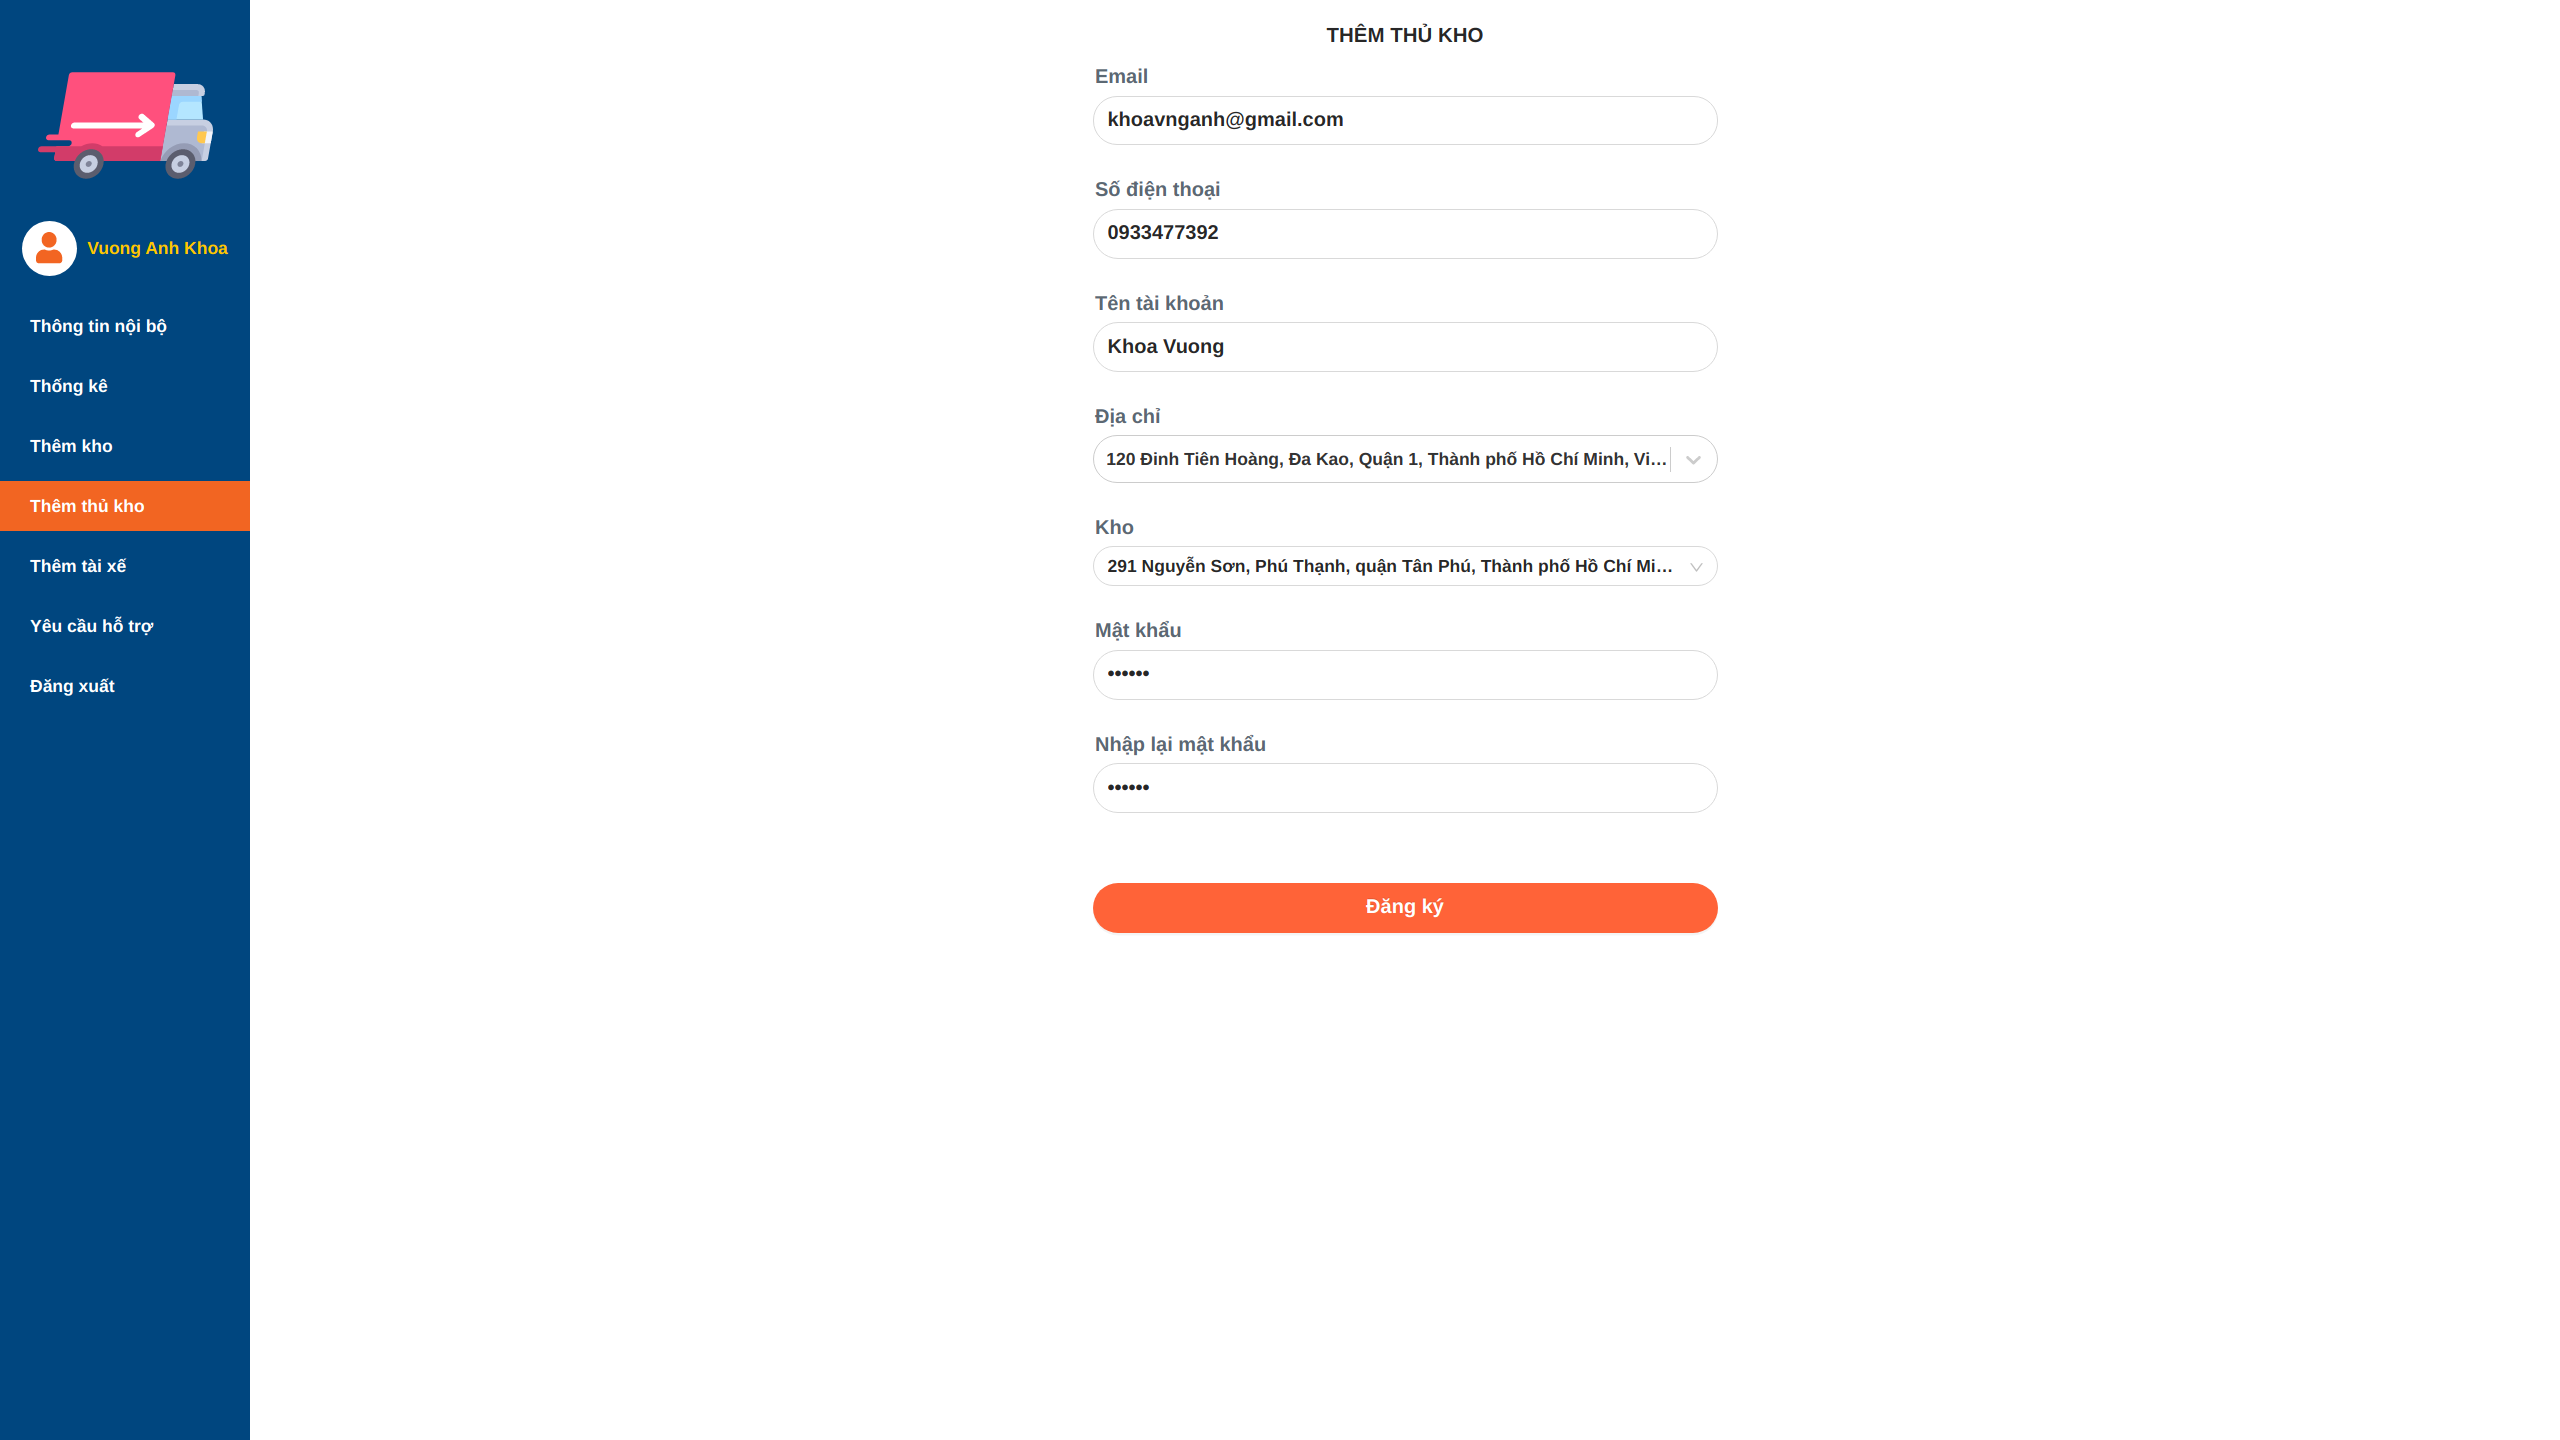
\includegraphics[width=1\textwidth]{/admin/admin_add_stock_keeper.png}
		\centering
		\caption{Thêm thủ kho vào hệ thống}
	\end{figure}

	\item \textbf{Xem yêu cầu hỗ trợ}
	\begin{figure}[H]
		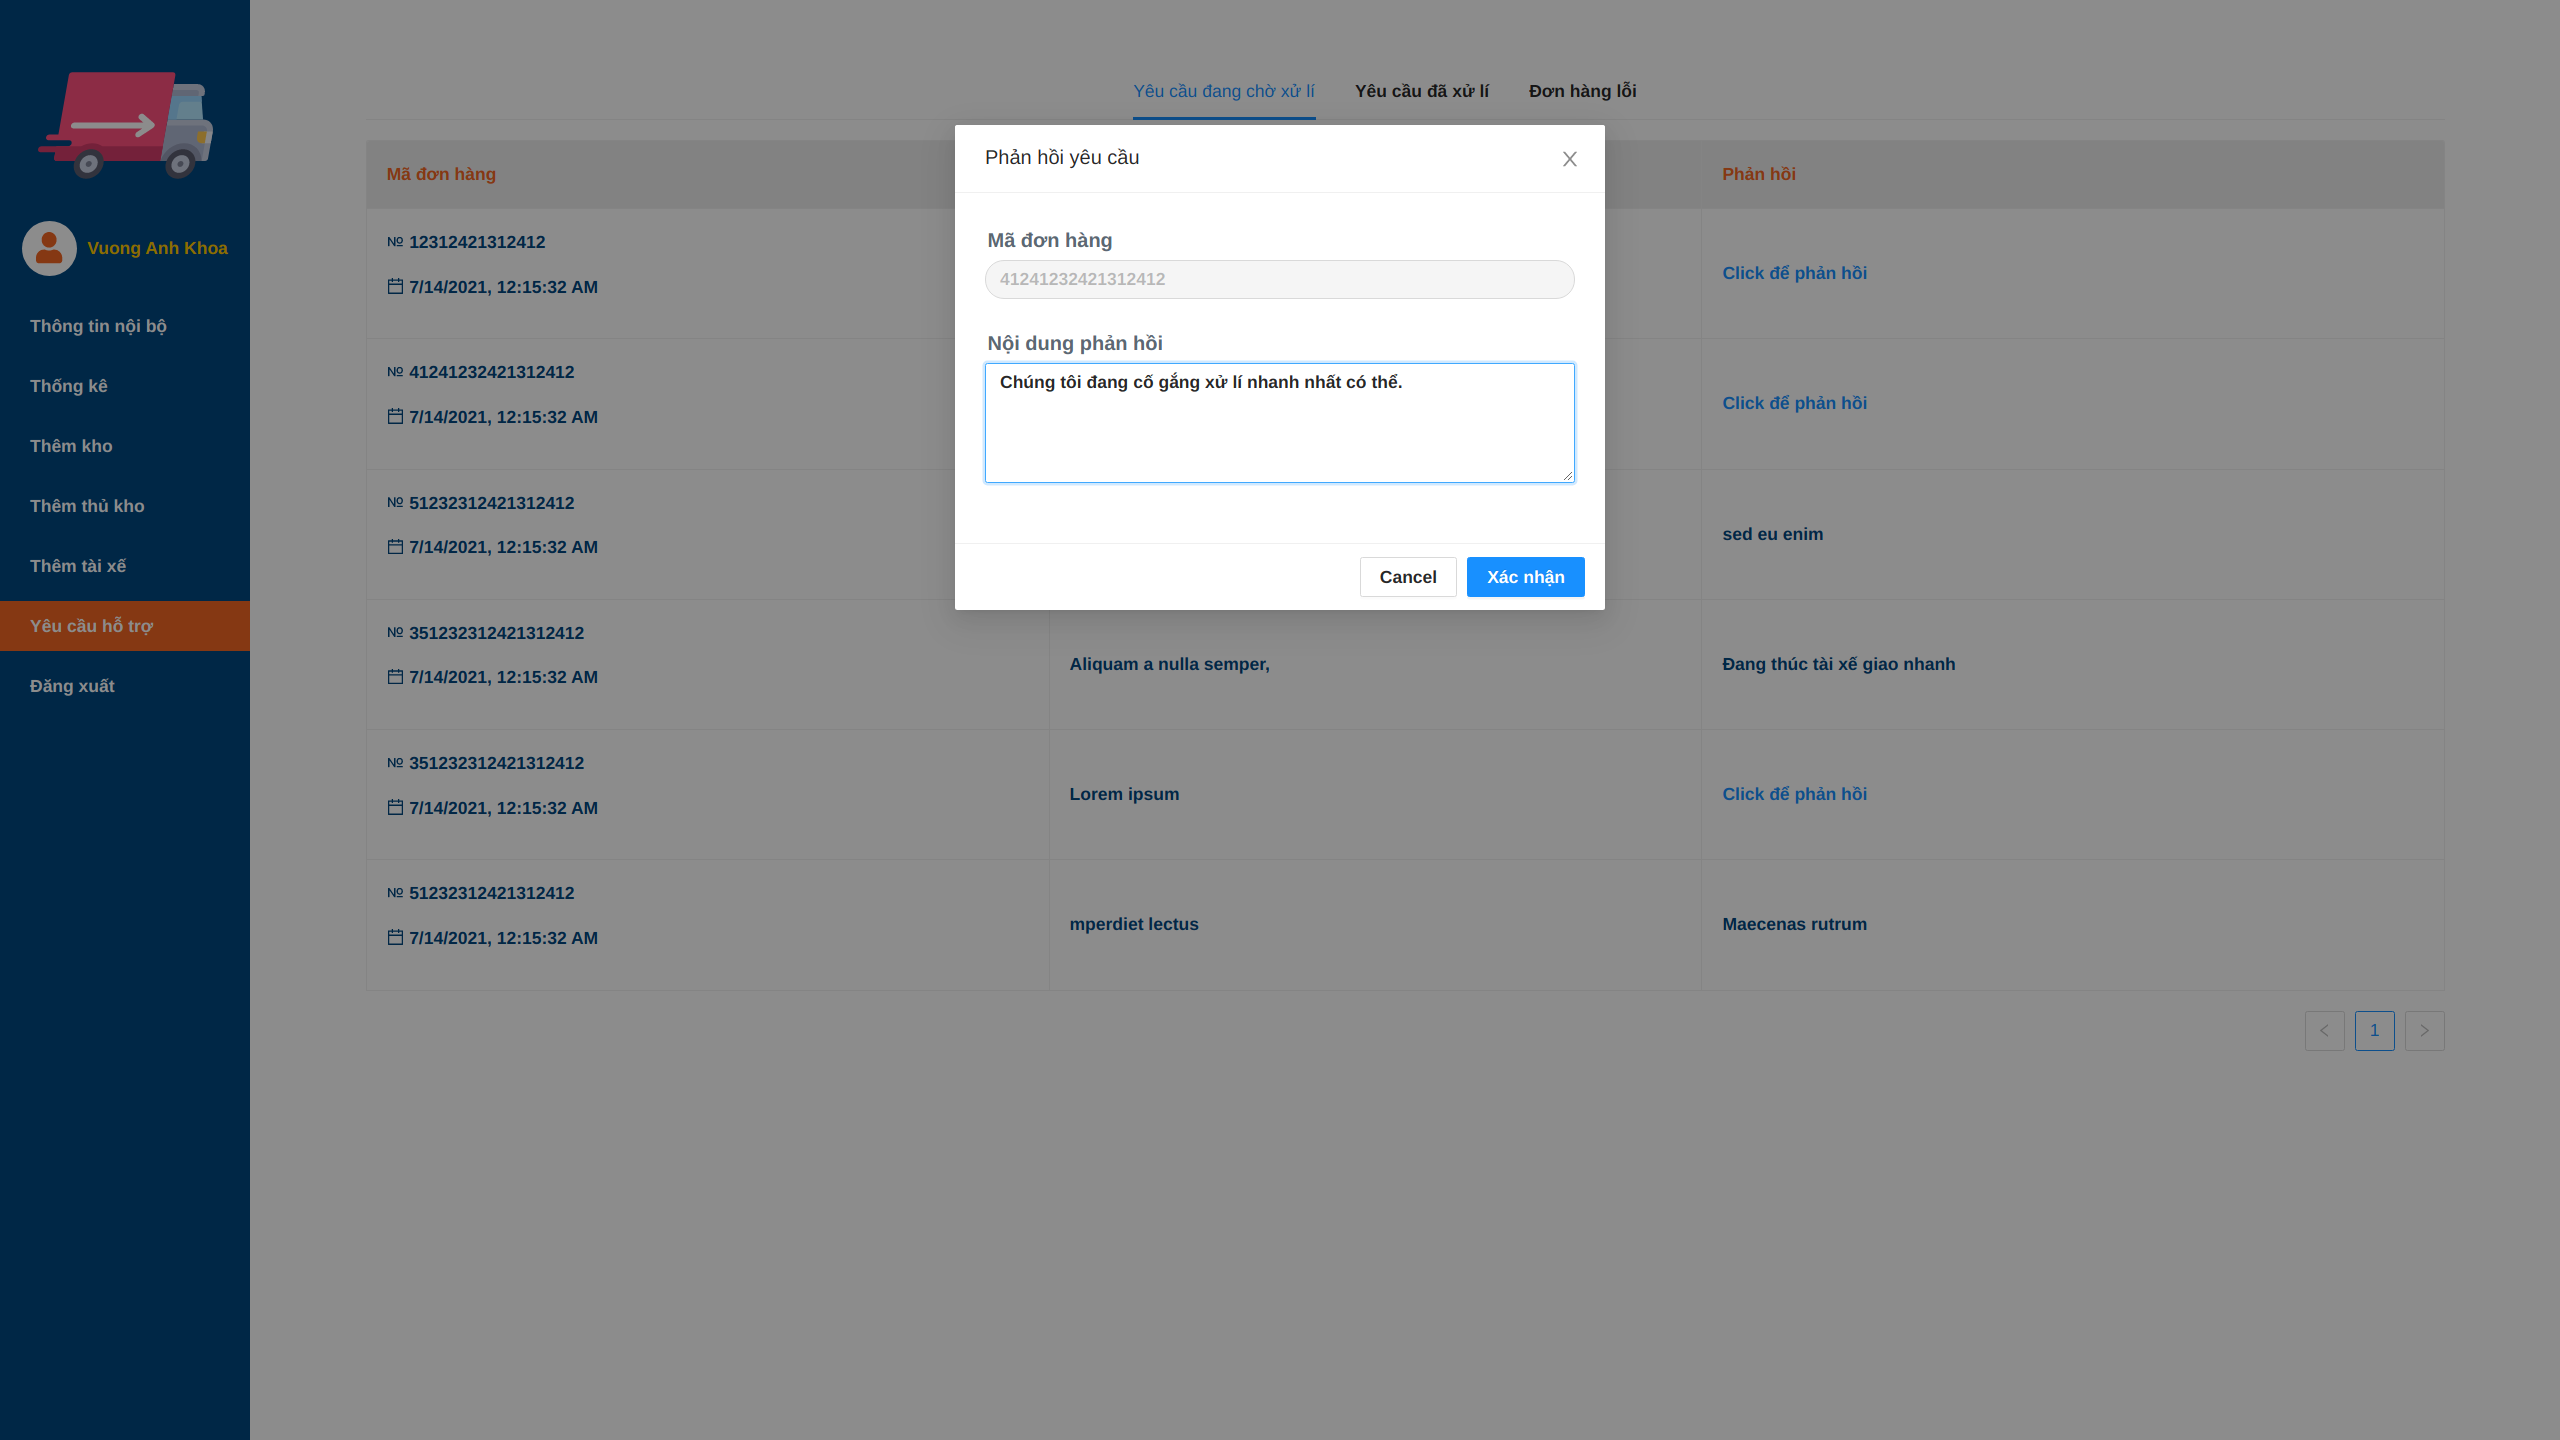
\includegraphics[width=1\textwidth]{/admin/admin_requests_reply.png}
		\centering
		\caption{Giao diện trả lời những yêu cần cầu hỗ trợ từ khách hàng}
	\end{figure}
	
	\begin{figure}[H]
		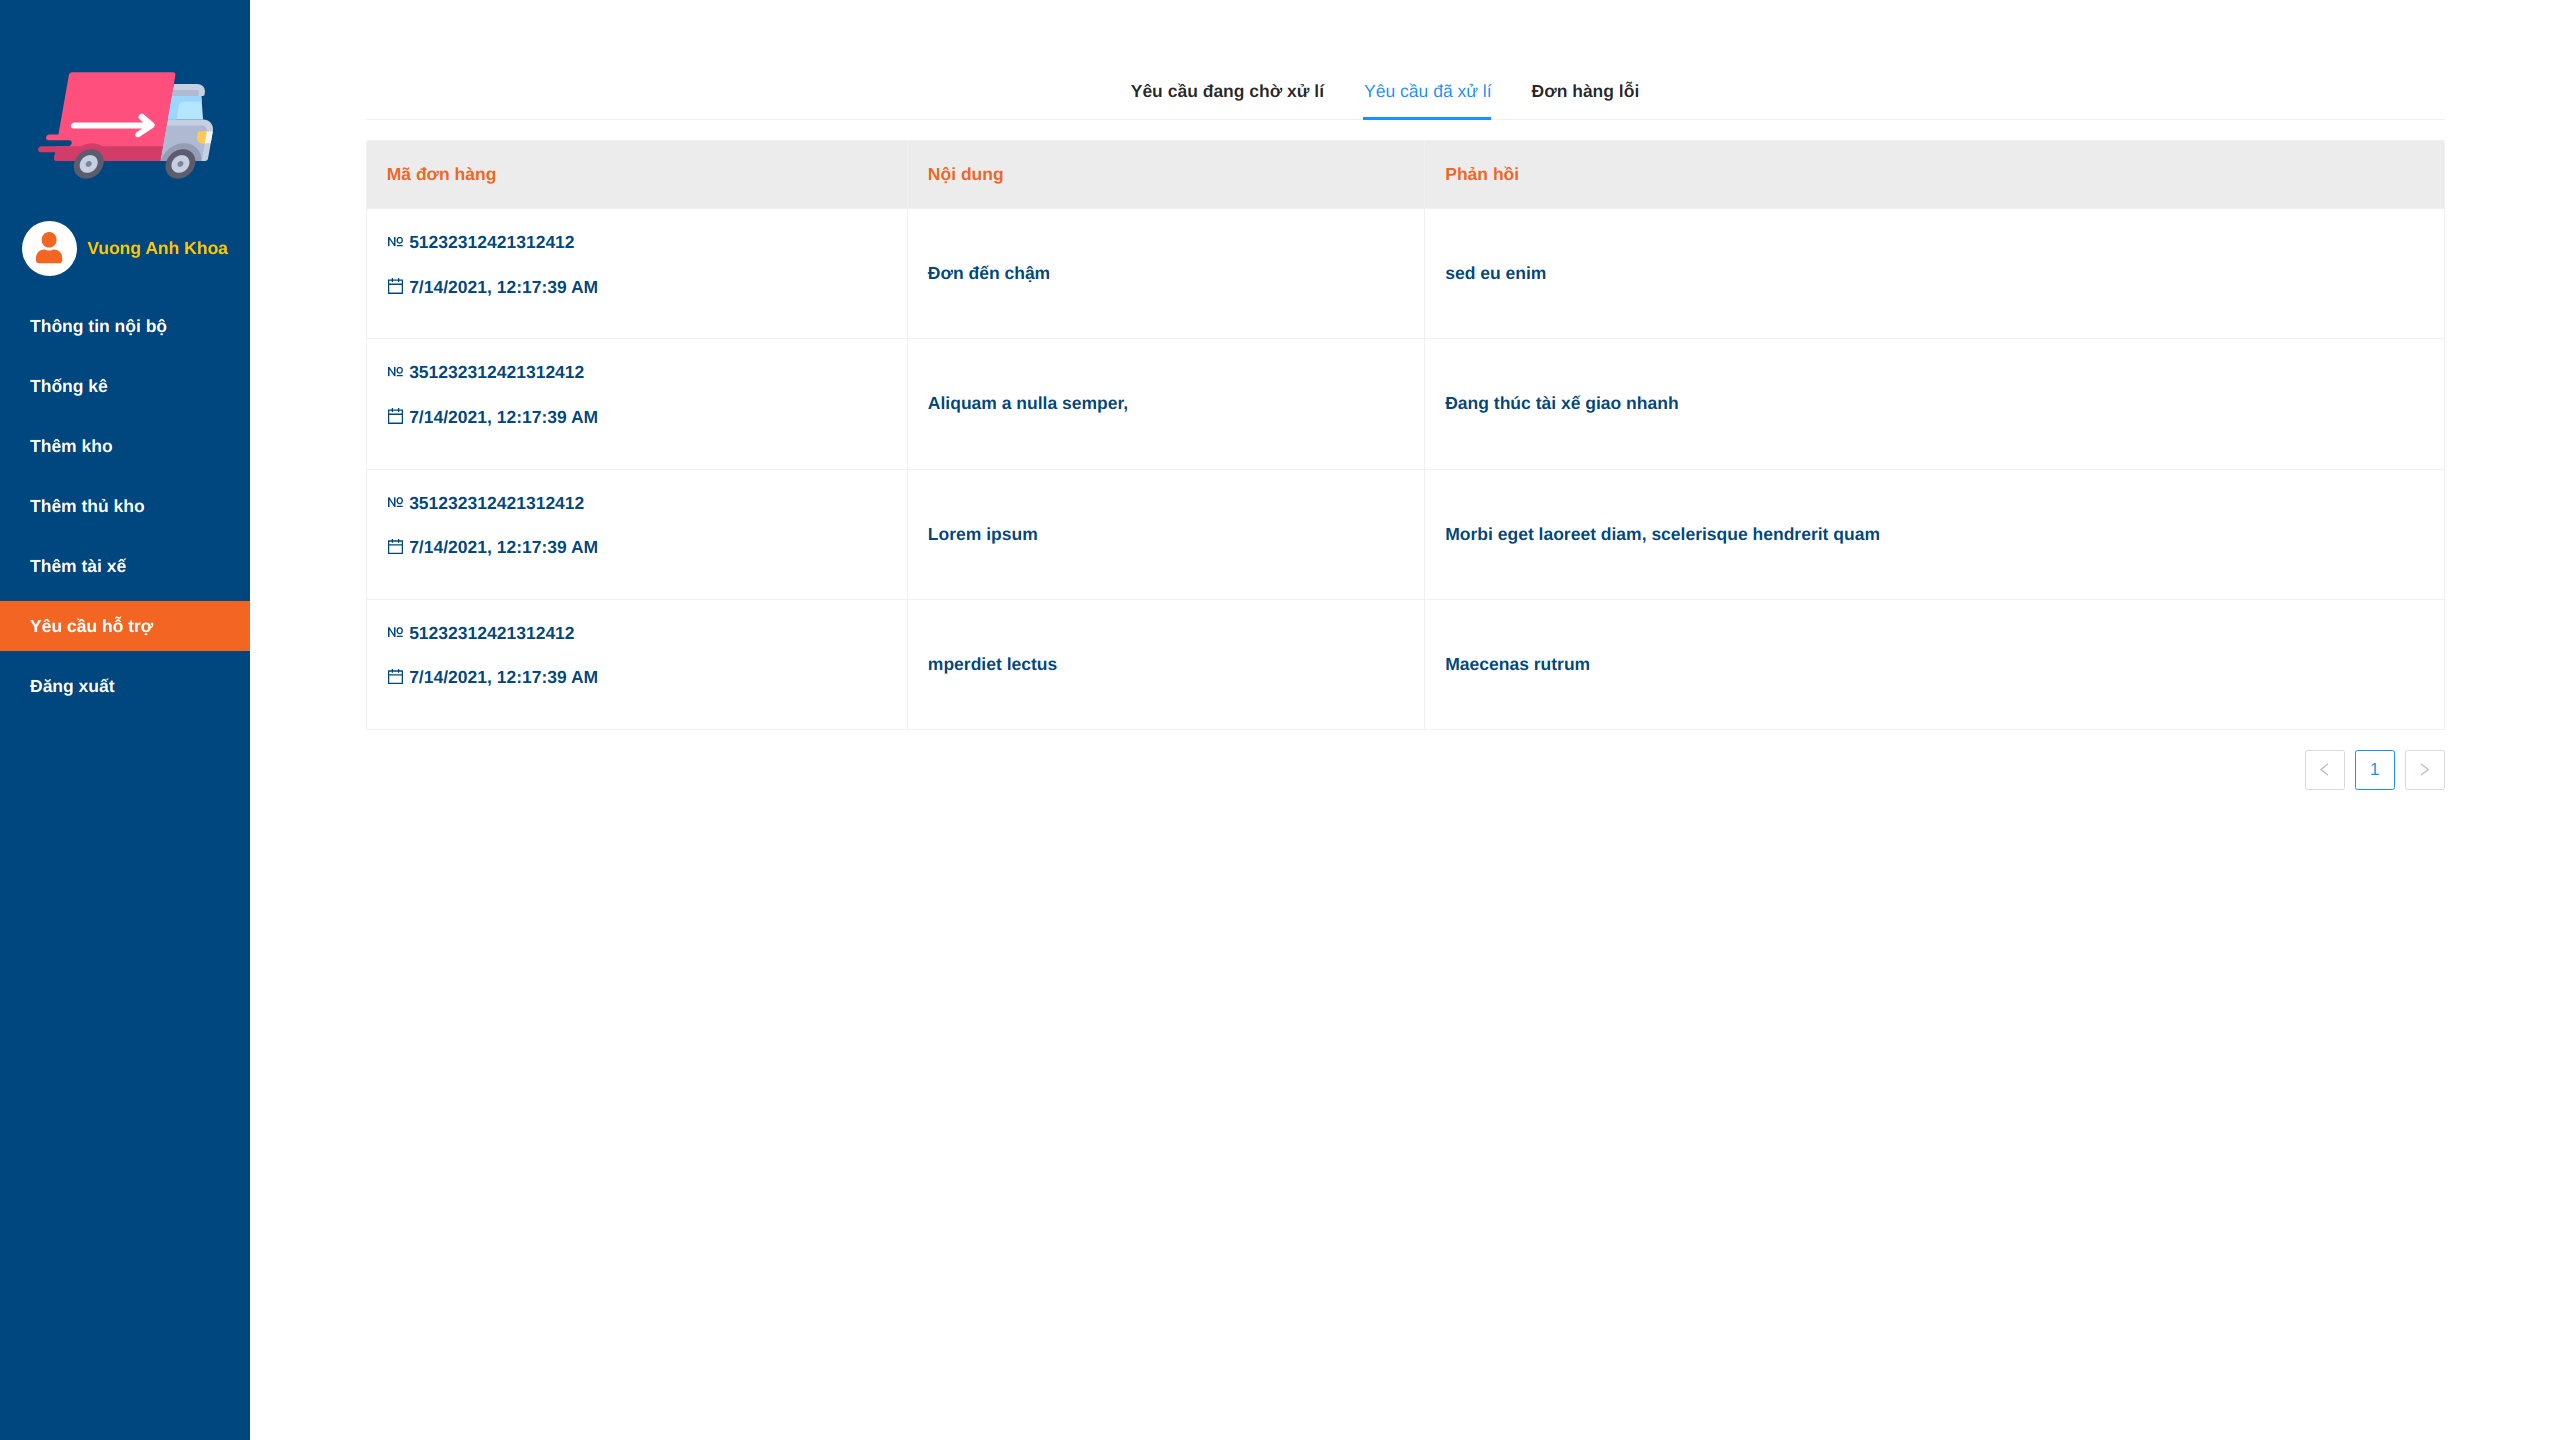
\includegraphics[width=1\textwidth]{/admin/admin_requests_done.png}
		\centering
		\caption{Giao diện xem lại những yêu cầu hỗ trợ đã trả lời}
	\end{figure}

	\item \textbf{Xem báo cáo sự cố}
	\begin{figure}[H]
		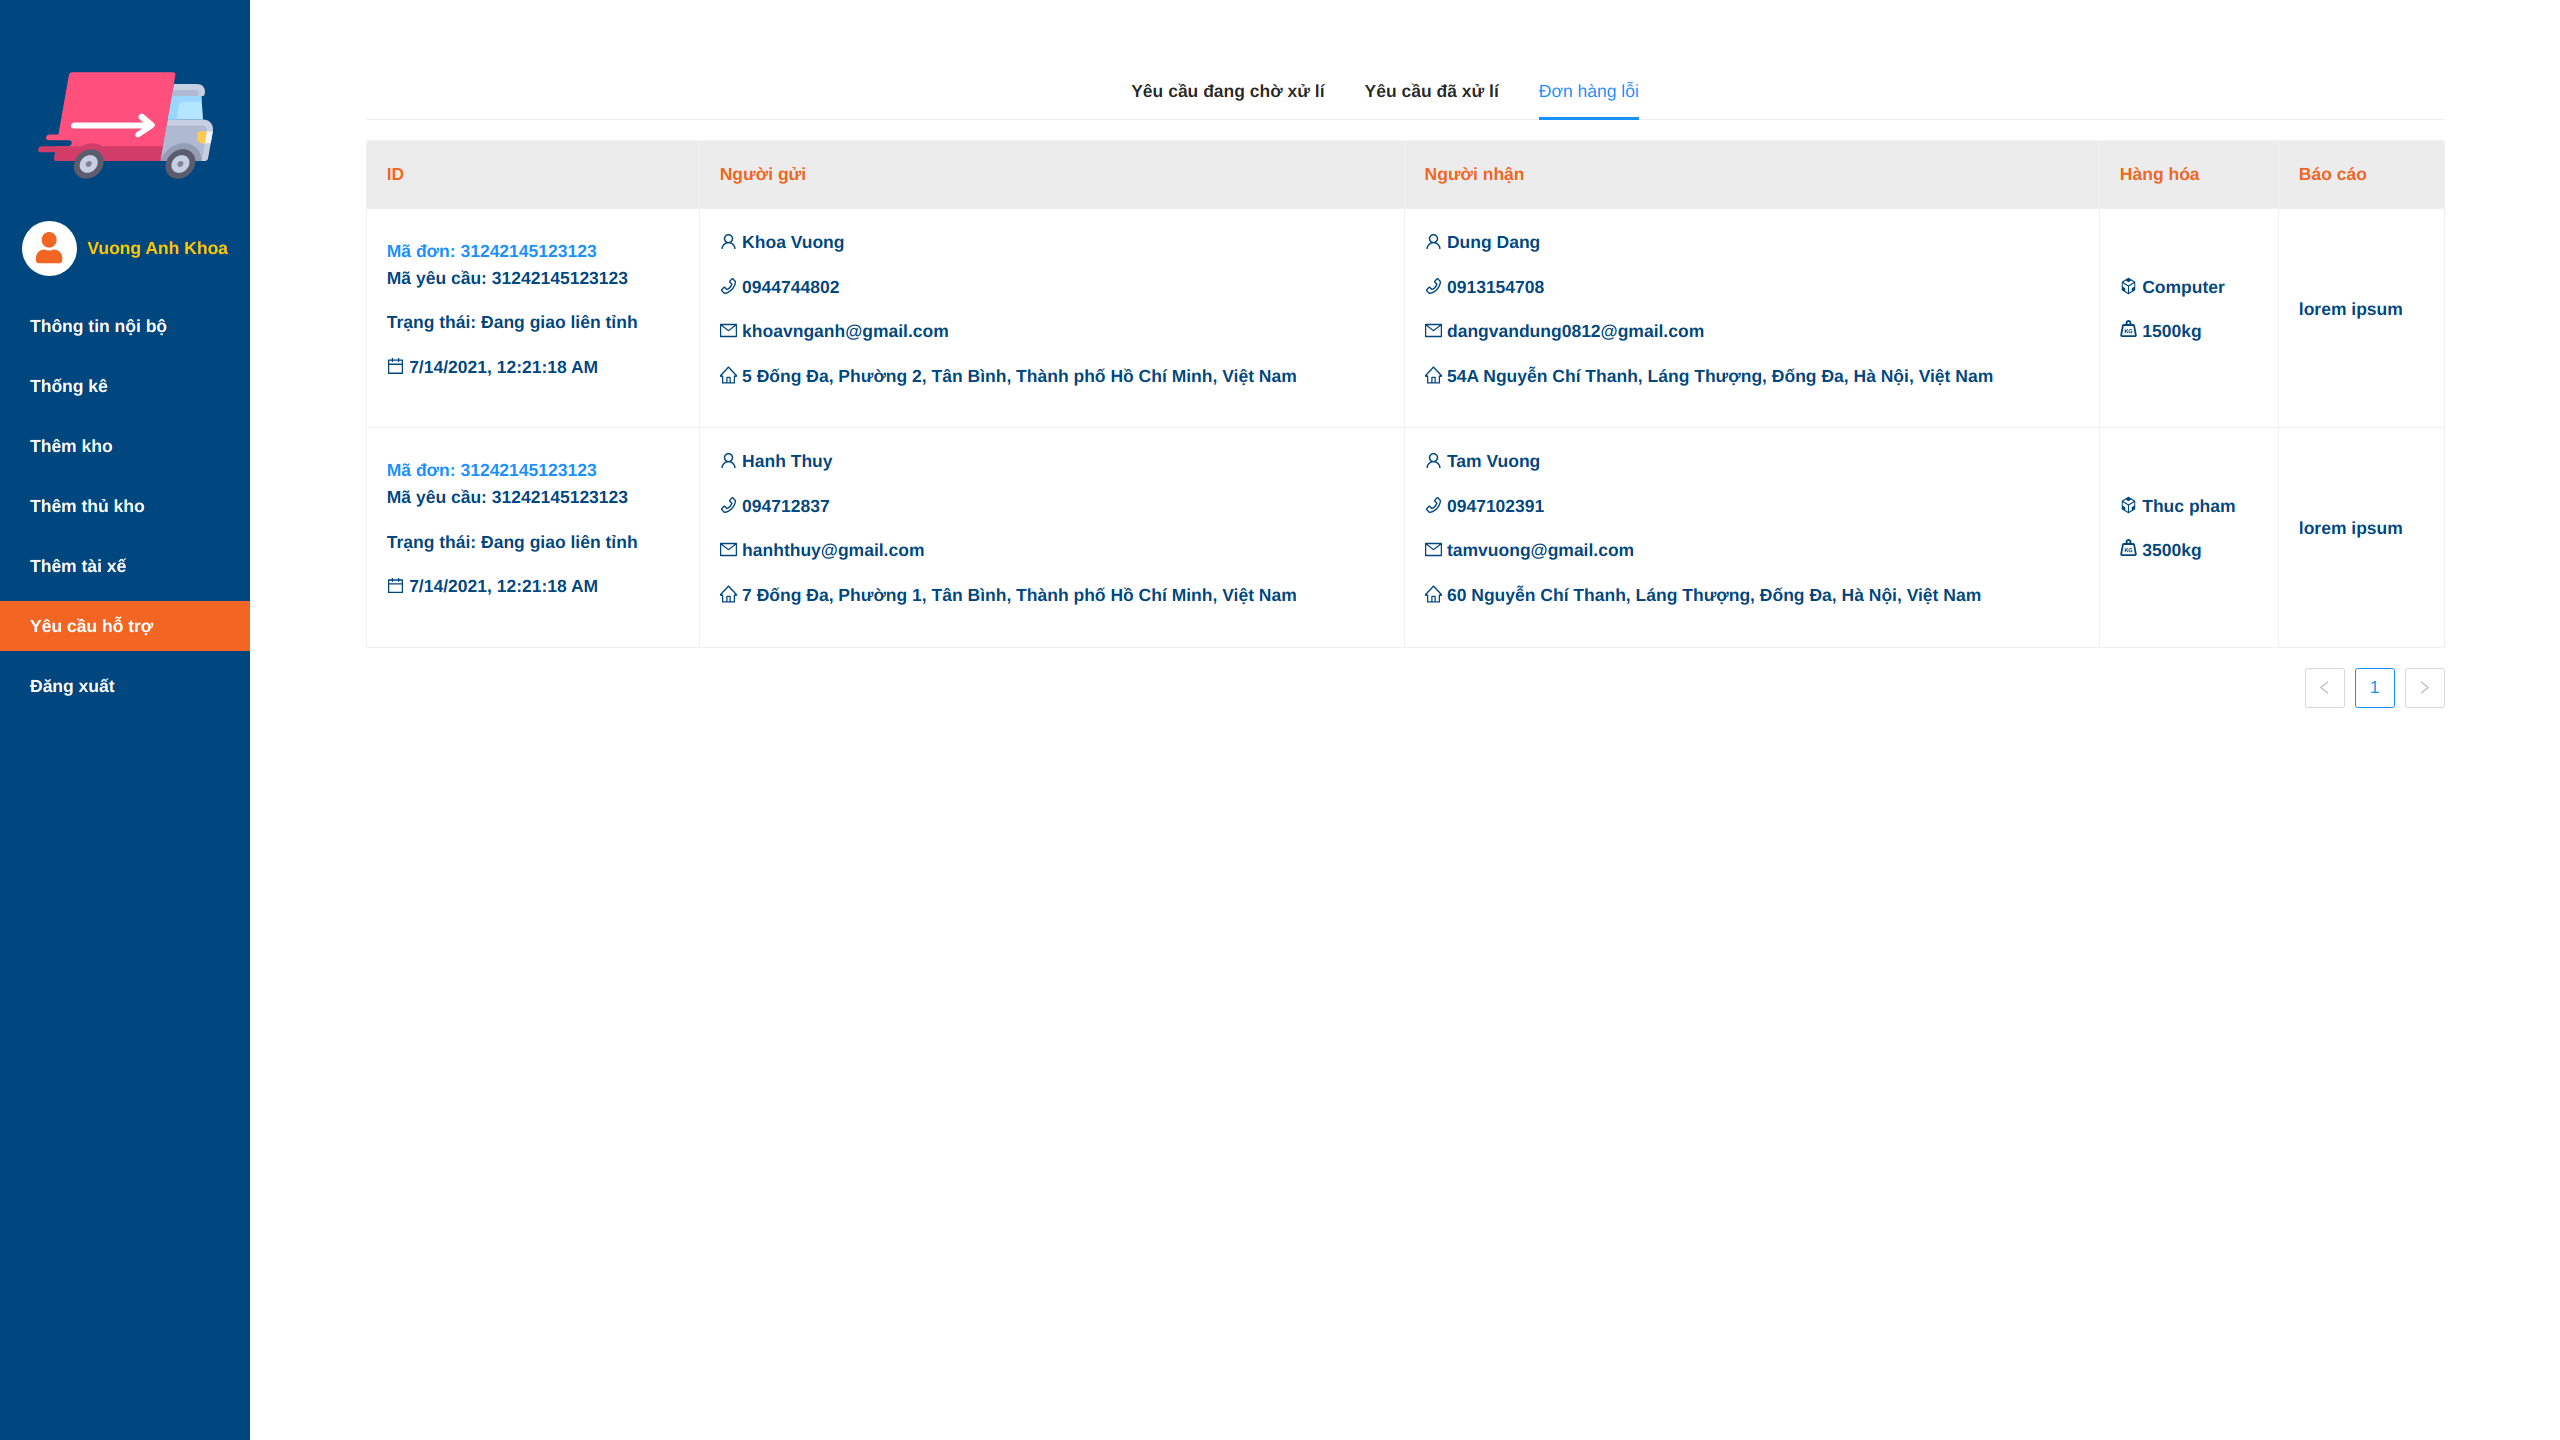
\includegraphics[width=1\textwidth]{/admin/admin_issues.png}
		\centering
		\caption{Giao diện xem những sự cố báo cáo từ tài xế}
	\end{figure}


	\item \textbf{Xử lý sự cố}
	\begin{figure}[H]
		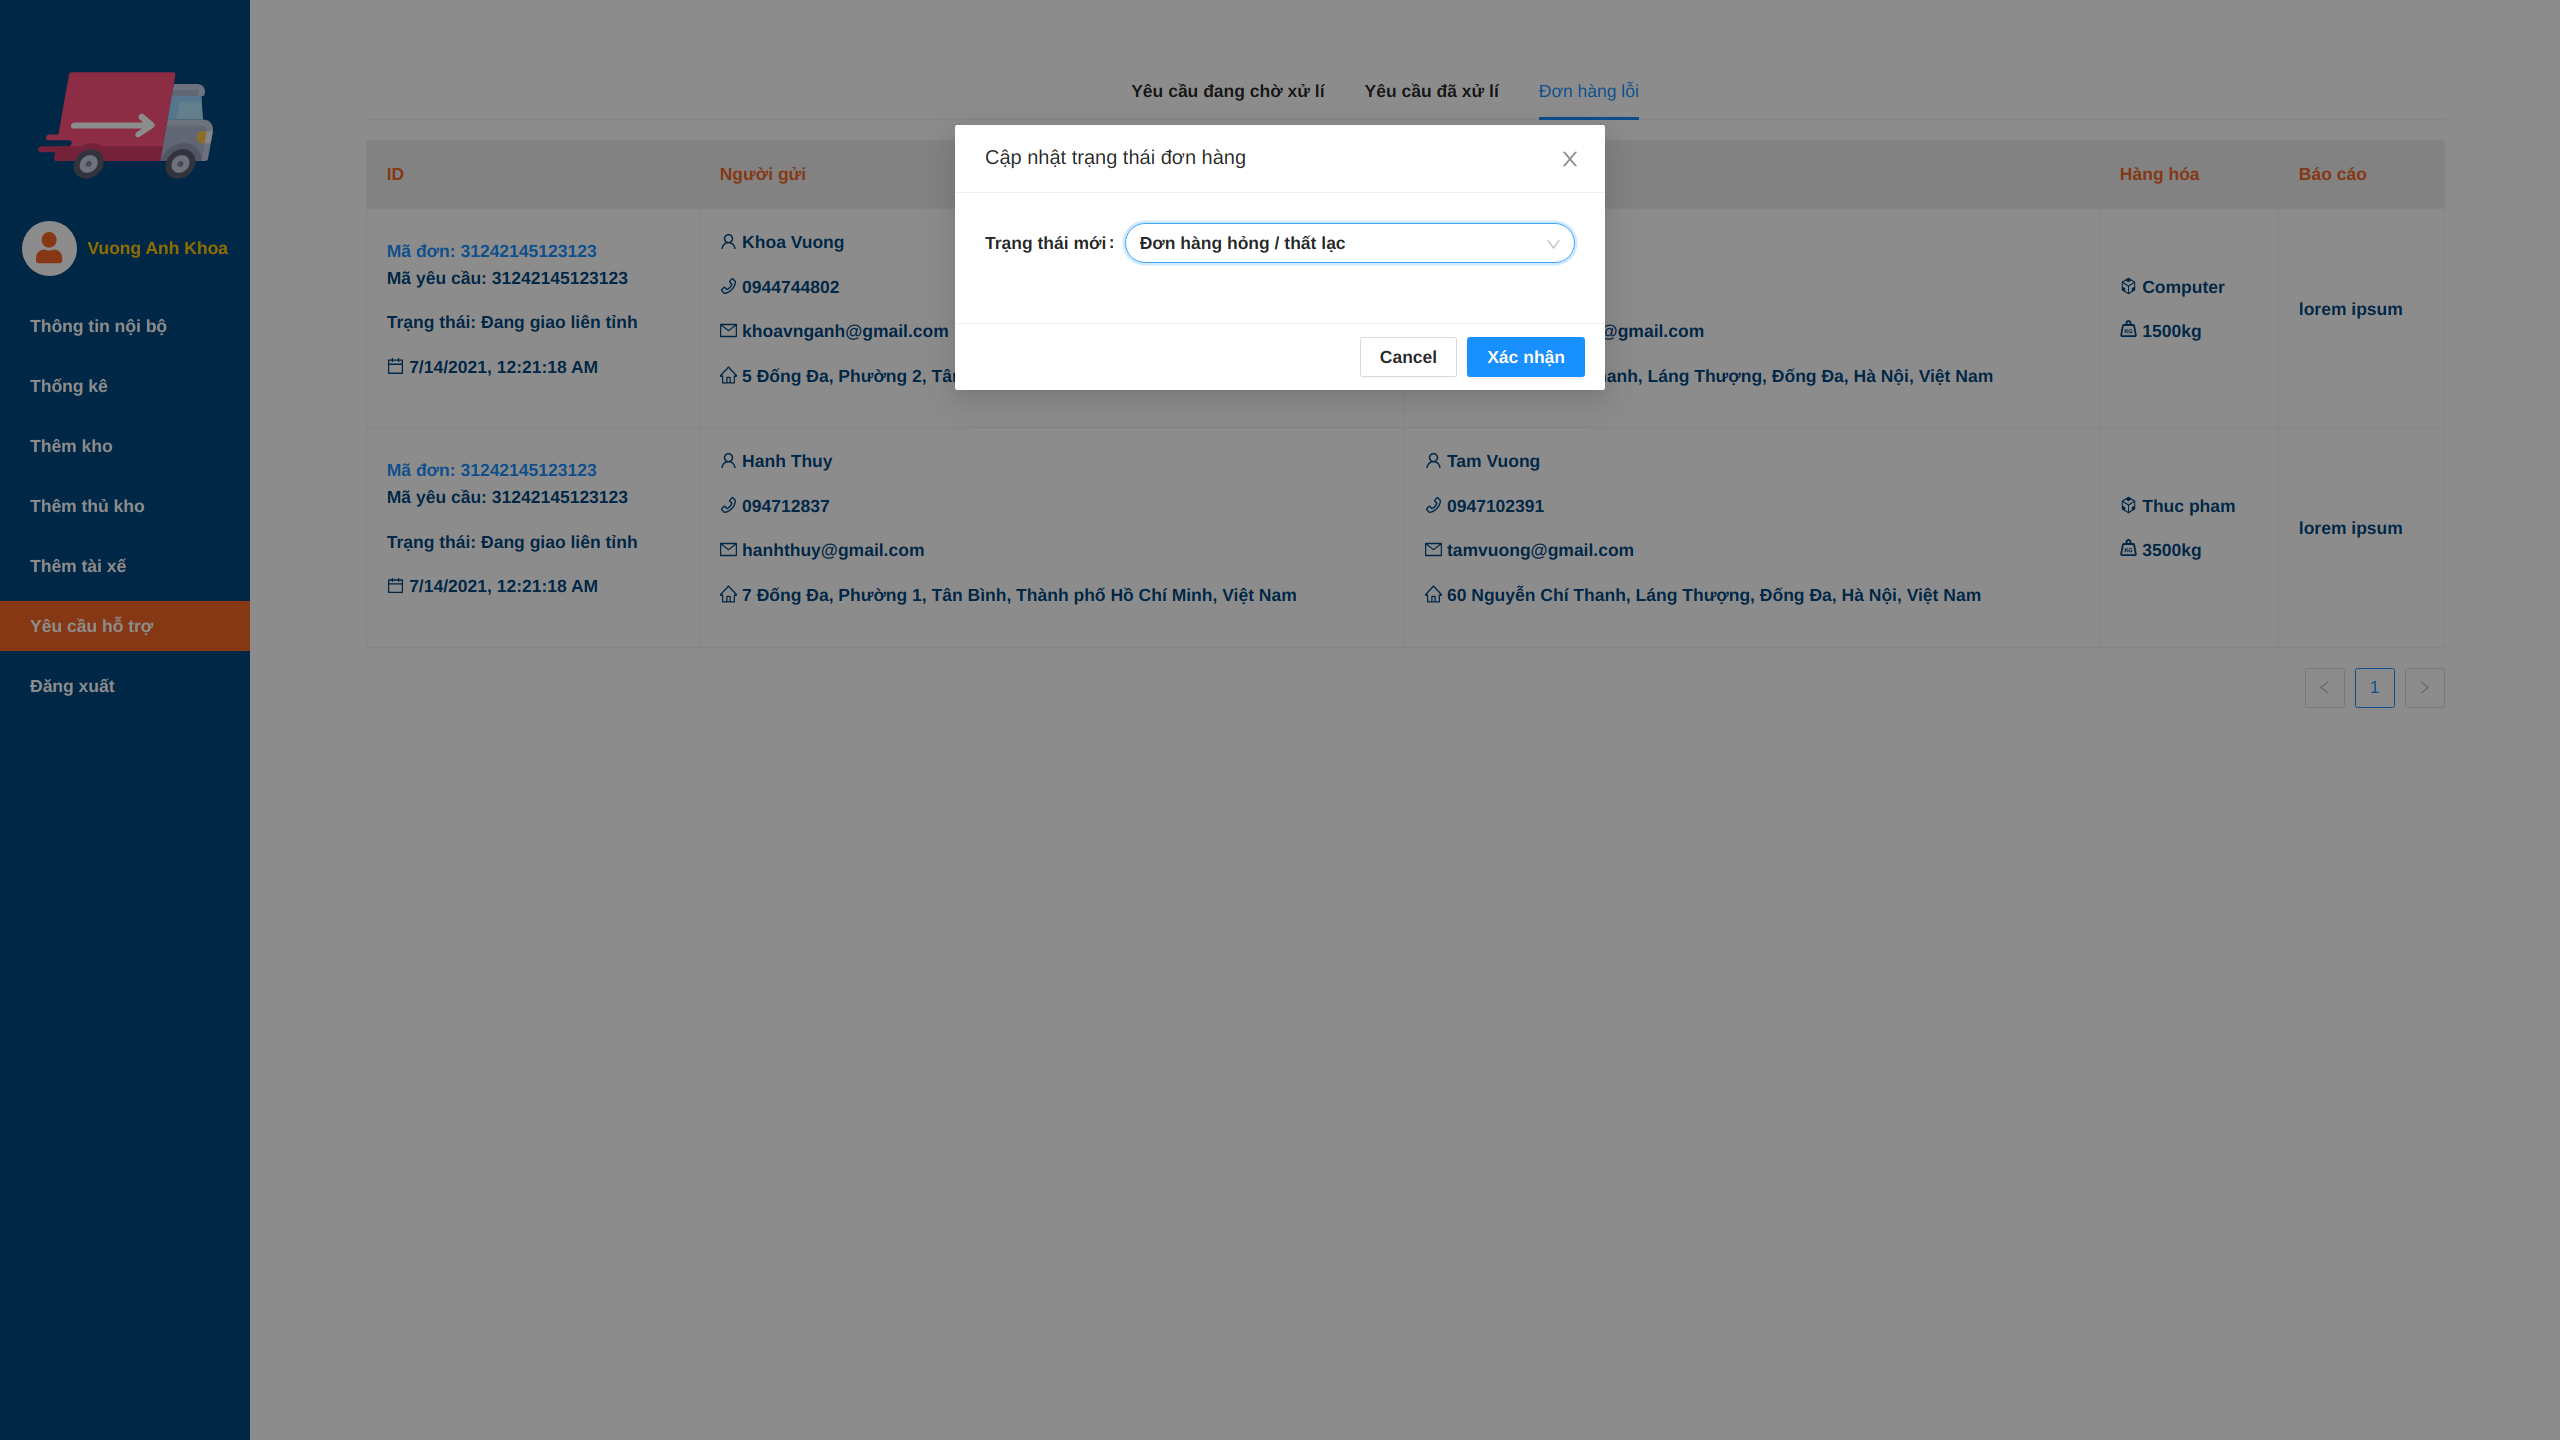
\includegraphics[width=1\textwidth]{/admin/admin_issues_reply.png}
		\centering
		\caption{Giao diện gán lại trạng thái cho những đơn có sự cố}
	\end{figure}
		
\end{itemize}

\subsection{Chức năng dành cho người nhận}
\begin{itemize}
	\item Màn hình đăng nhập của người nhận, người nhận có thể nhập mã yêu cầu để xem tình trạng của yêu cầu đó hoặc đăng nhập bằng số điện thoại để thấy tất cả các đơn hàng gửi cho mình.
	\begin{figure}[H]
		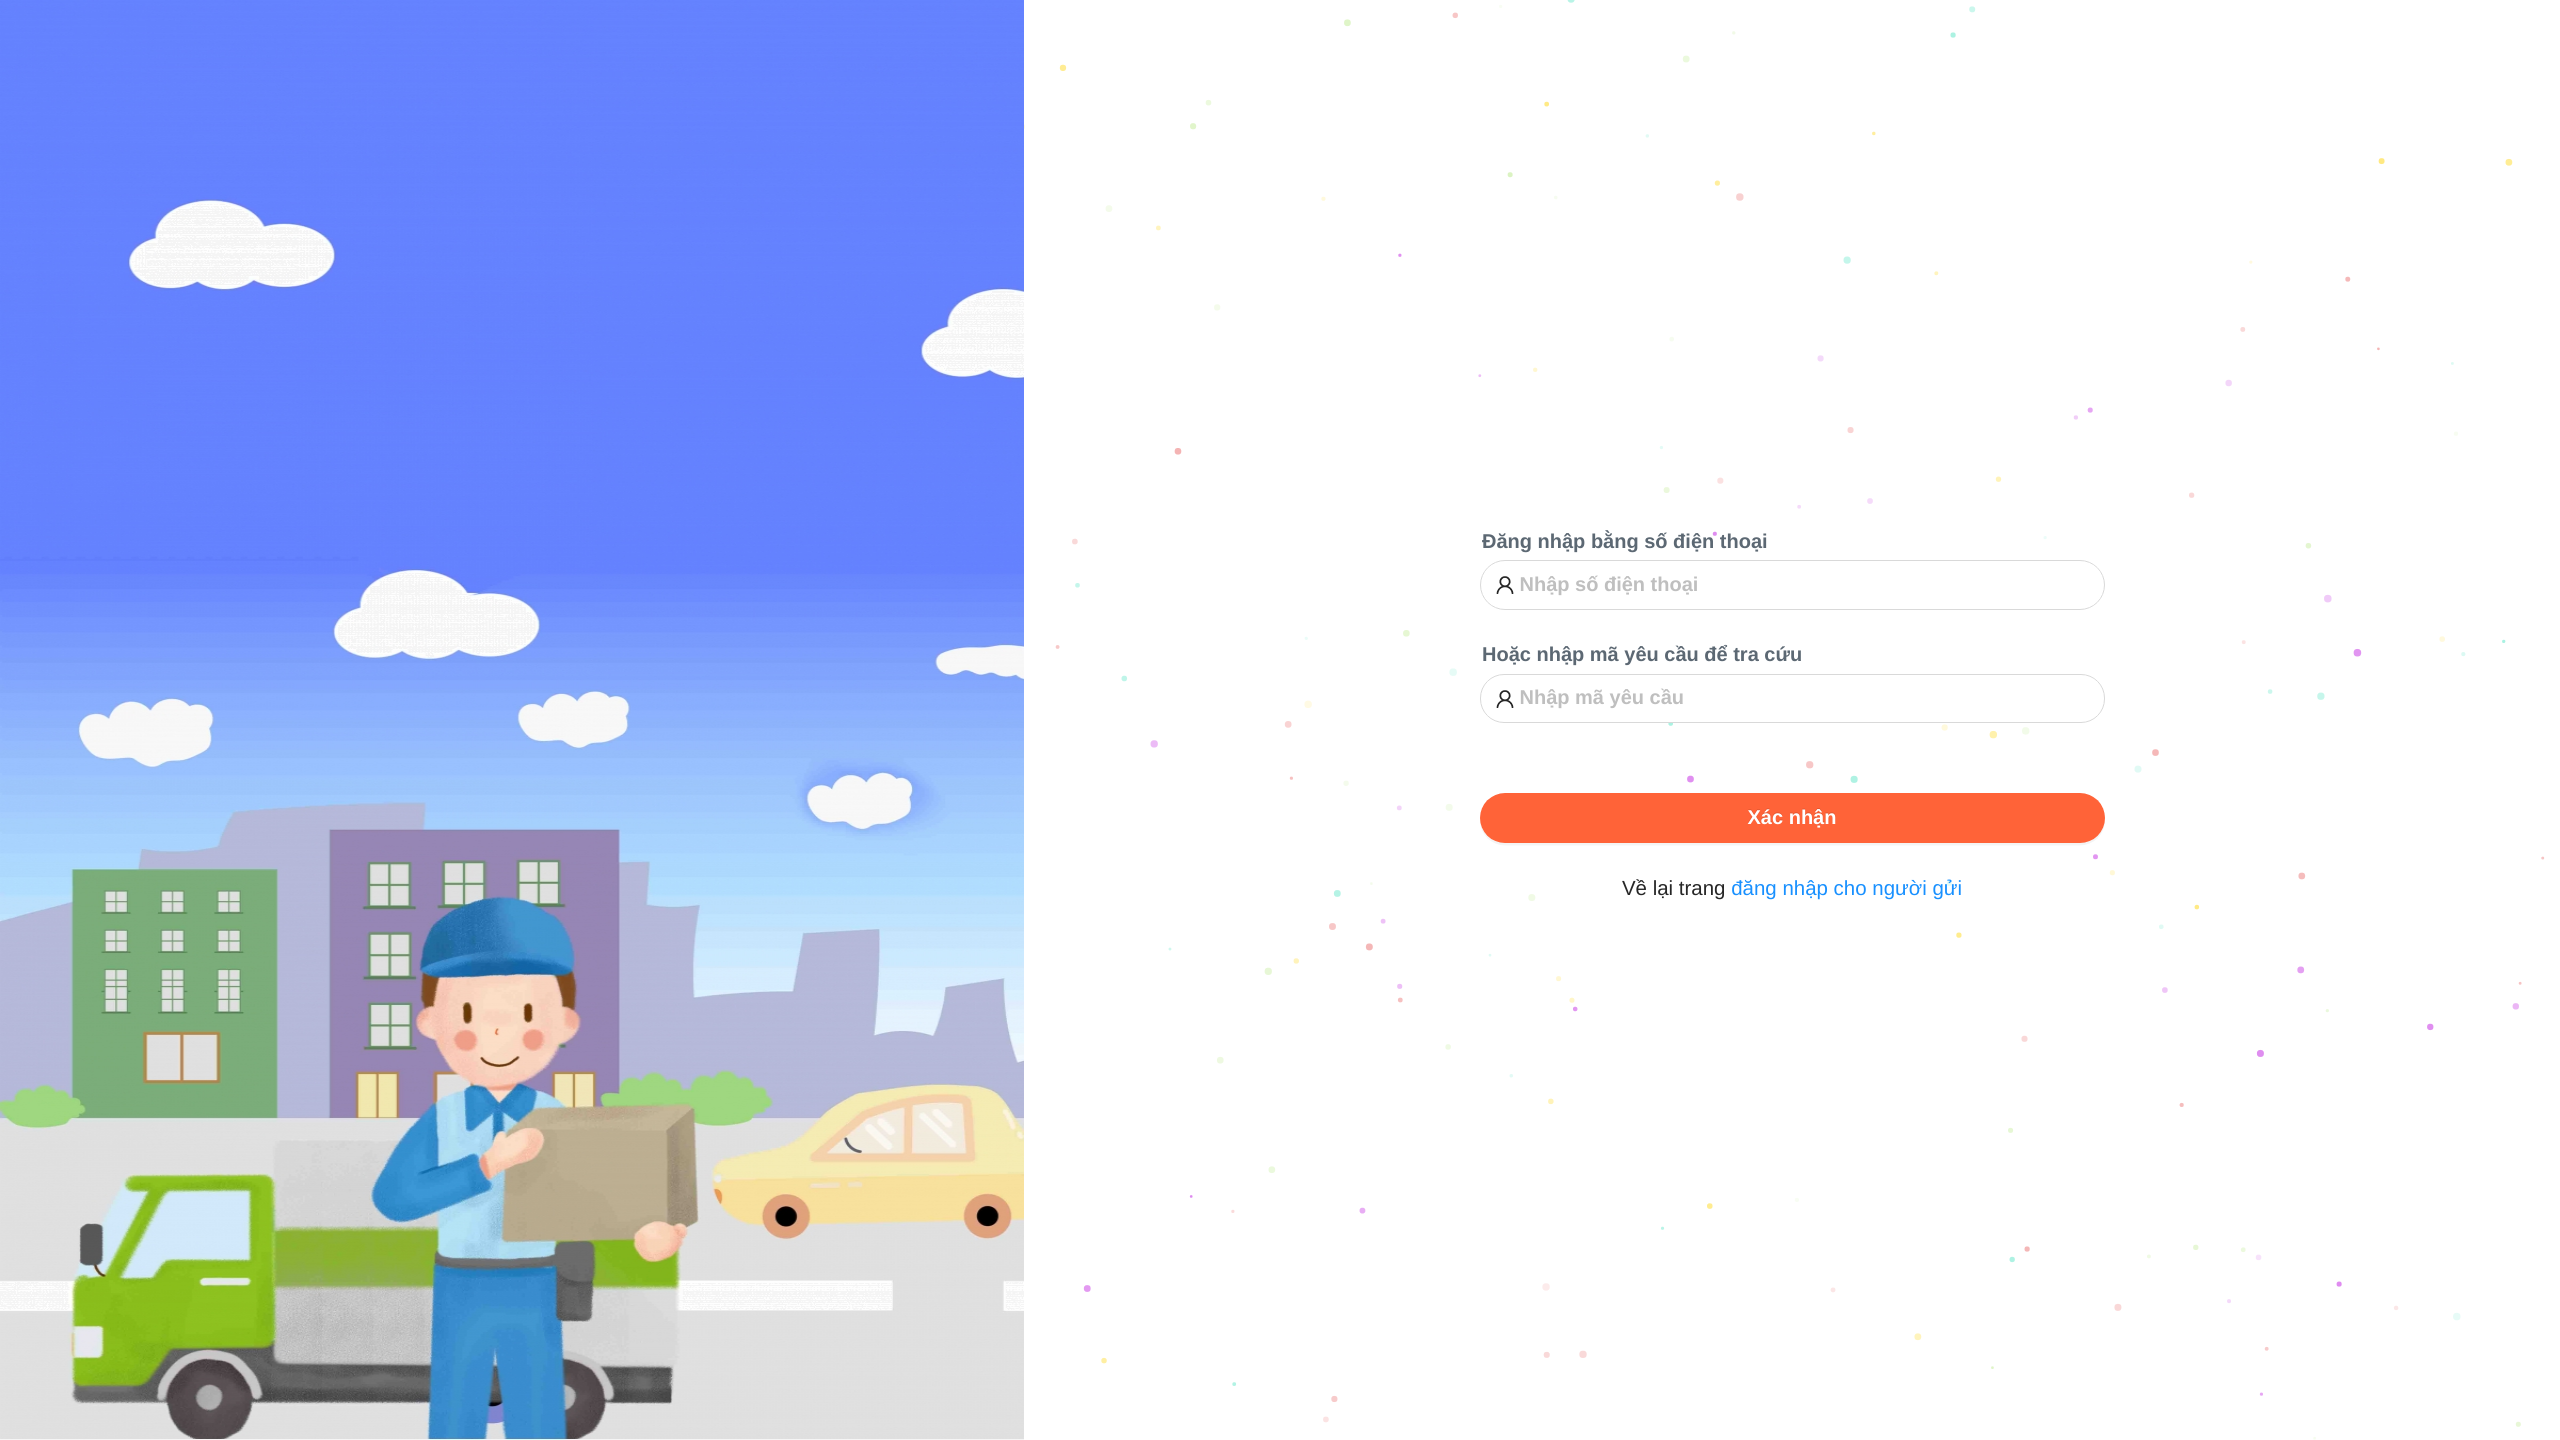
\includegraphics[width=1\textwidth]{/receiver/receiver_signin.png}
		\centering
		\caption{Giao diện đăng nhập cho người nhận}
	\end{figure}

	\item Nhập mã yêu cầu để xem thông tin và trạng thái yêu cầu và các đơn hàng liên quan.
	\begin{figure}[H]
		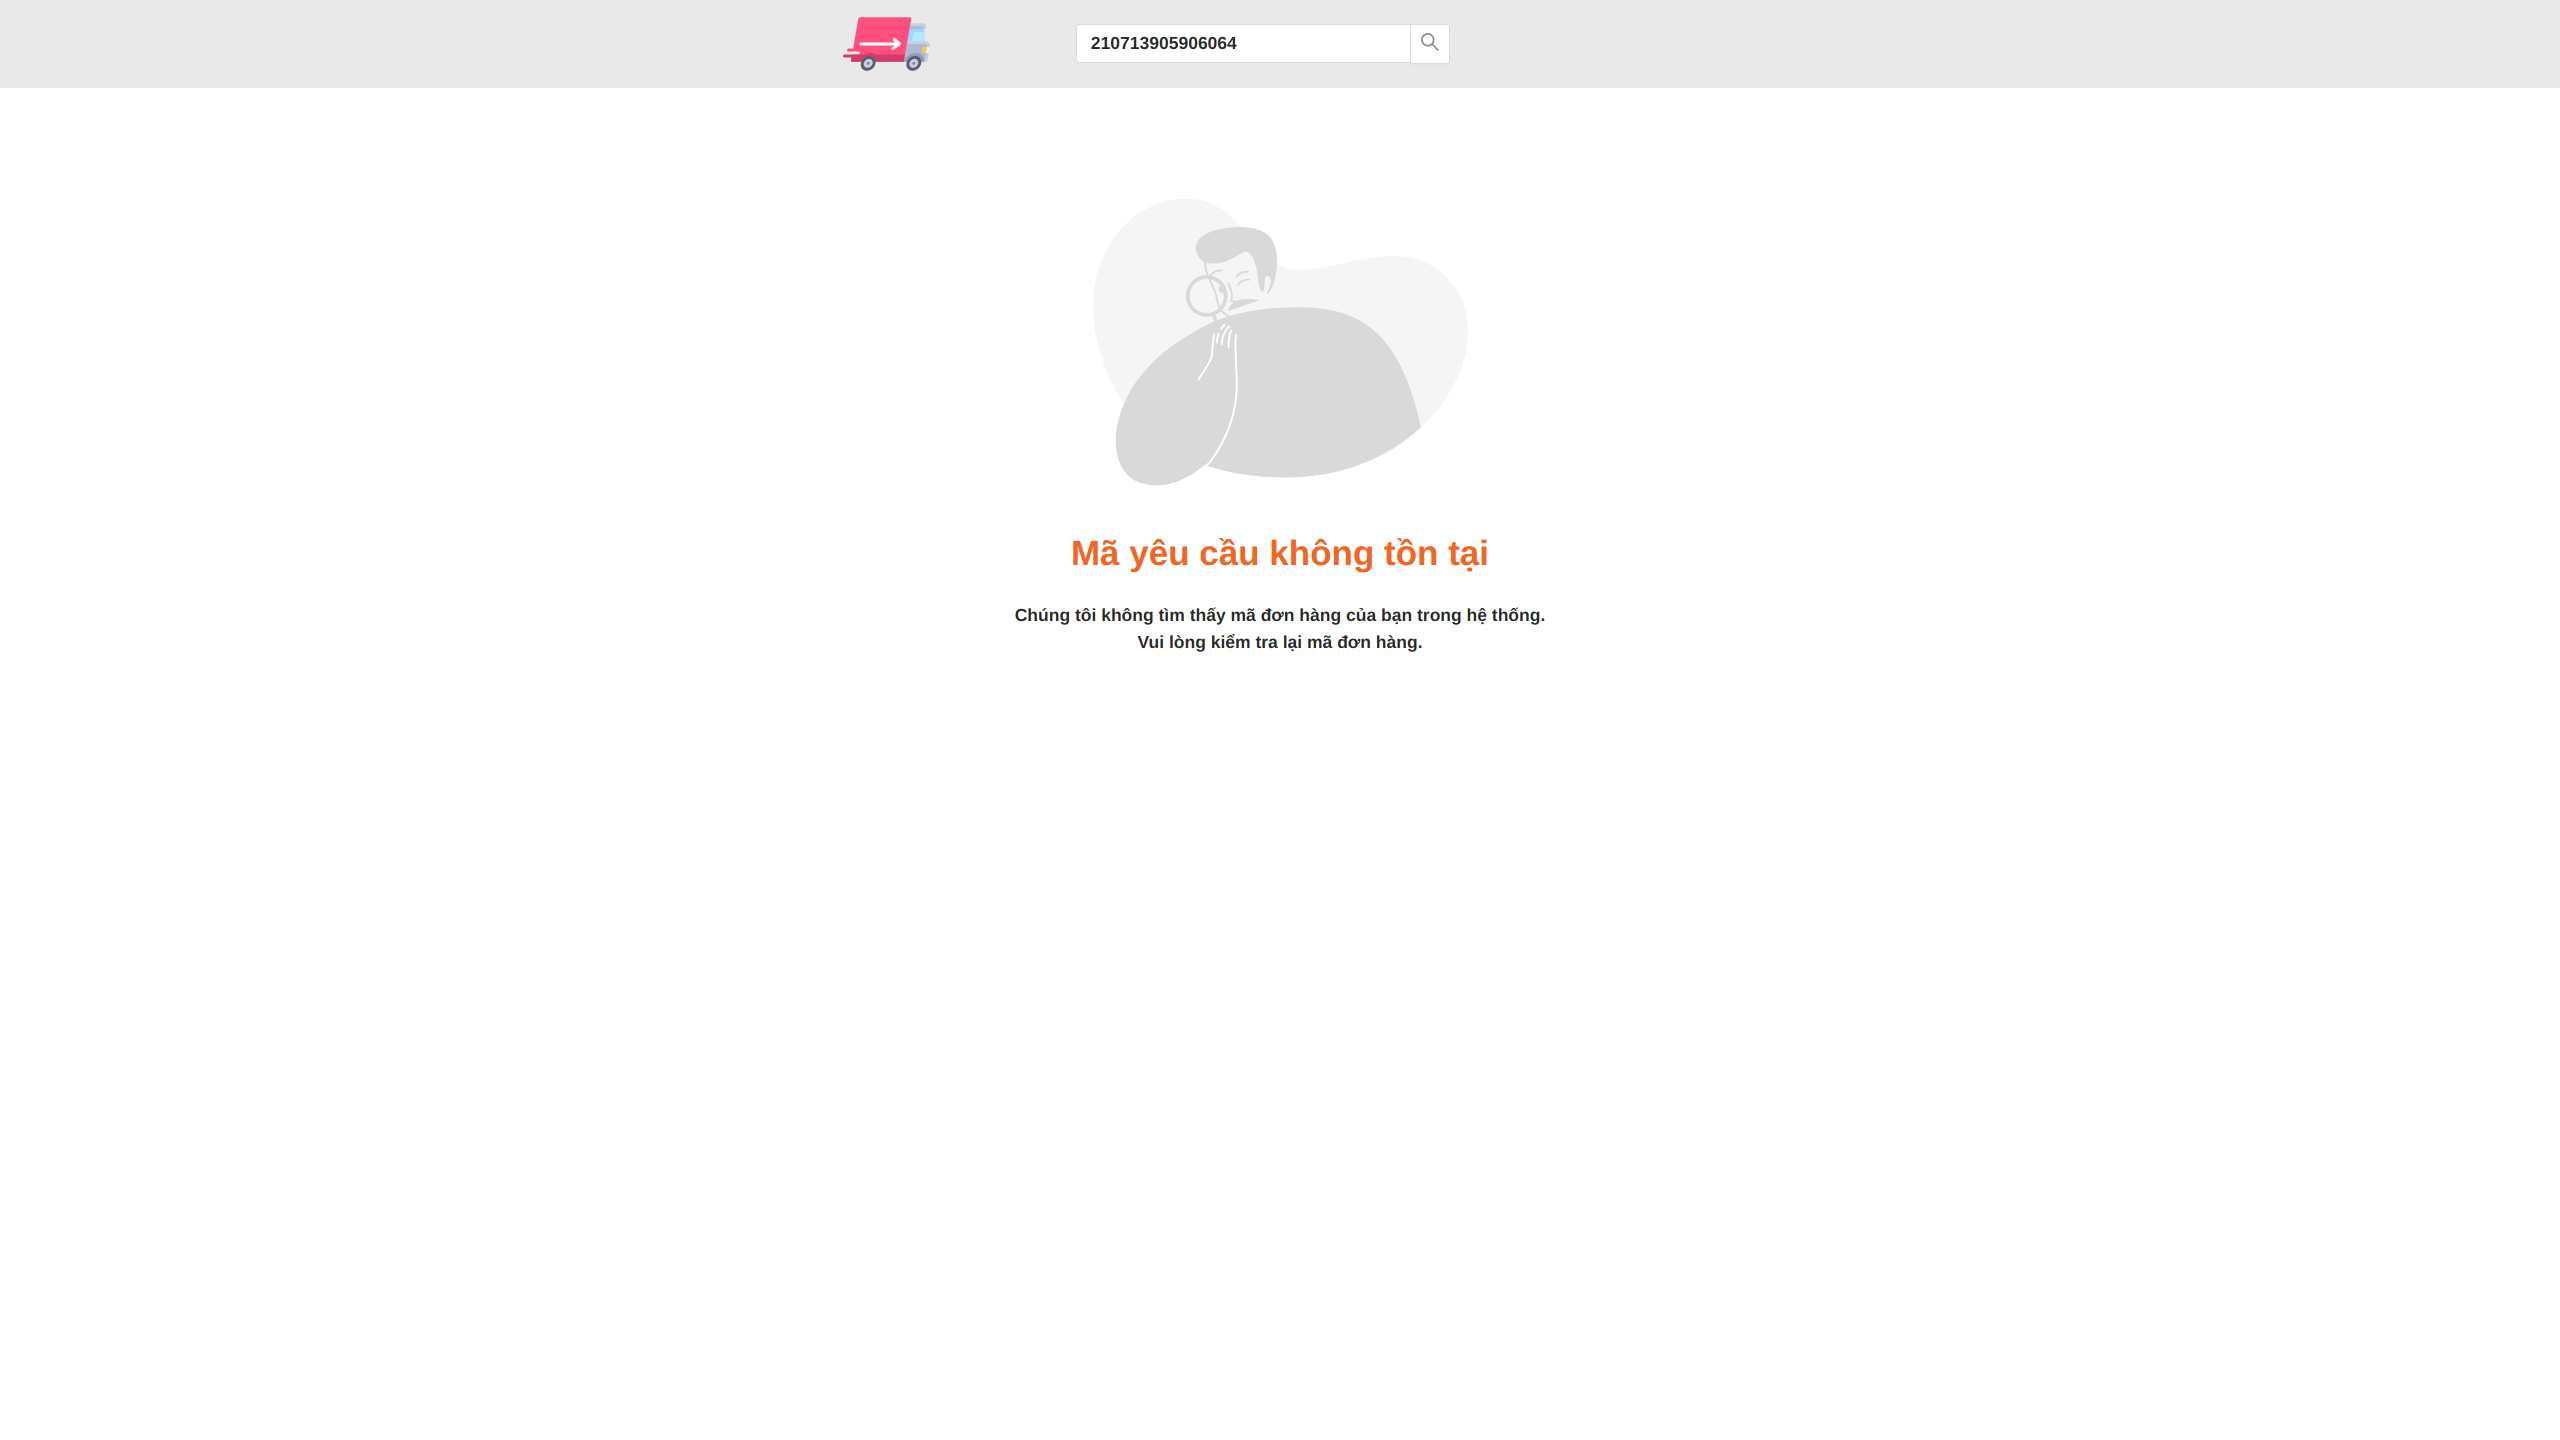
\includegraphics[width=1\textwidth]{/receiver/receiver_order_not_found.png}
		\centering
		\caption{Giao diện không tìm thẫy mã yêu cầu}
	\end{figure}

	\begin{figure}[H]
		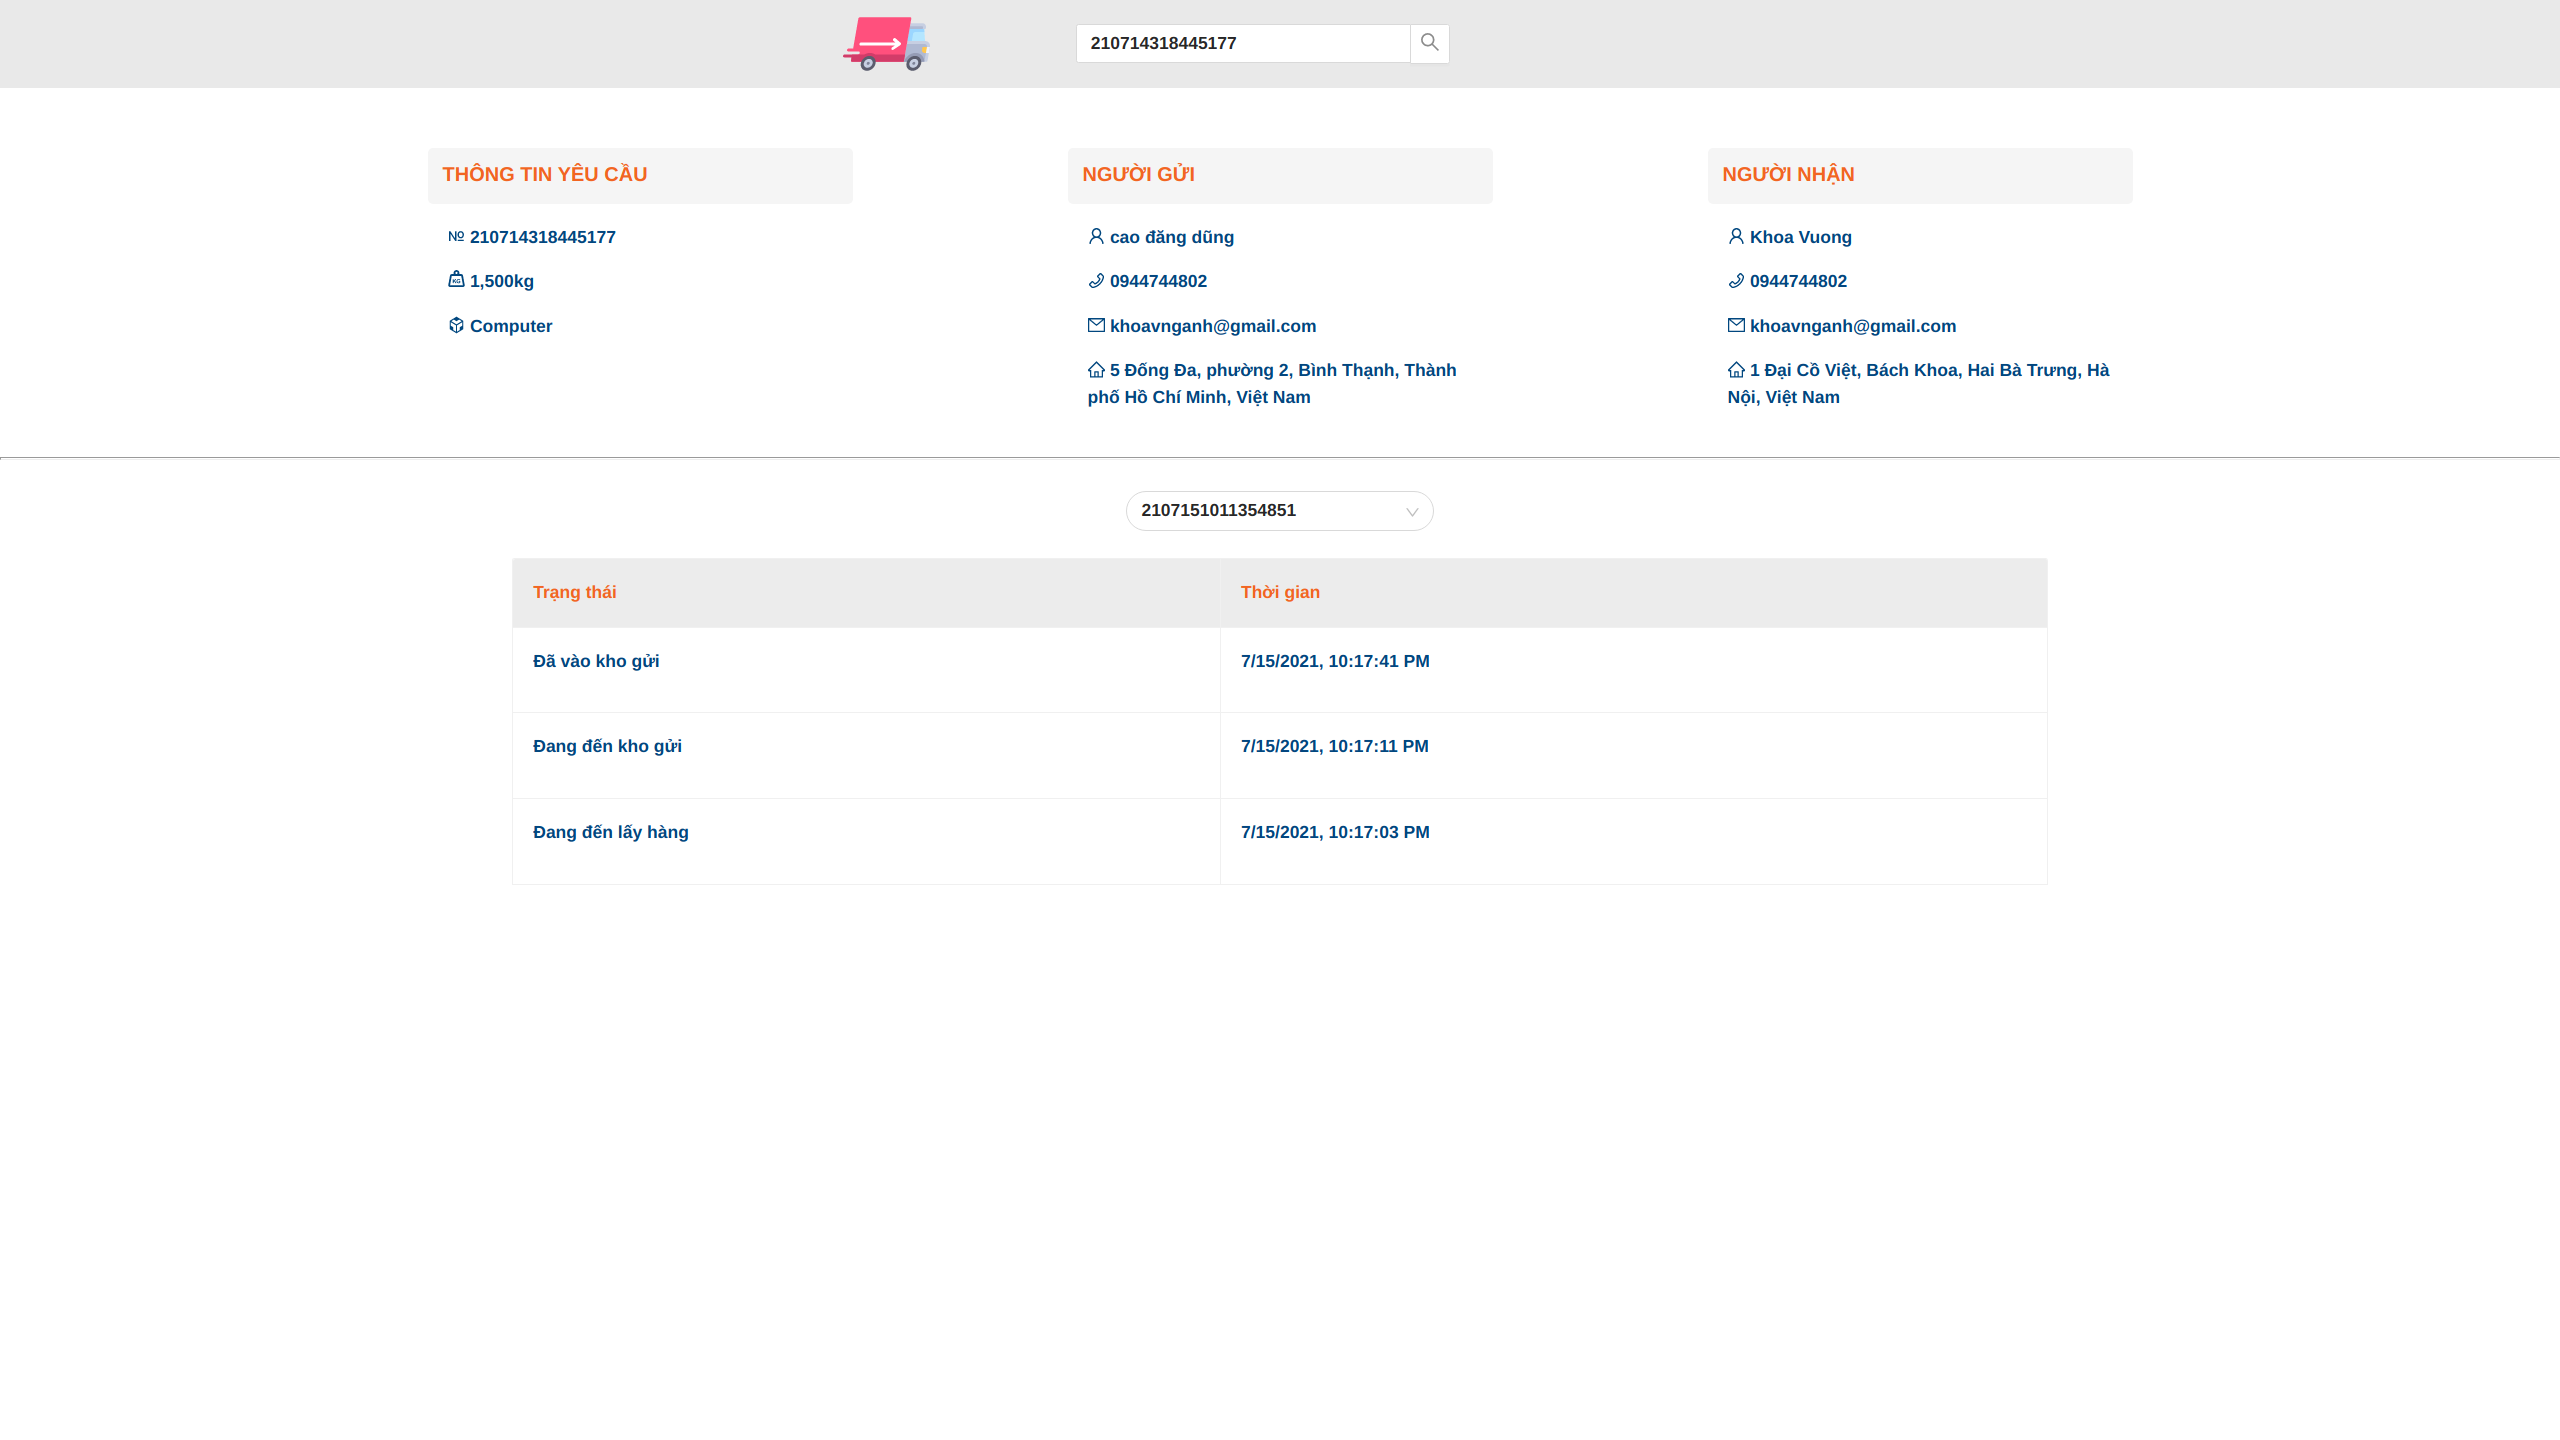
\includegraphics[width=1\textwidth]{/receiver/receiver_order_found.png}
		\centering
		\caption{Giao diện tìm thẫy mã yêu cầu}
	\end{figure}

	\item Nhập số điện thoại và mã OTP.
	\begin{figure}[H]
		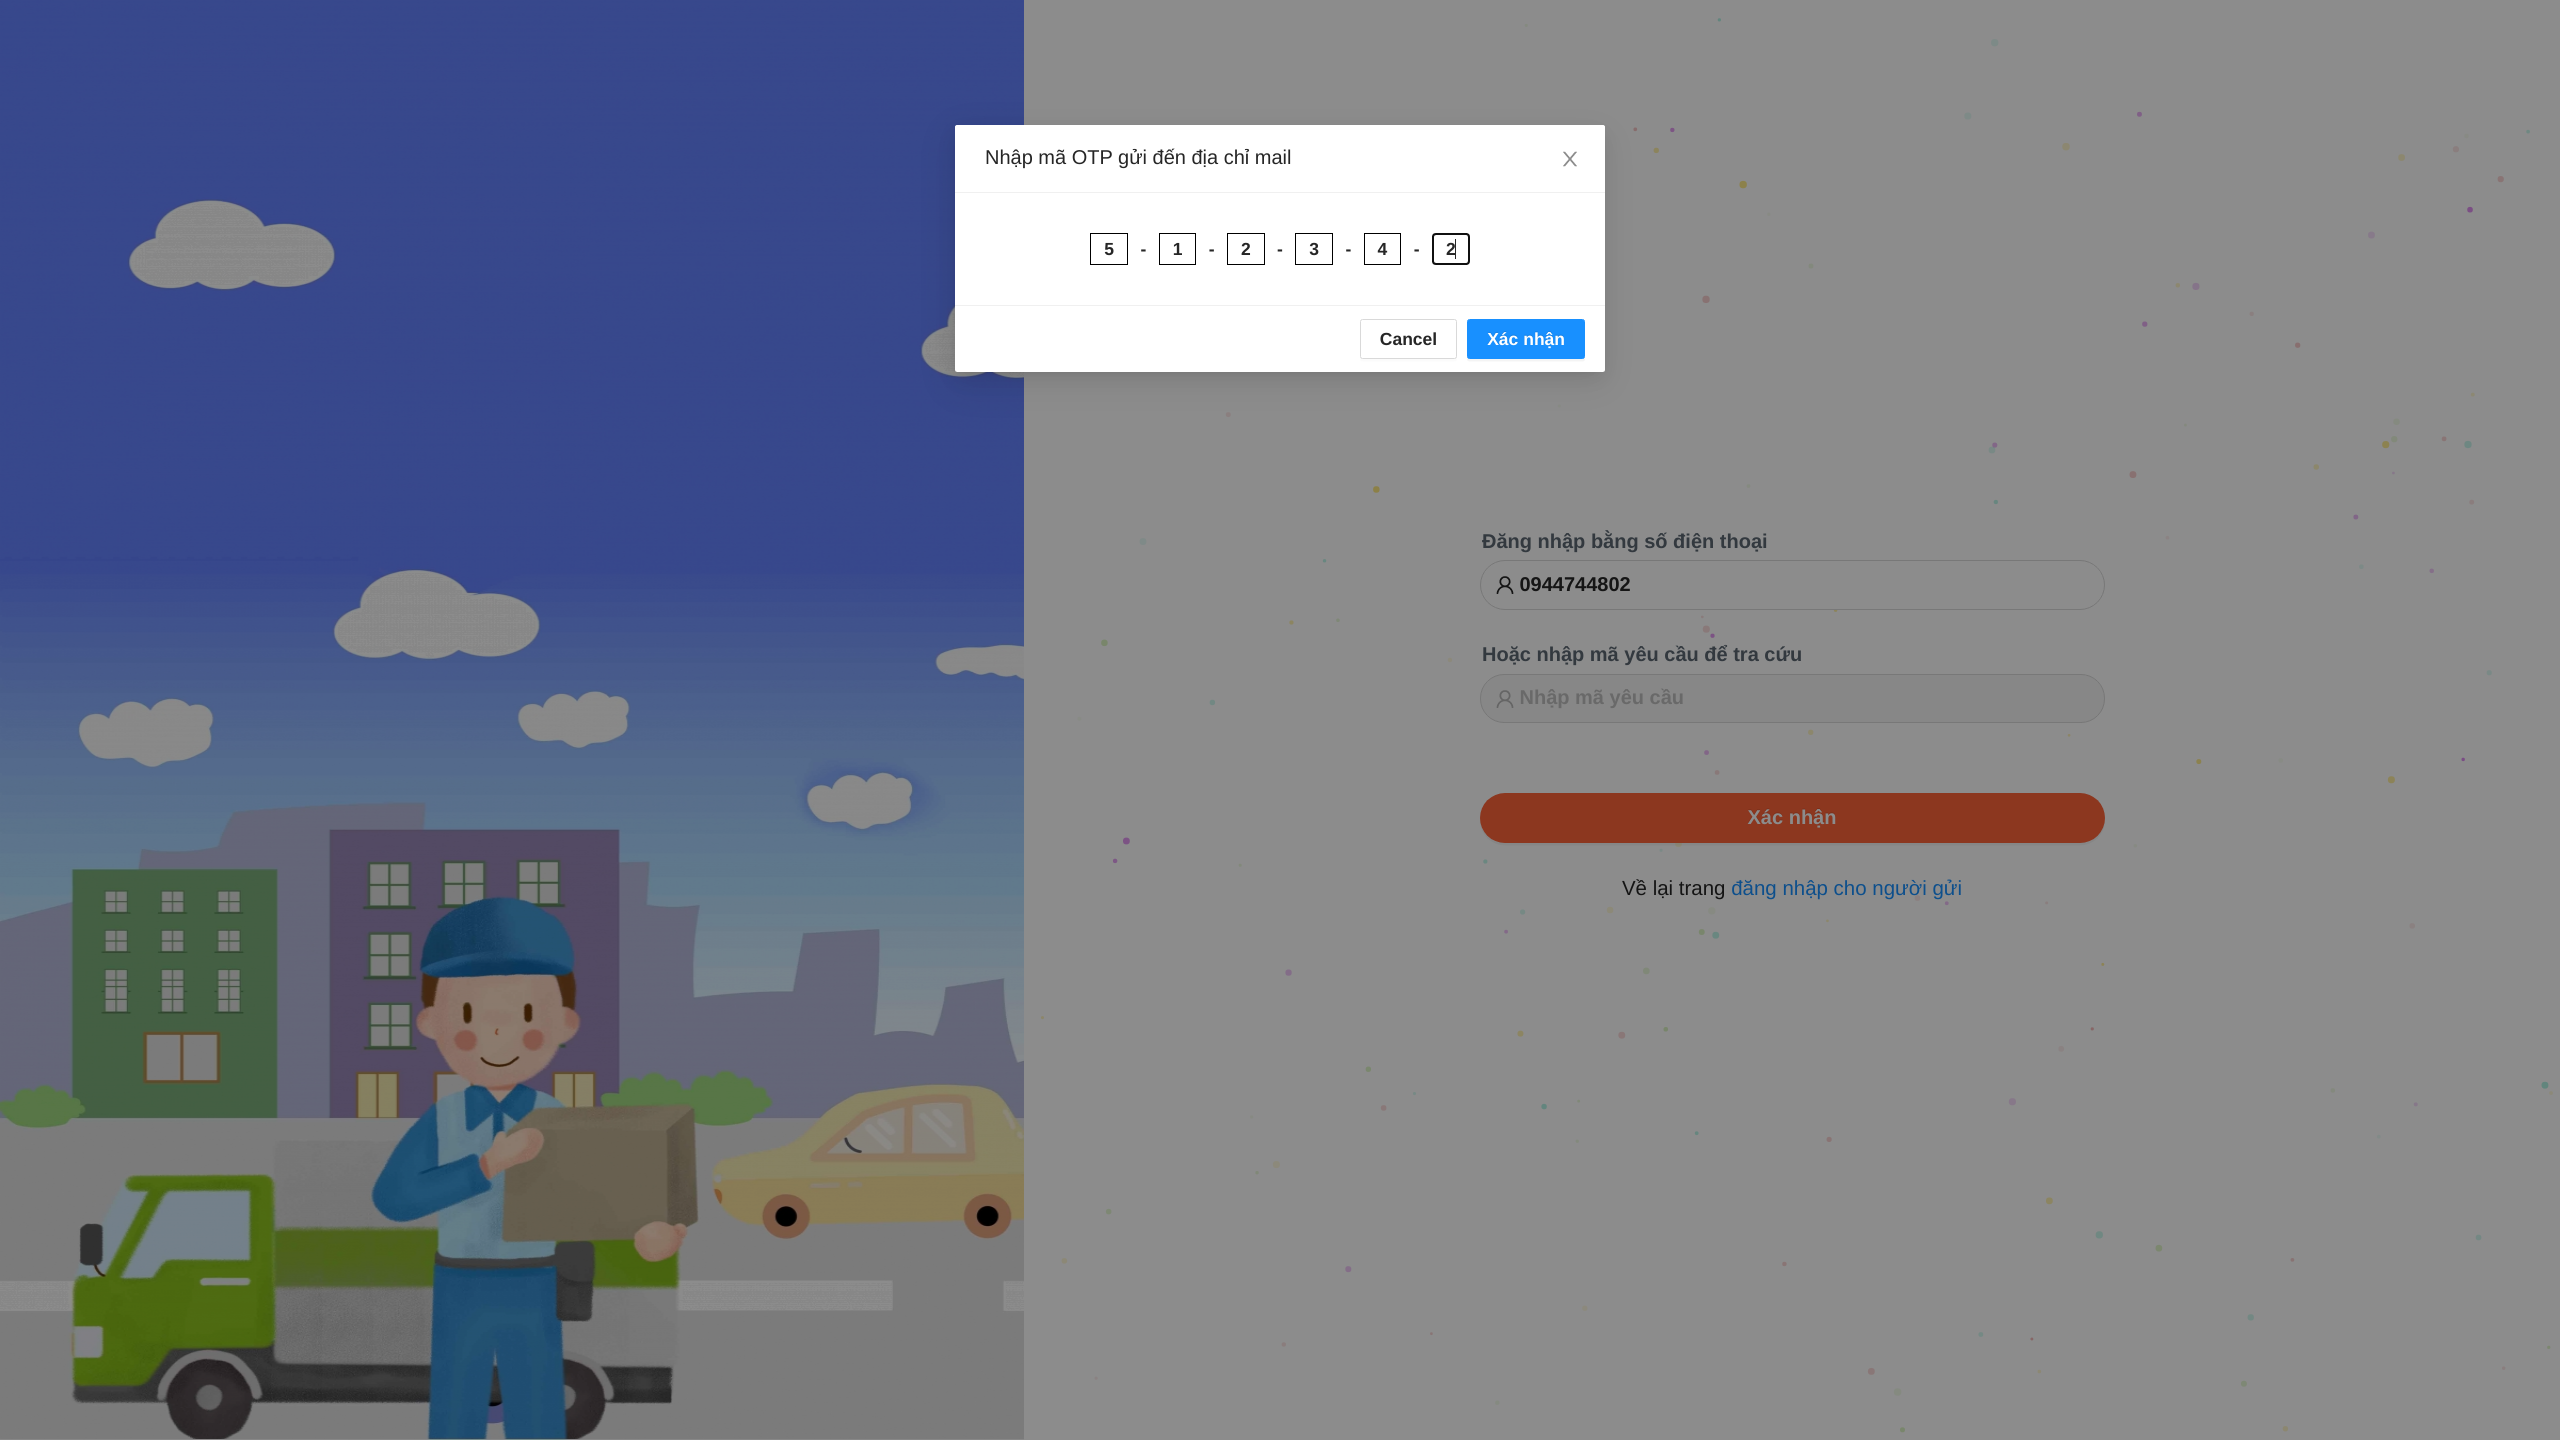
\includegraphics[width=1\textwidth]{/receiver/receiver_otp.png}
		\centering
		\caption{Giao diện nhập mã OTP nếu chọn theo dõi yêu cầu bằng số điện thoại}
	\end{figure}

	\item Nếu nhập mã OTP thành công, người nhận sẽ được đưa đến giao diện để xem các yêu cầu và đơn hàng được gửi cho mình
	
	\begin{figure}[H]
		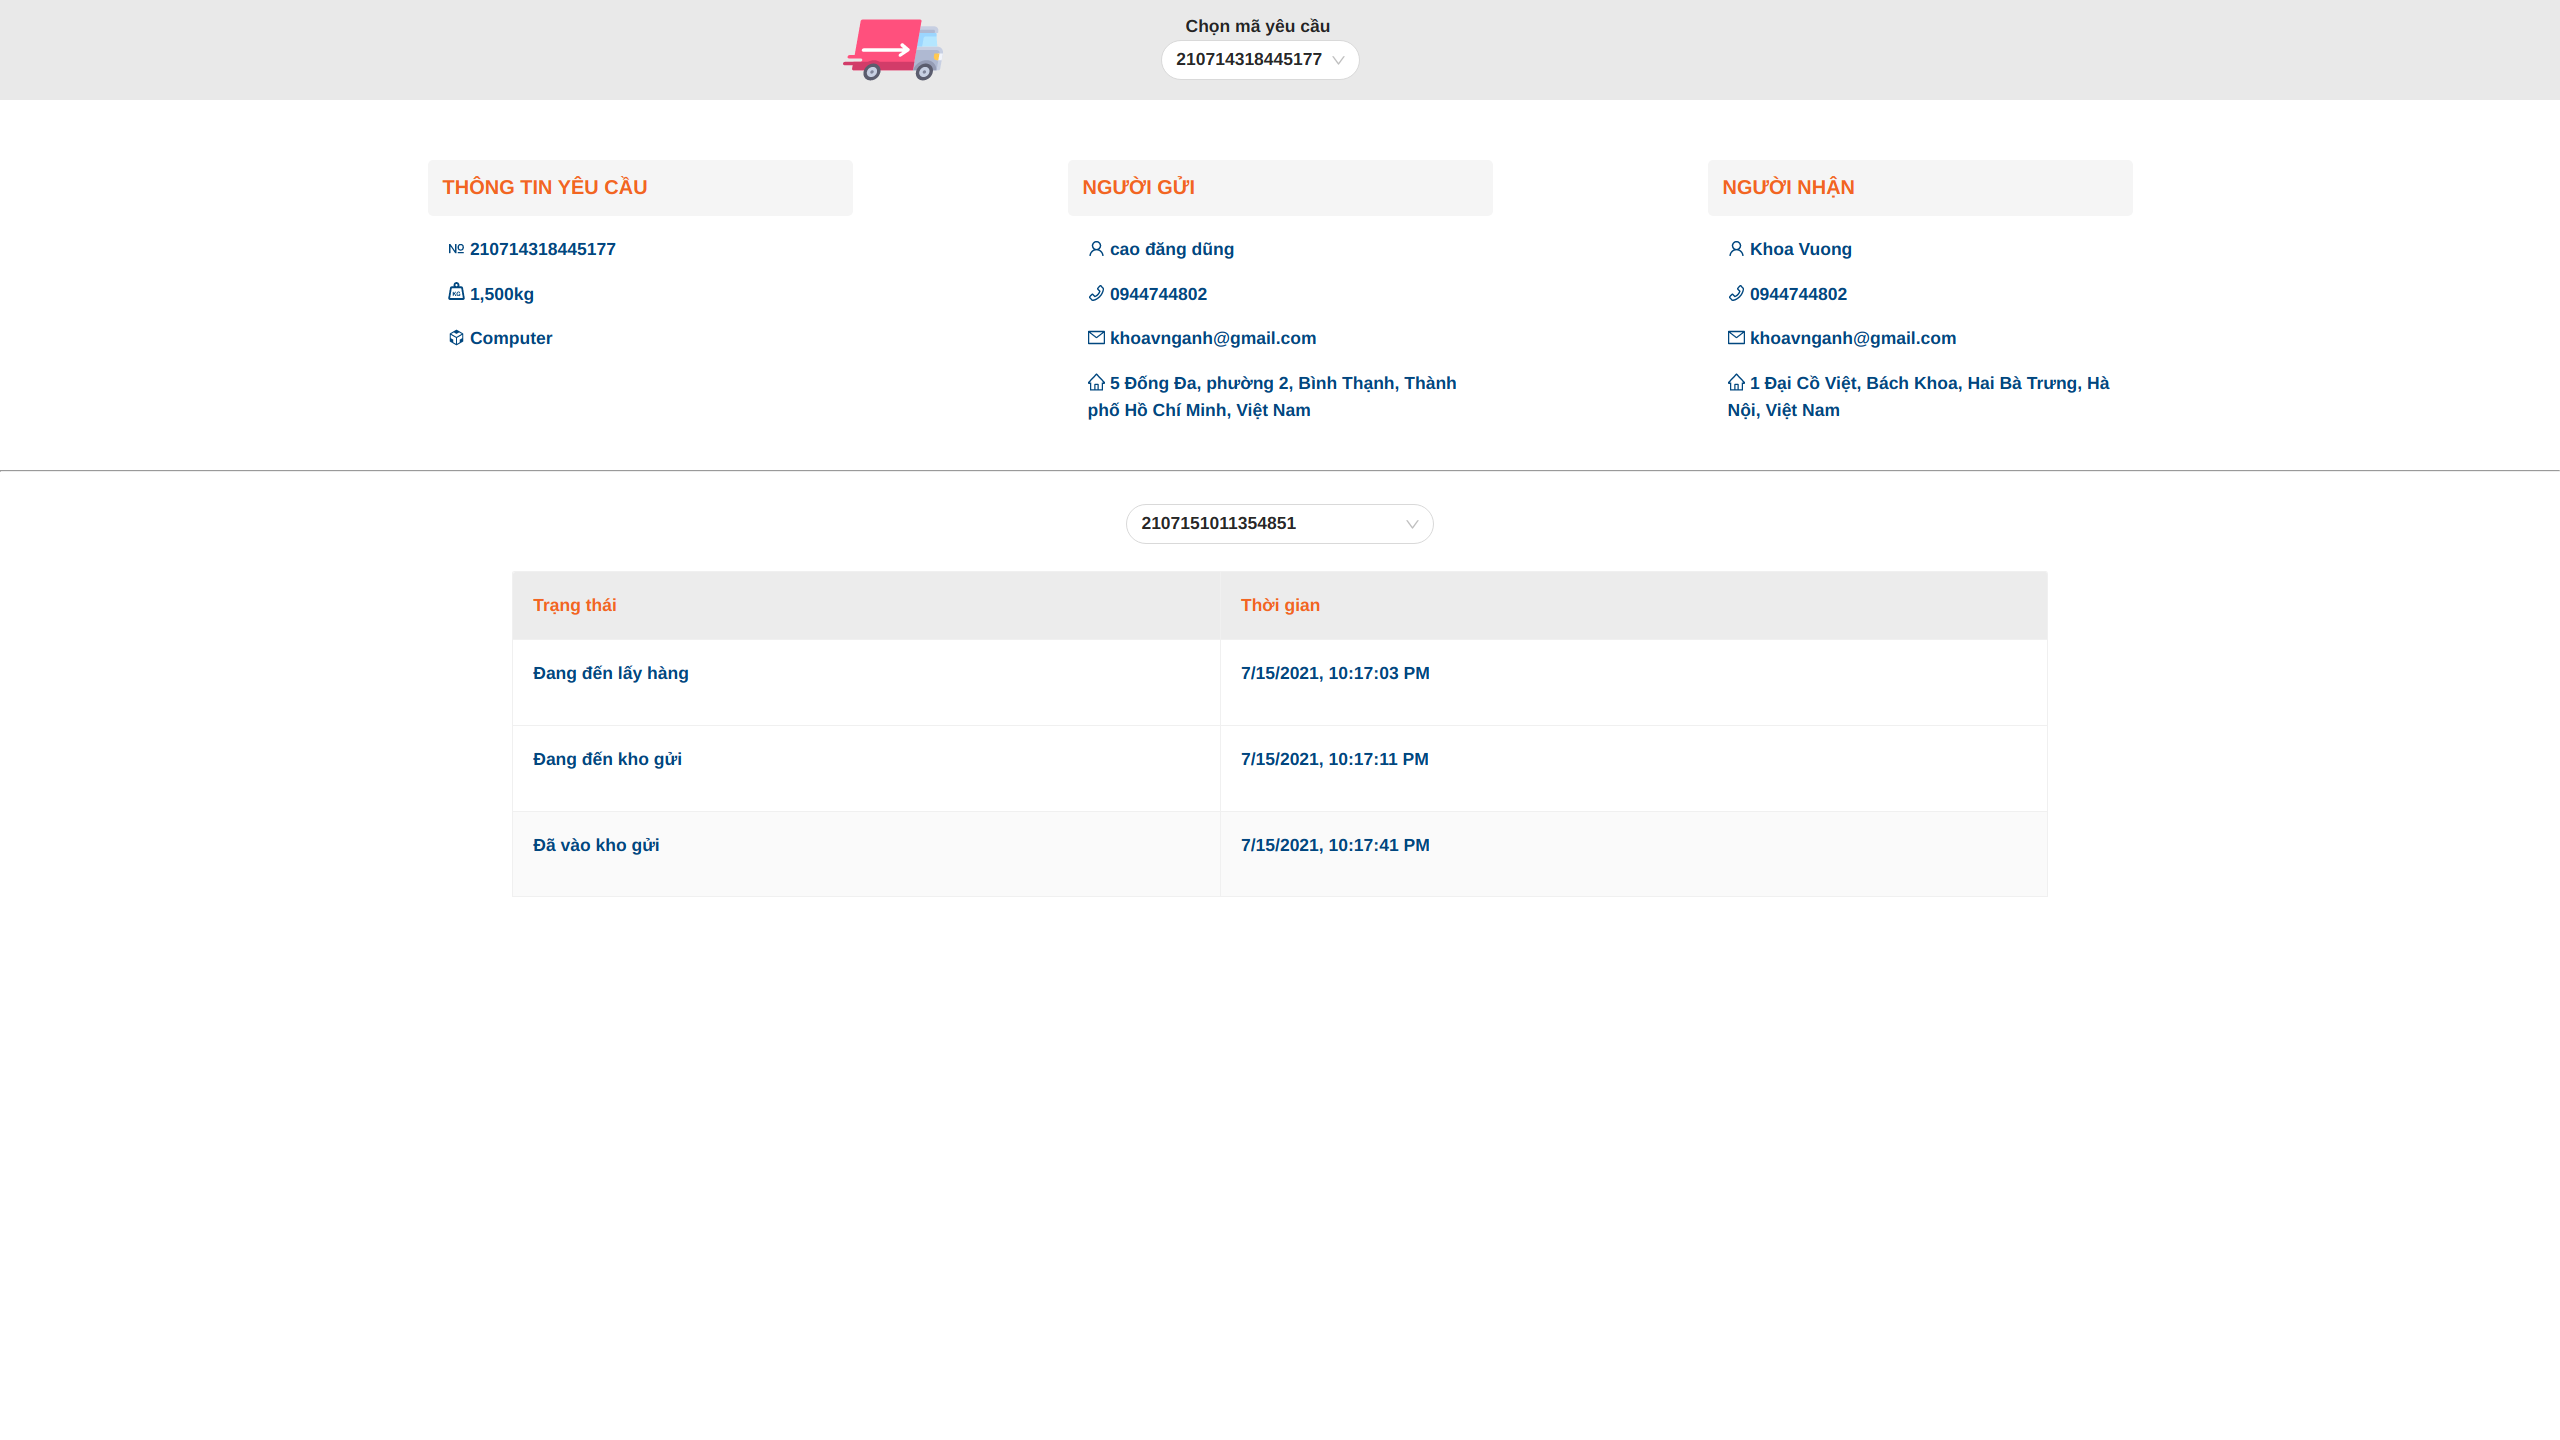
\includegraphics[width=1\textwidth]{/receiver/receiver_phone_result.png}
		\centering
		\caption{Giao diện các yêu cầu và đơn hàng của người nhận}
	\end{figure}
\end{itemize}





















